% This is the template used for the GIH thesis. It is based on 
% Reed College LaTeX thesis template. Most of the work (Reed template)
% for the document class was done by Sam Noble (SN), as well as this
% template. Later comments etc. by Ben Salzberg (BTS). Additional
% restructuring and APA support by Jess Youngberg (JY).
%
% See http://web.reed.edu/cis/help/latex.html for help. There are a
% great bunch of help pages there, with notes on
% getting started, bibtex, etc. Go there and read it if you're not
% already familiar with LaTeX.
%
% Any line that starts with a percent symbol is a comment.
% They won't show up in the document, and are useful for notes
% to yourself and explaining commands.
% Commenting also removes a line from the document;
% very handy for troubleshooting problems. -BTS

% The template was updated by Daniel Hammarström to fit GIH
% requirements. Additional code was borrowed from the 
% Stockholm University (Andreas Solders 2011) template.

% The template was forked from the thesisdown package (CII updates)

%%
%% Preamble
%%
% \documentclass{<something>} must begin each LaTeX document
\documentclass[twoside,10pt]{gihclass} %Default style using S5 paper
% Packages are extensions to the basic LaTeX functions. Whatever you
% want to typeset, there is probably a package out there for it.
% Chemistry (chemtex), screenplays, you name it.
% Check out CTAN to see: http://www.ctan.org/
%%
\usepackage{graphicx,latexsym}
\usepackage{amsmath}
\usepackage{amssymb,amsthm}
\usepackage{longtable,booktabs,setspace}
\usepackage{chemarr} %% Useful for one reaction arrow, useless if you're not a chem major
\usepackage[hyphens]{url}
% Added by CII
\usepackage{hyperref,xcolor}
\hypersetup{
    colorlinks = false,
    pdfborder={0 0 0}
}
\usepackage{lmodern}
\usepackage{float}
\floatplacement{figure}{H}
% End of CII addition
\usepackage{rotating}

% Next line commented out by CII
%%% \usepackage{natbib}
% Comment out the natbib line above and uncomment the following two lines to use the new
% biblatex-chicago style, for Chicago A. Also make some changes at the end where the
% bibliography is included.
%\usepackage{biblatex-chicago}
%\bibliography{thesis}


% Added by CII (Thanks, Hadley!)
% Use ref for internal links
\renewcommand{\hyperref}[2][???]{\autoref{#1}}
\def\chapterautorefname{Chapter}
\def\sectionautorefname{Section}
\def\subsectionautorefname{Subsection}
% End of CII addition

% Added by CII
\usepackage{caption}
\captionsetup{width=5in}
% End of CII addition


% \usepackage{times} % other fonts are available like times, bookman, charter, palatino


% Syntax highlighting #22

% To pass between YAML and LaTeX the dollar signs are added by CII

% New variables 2019-02-06 GIH copyright info 
\isbn{Provided by the library} 
\place{Stockholm}
\printeby{Printer service, Stockholm, 2019}
\coverinfo{}
\year{2019}



\title{Determinants of intra-individual variation in adaptability to resistance training of different volumes with special reference to skeletal muscle phenotypes}
\author{Daniel Hammarström}
% The month and year that you submit your FINAL draft TO THE LIBRARY (May or December)
\date{May 20xx}


%If you have two advisors for some reason, you can use the following
% Uncommented out by CII
\sernr{999}
% End of CII addition
%%% Remember to use the correct department!

% if you're writing a thesis in an interdisciplinary major,
% uncomment the line below and change the text as appropriate.
% check the Senior Handbook if unsure.
%\thedivisionof{The Established Interdisciplinary Committee for}
% if you want the approval page to say "Approved for the Committee",
% uncomment the next line
%\approvedforthe{Committee}

% Added by CII
%%% Copied from knitr
%% maxwidth is the original width if it's less than linewidth
%% otherwise use linewidth (to make sure the graphics do not exceed the margin)
\makeatletter
\def\maxwidth{ %
  \ifdim\Gin@nat@width>\linewidth
    \linewidth
  \else
    \Gin@nat@width
  \fi
}
\makeatother

\renewcommand{\contentsname}{Table of Contents}
% End of CII addition

\setlength{\parskip}{0pt}

% Added by CII

\providecommand{\tightlist}{%
  \setlength{\itemsep}{0pt}\setlength{\parskip}{0pt}}




\Dedication{
You can have a dedication here if you wish.
}

\Preface{

}

\Abstract{
The preface pretty much says it all.

\par

Second paragraph of abstract starts here.
}

\Listofpapers{
\begin{enumerate}
\def\labelenumi{\Roman{enumi}.}
\item
  \textbf{Hammarström D}, Øfsteng S, Koll L, Hanestadhaugen M, Hollan I, Apró W, Blomstrand E, Rønnestad B, Ellefsen S Benefits of higher resistance-training volume are related to ribosome biogenesis. The \emph{Journal of physiology}. 2020 Feb;598(3):543-565. doi: 10.1113/JP278455.
\item
  Khan Y, \textbf{Hammarström D}, Rønnestad B, Ellefsen S, Ahmad R Increased biological relevance of transcriptome analyses in human skeletal muscle using a model-specific pipeline. \emph{BMC Bioinformatics}. 2020 Nov 30;21(1):548. doi: 10.1186/s12859-020-03866-y
\item
  \textbf{Hammarström D}, Øfsteng S, Jacobsen N, Flobergseter K, Rønnestad B, Ellefsen S Ribosome accumulation during early phase resistance training. \emph{Manuscript}
\end{enumerate}
}


	\usepackage{lettrine} \usepackage{booktabs} \usepackage{longtable} \usepackage{array} \usepackage{multirow} \usepackage{wrapfig} \usepackage{float} \usepackage{colortbl} \usepackage{pdflscape} \usepackage{tabu} \usepackage{threeparttable} \usepackage{threeparttablex} \usepackage[normalem]{ulem} \usepackage{makecell} \usepackage{siunitx}
	\usepackage{booktabs}
 \usepackage{longtable}
 \usepackage{array}
 \usepackage{multirow}
 \usepackage{wrapfig}
 \usepackage{float}
 \usepackage{colortbl}
 \usepackage{pdflscape}
 \usepackage{tabu}
 \usepackage{threeparttable}
 \usepackage{threeparttablex}
 \usepackage[normalem]{ulem}
 \usepackage{makecell}
% End of CII addition
%%
%% End Preamble
%%
%


% Added updated related to csl update in Pandoc
\newlength{\cslhangindent}
\setlength{\cslhangindent}{1.5em}
\newlength{\csllabelwidth}
\setlength{\csllabelwidth}{3em}
\newenvironment{CSLReferences}[3] % #1 hanging-ident, #2 entry spacing
 {% don't indent paragraphs
  \setlength{\parindent}{0pt}
  % turn on hanging indent if param 1 is 1
  \ifodd #1 \everypar{\setlength{\hangindent}{\cslhangindent}}\ignorespaces\fi
  % set entry spacing
  \ifnum #2 > 0
  \setlength{\parskip}{#2\baselineskip}
  \fi
 }%
 {}
\usepackage{calc} % for \widthof, \maxof
\newcommand{\CSLBlock}[1]{#1\hfill\break}
\newcommand{\CSLLeftMargin}[1]{\parbox[t]{\maxof{\widthof{#1}}{\csllabelwidth}}{#1}}
\newcommand{\CSLRightInline}[1]{\parbox[t]{\linewidth}{#1}}
\newcommand{\CSLIndent}[1]{\hspace{\cslhangindent}#1}


\begin{document}




% Everything below added by CII


\frontmatter % this stuff will be roman-numbered
% \pagestyle{empty} % this removes page numbers from the frontmatter
  \maketitle
  \begin{dedication}
  \topskip0pt
\vspace*{\fill}
 You can have a dedication here if you wish.
\vspace*{\fill}
  \end{dedication}
\begin{defence}
    THESIS FOR DOCTORAL DEGREE (Ph.D.)\\
    ~\\
    ~\\
    \textbf{The title of your thesis}\\
    ~\\
    by\\
    \textbf{Your name}\\
    ~\\
    ~\\
    Thesis for Philosophy of Doctoral Degree in Sport Sciences, at The Swedish School of Sport and Health Sciences (GIH), which, according to the decision of the dean, will be publicly defended on \emph{DATE}. The thesis defense will be held at the auditorium at The Swedish School of Sport and Health Sciences (GIH), Stockholm.\\
    ~\\
    ~\\
    \textbf{Opponent}\\
    Profesor \ldots.\\
    ~\\
    \textbf{Principal supervisor}\\
    Profesor\ldots{}\\
    ~\\
    \textbf{Co-supervisor(s)}\\
    -Professor\ldots{}\\
    -Professor\ldots{}\\
    -Professor\ldots{}\\
    ~\\
    \textbf{Examination board}\\
    -Associate professor\ldots{}\\
    -Professor \ldots{}\\
    -Professor \ldots{}
  \end{defence}

  \begin{abstract}
    The preface pretty much says it all.

    \par

    Second paragraph of abstract starts here.
  \end{abstract}
  \begin{listofpapers}
    \begin{enumerate}
    \def\labelenumi{\Roman{enumi}.}
    \item
      \textbf{Hammarström D}, Øfsteng S, Koll L, Hanestadhaugen M, Hollan I, Apró W, Blomstrand E, Rønnestad B, Ellefsen S Benefits of higher resistance-training volume are related to ribosome biogenesis. The \emph{Journal of physiology}. 2020 Feb;598(3):543-565. doi: 10.1113/JP278455.
    \item
      Khan Y, \textbf{Hammarström D}, Rønnestad B, Ellefsen S, Ahmad R Increased biological relevance of transcriptome analyses in human skeletal muscle using a model-specific pipeline. \emph{BMC Bioinformatics}. 2020 Nov 30;21(1):548. doi: 10.1186/s12859-020-03866-y
    \item
      \textbf{Hammarström D}, Øfsteng S, Jacobsen N, Flobergseter K, Rønnestad B, Ellefsen S Ribosome accumulation during early phase resistance training. \emph{Manuscript}
    \end{enumerate}
  \end{listofpapers}

  \hypersetup{linkcolor=black}
  \setcounter{tocdepth}{2}
  \tableofcontents

  \listoftables

  \listoffigures




\mainmatter % here the regular arabic numbering starts
\pagestyle{fancyplain} % turns page numbering back on

\setcounter{DefaultLines}{3}

\hypertarget{introduction}{%
\chapter{Introduction}\label{introduction}}

\lettrine{S}keletal muscle health is essential for physical independence. In a lifespan perspective, measures of muscle mass and/or strength are inversely associated with mortality
{[}1, 2, 3, 4, 5, 6, 7{]}
and disability
{[}8{]}.
Besides adverse associations between of low muscle mass and strength and clinical conditions, muscle weakness also accounts for increased health care costs in patient populations
{[}9, 10{]}.
The intercept between muscle mass, muscle function and health status is interrelated with variables such as age and primary illness or injury
{[}11{]}.
This highlights that interventions designed to increase muscle mass and strength are likely to prevent adverse health outcomes across the lifespan. A higher level of muscle mass and functional capacity would counteract the effects of muscle loss due to illness, age or inactivity.

Although a large degree of the observed variations in lean mass and strength are attributed to genetic components
{[}12, 13{]},
environmental factors also contribute, leaving a window of opportunity to increase muscle mass and functional capacity. Among factors affecting muscle mass and functioning are nutrition and pharmacological agents. However, physical activity and specifically systematic resistance training of sufficient volume, intensity and frequency provides a stimulus that promote morphological and functional changes to the human neuromuscular system without adverse side-effects. Irrespective of age, resistance training generally leads to increased muscle mass and strength
{[}14, 15{]}
and is considered safe when performed in a well organized manner
{[}15, 16{]}.

Resistance training can be modulated indefinitely through combined variations of training variables such as frequency, intensity and volume
{[}17, 18{]}.
Well designed training prescriptions should incorporate information about the current state and goals of the trainee to maximize the potential outcome of the training program
{[}17, 19, 18{]}.
Training volume has received particular attention in the scientific community for many reasons. Evidence suggests that exercise volume affects selected molecular determinants of muscle hypertrophy in a dose-dependent manner
{[}20, 21, 22{]}.
Such effects are believed to facilitate long-term training effects as training programs with higher volume generally result in higher gains in muscle mass and strength with little evidence of differences between age groups or participants with different training backgrounds
{[}23, 24, 25{]}. \\
A consequence of a more extensive training program is the increased time required to complete such a program. As time constraints has been reported as a limiting factor for engaging in physical activity
{[}26{]}
some merit can be given to arguments against guidlines suggesting higher volume in resistance training prescription
{[}27, 19{]}.
From an individual perspective, training prescription that balances time-requirement with efficacy presumably increases the likelihood of participation in physical activity {[}26{]}.
From a more general perspective, increased knowledge about mechanisms governing responses to physical training could improve training prescription also for individuals and populations that experience attenuated benefit of resistance training
{[}28{]}.
The overreaching goal of the present thesis is to contribute to understanding individualized training loads. To this end, training volume was used to study the effects of variable training stimulus in within-participant models of exercise-training.

\hypertarget{background}{%
\chapter{Background}\label{background}}

\hypertarget{resistance-exercise-prescription-a-historical-note-and-current-challenges}{%
\section{Resistance-exercise prescription, a historical note and current challenges}\label{resistance-exercise-prescription-a-historical-note-and-current-challenges}}

Recommendations of systematic physical exercise with the purpose of improving health or physical performance has long been part of human culture, evident from records dating back to ancient Chinese, Indian and Greek civilizations
{[}29{]}.
Today's exercise-training prescription still bear traces of ideas from these eras, further developed during the renaissance and formalized in systems like German Turnen and Ling gymnastics during the nineteenth century
{[}30{]}.
German Turnen as a system of physical activities was established in a time when Germany developed from aristocracy to a unified nation.
Turnen not only served as a system of preparing men to fight for the developing nation but also as a way of establishing a national identity.
Ling gymnastics shared common origins with German Turnen and also served as a system of military preparation.
However, Ling also established systems for medical, pedagogical and aesthetic gymnastics.
Especially Ling's medical gymnastics was important for the development of modern exercise prescription as it was scientifically oriented, based on the physiological and medical understanding of that time {[}30{]}.
The medical gymnastics of the nineteenth century is referenced in twentieth century texts on therapeutic exercise prescription
{[}31{]}.

With the introduction of ``heavy resistance exercises'' for development of muscle strength and mass after injury, DeLorme outlined a system on which modern resistance-exercise prescription is based {[}32{]}.
DeLorme published his system short after the Second World War {[}32{]}
during which he, as a newly graduated physician, had been working with war injury rehabilitation
{[}33{]}.
Inspired by practitioners of weight training {[}33{]},
DeLorme specifically emphasized high-resistance, low-repetition exercises where progression was achieved with increased resistance {[}32{]} as opposed to previous recommendations of endurance-like exercise where progression was achieved through increased number of repetitions
{[}31{]}.
DeLorme originally used the term ``heavy resistance exercises'' in contrasts to low-resistance exercises {[}32{]}, but as this could be perceived as exercises performed only with heavy weights, the system was renamed \emph{progressive resistance exercise} to better reflect the method
{[}34{]}\footnote{In the current text, exercise is defined as an acute bout of physical activity designed to affect physical characteristics such as strength, speed or endurance. Training is defined as the systematic process of combining multiple exercise-sessions performed in sequence over time. DeLorme first used the adjective \emph{heavy} to describe the resistance prescribed to overcome during exercises but later changed this adjective to \emph{progressive}. In modern texts, the adjective is commonly omitted from the description and \emph{resistance exercise/training} is used to describe strength-promoting exercises and training regimes requiring the neuromuscular system to exert force against resistance. Omitting the adjective has led to many heated debates among exercise physiologists as ``endurance exercises are also performed against a{[}n{]} (external) resistance.'' With no ambition to resolve any conflict in the area, \emph{resistance exercise/training} will be used synonymous with \emph{progressive} or \emph{heavy} \emph{resistance exercise/training}.}
.
Indeed, central to the system was the concept of repetition maximum {[}32{]}.
Repetition maximum refers to the external resistance that can be overcome with a given number of repetitions.
By adjusting external resistance to each individuals progression over the course of a training program, exercises are both individualized and progress is monitored {[}32{]}.
DeLorme originally prescribed sessions of up to 100 repetitions performed in sets of 10 repetitions {[}32{]} but later revised this recommendation to three sets of 10 repetitions performed with increasing intensities
{[}34{]}.

Scientific inquiries into prescription of resistance training from the first part of the twentieth century concerned its therapeutic use
{[}e.g. 32, 35{]}
but was also evaluated in the context of improving strength and physical performance in healthy populations
{[}e.g. 36, 37, 38{]}.
Scientific contributions soon moved from questions regarding the effectiveness of resistance training \emph{per se} to comparing outcomes from different modes of resistance training
{[}39, 40, 41, 42, 43, 44{]}.
A vocabulary for progressive resistance exercise-training developed through these investigations and parallel practice,
the introduction of repetition maximum by DeLorme being one example. These concepts established as modern definitions of exercise variables enabling precise prescription of training loads for a variety of populations and training goals
{[}18{]}.

Although this development started after the Second World War, resistance training was not part of general exercise guidelines until much later.
The American College of Sports Medicine (ACSM) position statement on exercise for healthy individuals from 1978 primarily concerned physical fitness in terms of cardio-respiratory fitness
{[}46{]}.
Since the updated 1990 ACSM statement, resistance training is recommended to be included as part of a sensible, general training program
{[}47{]}.
The introduction of resistance-training as part of the ACSM recommendation also coincides with specific recommendations on resistance training being part of other consensus statements
{[}48, Ch. 2{]}.
Consequently, informed by epidemiological data, the most recent general guidelines for physical activity do include resistance training {[}49{]}.

It could be argued that the above account reflects the fact that common understandings of \emph{why} and \emph{how to} exercise are influenced by societal norms and historic events such as the search of national identity in the nineteenth century or war injuries in the twentieth century
{[}30,33{]}.
In attempting to outline contemporary influences on exercise prescription, one could argue that the development of techniques to collect large amount of biological data is one such influence. The continuously decreasing cost of a sequenced human genome
{[}50{]} can serve as an example of this development.
Such molecular techniques has enabled efforts to describe mechanisms by which exercise training induce favorable adaptations. The newly established Molecular Transducers of Physical Activity Consortium is an example of a large scale effort, explicitly initiated to develop personalized exercise recommendations and identify molecular targets through which effects of exercised may be mimicked
{[}51{]}.
Advances in bio-medical technologies are enablers of this enterprise and the quest to \emph{individualize} exercise based on molecular diagnostics can be seen as a motivation for modern exercise science
{[}51, 52{]}.
Scientific research into contemporary exercise prescription can thus be understood as a part of the era of \emph{personalized medicine}.

A challenge facing this program is to accurately describe etiologies of response heterogeneity associated with physical training. A wide variation of individual responses are commonly observed after standardized resistance-training programs where measures of muscle strength-changes varies from -32 to +250\% and muscle size-changes varies from negative to (-11\%) to impressively large (+59\%)
{[}53, 14{]}.
By relating such variations to individuals genome (DNA)
{[}54{]},
and messenger RNA (mRNA) profiles
{[}55, 56{]}
we are beginning to gain knowledge about the genetic influence on training responses.
In such studies, a common strategy has been to dichotomize responses into ``responders'' and ``non-responders'' to exercise training. From a public health perspective this is probably fruitful when \emph{non-response} is defined as the absence of meaningful health-related adaptations, or even adverse effects in response to a given training regime
{[}52, 57{]}.
The existence of non-responders would have large implications regarding exercise prescription on the population scale
{[}58{]},
and for any given individual as it, if properly diagnosed, would guide clinical decision-making.

A key aspect of successful exercise diagnostics would be to take advantage of the relationship between exercise variables (i.e.~modality, intensity, volume etc.) and exercise response for a given individual.
By adapting an individuals training program based on some prior knowledge about the individual, it is possible that the response could be positively affected.
Observations supporting such notion exists as an individual classified as non-responsive to a specific exercise modality (e.g.~endurance training) may be classified as a responder to another (e.g.~resistance training)
{[}59{]}.
Even changing training variables within a specific modality have been shown to convert non-responders to responders as endurance training volume was increased
{[}60{]}.

Although apparent reversal of non-response to exercise training has been observed by manipulating training variables, decisive indications for such manipulations are still lacking.

\hypertarget{adaptations-to-resistance-training}{%
\section{Adaptations to resistance training}\label{adaptations-to-resistance-training}}

\hypertarget{muscle-hypertrophy-and-strength}{%
\subsection{Muscle hypertrophy and strength}\label{muscle-hypertrophy-and-strength}}

Systematic resistance training typically increases muscle mass and strength, adaptations through which many beneficial effects on health (e.g.~increased amino acid storage physical independence) and athletic performance are conveyed.
Muscle growth is a well characterized response to resistance training.
On the whole muscle level, healthy untrained individuals can be expected to increases their muscle mass by \(\sim\) 5-20\% when training is conducted over two weeks to 6 months
{[}14, 61, 53{]}.
Over this time span, muscle growth is approximately linear with time
{[}62, 63, 64{]}
and has been detected as early as 3-4 weeks after training initiation, without apparent muscle edema
{[}62, 63{]}.

Relative muscle growth can be expected to be more pronounced in upper- compared to lower-body muscles when loading patterns are similar
{[}61, 65{]}.
This possibly relates to greater every day activity levels of lower-body muscles requiring a larger stimuli for adaptation
{[}66{]}.
Small, but detectable differences in muscle growth is typically seen between sexes for training induced muscle growth in the upper-body
{[}53{]}
but not for lower-body muscles
{[}67{]}.
Furthermore can hypertrophic responses be expected to be reduced with increasing age
{[}65, 68{]}
but increased with sufficient addition of dietary protein
{[}69{]}.
Additionally, training variables such as intensity, volume, frequency (reviewed below) together with other training aids, e.g.~manipulation of blood flow through pressure cuffs
{[}70{]}
can effectively modulate resistance-training induced hypertrophy.
Together, this underlines that both non-modifiable (e.g.~sexual dimorphism and age) and modifiable factors (e.g.~training variables and protein supplementation) affects training-induced muscle hypertrophy.

Whole muscles growth in response to short term resistance training occurs primarily through growth of individual muscle fibers (muscle cells).
This can be assumed as training-induced splitting of existing fibers and/or myogenesis, formation of new muscle cells, are likely slow processes and any increase in the number of fibers by such mechanisms would only represent a small addition to the whole muscle mass
{[}71, 72, 73, 66{]}.
Growth of muscle fibers transfers to greater muscle strength trough an expansion of the fibers contractile elements.
The muscle cell is to a large degree occupied by myofibrils
(about 80\% of the cell volume
{[}74{]}),
which in turn contain sarcomeres, arranged in series.
Upon neural activation and subsequent Ca\textsuperscript{2+} release, the sarcomere shortens through interaction between actin and myosin resulting in force generation
{[}75{]}.
With resistance training, the number of parallel myofibrils increases with the growth of individual fibers
{[}76{]}
leading to a greater force generating capacity of the whole muscle
{[}74{]}.

Measures of whole muscle size corresponds well with strength, particularly when a measure of muscle size reflects the muscles cross-sectional area
{[}77, 78{]}.
However, in response to resistance training, increases in strength are typically greater in magnitude than muscle growth
{[}79, 80, 64, 81{]}.
When relationships between resistance-training induced change in muscle size and strength in previously untrained individuals are analyzed, only a portion of the variation in muscle strength can be accounted for by changes in muscle size (\(\sim\) 2.5-28\%)
{[}78, 14, 82{]}
depending on type of measurements and statistical model used
{[}82{]}
This underlines that muscle hypertrophy is one contributing factor to muscle strength gains, but not the only one.

Different experimental models have shown that strength can increase without concomitant muscle hypertrophy.
Getting acquainted to the actual strength test through repeated training of maximal performance produces similar gains in strength without concomitant hypertrophy
{[}83{]}.
If resistance training is performed unilaterally and the contralateral limb act as a control, strength gains are typically also seen here
{[}84, 85{]}.
Additionally, systematic imagery training, without muscle activation produces greater strength gains than control and low-intensity training conditions
{[}86{]}.
Together these observations indirectly points to the central nervous system and motor learning as important factors for strength gains.
In addition to effects that mainly can be attributed to motor learning, resistance training leads to changed behavior of motor units, estimated from surface electromyograms
{[}87{]}.
Such changes could be attributed to morphological and functional changes of motoroneurons
{[}88{]}.

\hypertarget{changes-in-muscle-fiber-contractile-and-metabolic-characteristics-with-resistance-training}{%
\subsection{Changes in muscle fiber contractile and metabolic characteristics with resistance training}\label{changes-in-muscle-fiber-contractile-and-metabolic-characteristics-with-resistance-training}}

In adult human skeletal muscles, muscle fiber types can be identified based on their myosin heavy chain isoform composition. Pure fibers express a single mysoin heavy chain isoform whereas hybrid fibers co-express isoforms.
Primarily three myosin heavy chain protein isoforms are expressed in adult human skeletal muscle, determined transcriptionally through expression of the genes \emph{MYH7}, \emph{MYH2} and \emph{MYH1} corresponding to myosin heavy chain I, IIA and IIX
{[}89{]}

Single fibers of different fiber types have specific contractile properties regardless of muscular origin
{[}90{]},
with type II fibers displaying greater force-generating capacity and shortening velocities than type I fibers when normalized to fiber cross sectional area
{[}91, 90{]}
These differences directly relates to the myosin heavy chain proteins displaying different characteristics when interacting with actin
{[}92{]}.
Importantly, \emph{in vitro} assays performed at physiological temperatures shows that myosin heavy chain isoforms extracted from type II fibers are two-fold faster compared to type I fibers with no difference between type IIX and IIA
{[}92{]}.

In addition to contractile characteristics, fiber types identified on the basis of their myosin heavy chain content also differs in metabolic profiles.
Type I fibers are characterized as having lower glycolytic but higher oxidative potential compared to type II fibers
{[}93{]}{]}.
Differences in metabolic profiles relates to fatigue resistance were type I fibers can maintain power output as well as ATP levels during intense exercise but type II and especially type IIX fibers fail to do so
{[}89, 94{]}.

Fiber type characteristics effectively modulate the muscle's ability to perform specific activities. Differences in fiber type composition within individuals, between different muscles, reflects this as anti-gravity muscle of the lower body typically express more type I fibers compared to upper-body muscles
{[}89, 90{]}.
Differences in fiber type composition between individuals and sexes are to some degree genetically determined
{[}95, 96, 97{]}.
Resistance training on the other hand is among non-genetic factors influencing fiber-type composition. Short term resistance training, designed for muscle hypertrophy and strength gains specifically converts type IIX fibers to more fatigue resistant type IIA fibers with unaltered type I fiber proportions
{[}98, 99, 100, 101{]}.
Such conversion is apparent both when measured on the protein and mRNA level
{[}101, 100{]}.
In contrast, reduced activity or inactivity readily increases the proportion of type IIX expressing fibers
{[}102{]}
{[}103{]}{]}.

Concomitant with resistance training-induced muscle hypertrophy, and fiber type switch, the relative mitochondrial density of the muscle decrease as myofibrilar protein fractions increases, evident from electron microscopy
{[}74{]}.
However, a single session of resistance training, albeit with low resistance (30\% of 1RM), was shown to increase mitochondrial, as well as myofibrilar and sarcoplasmic protein synthesis rates. When exercise was performed with slower movement speeds (longer time under tension), the increase in mitochondrial protein synthesis was shown to be greater
{[}104{]}.
This indicates that the magnitude of metabolic stress induced by resistance training affects the subsequent mitochondrial remodeling.
Such remodeling could explain improved mitochondrial function, measured as mitochondrial respiration in response to 12-weeks of resistance training with less pronounced changes seen in mitochondrial proteins
{[}105{]}.
An improved mitochondrial efficiency could also be linked to fiber type transitions.
Mitochondria have the ability to form dynamic networks within cells by fusion (and fission) of individual mitochondria, a characteristic important for normal function
{[}106{]}.
Such behavior have been shown to be fiber type specific in muscle, with oxidative fibers (type I and IIA) compared to glycolytic fibers (type IIX and IIB in mice) displaying greater, elongated mitochondrial networks
{[}107{]}.
In response to endurance training, fiber type switch from glycolytic to oxidative, coincided with switch to less fragmented mitochondria
{[}107{]}.
Such coordinated remodeling can be linked to common molecular mechanisms regulating both fiber type and mitochondrial biogenesis
{[}108, 109{]}.

\hypertarget{connective-tissue}{%
\subsection{Connective tissue}\label{connective-tissue}}

In addition to adaptive changes to the contracting apparatus of single muscle fibers and neural mechanisms regulating their activity, resistance training modulates bone, tendon and connective tissue.
From a general perspective, tissues enabling e.g.~locomotion by conveying forces produced by contracting muscles and stabilizing body segments adapts in an activity-specific manner
{[}110, 111{]}
Specifically, short term resistance training leads to changes in mechanical properties of bone without increases in bone mineral content or density suggesting qualitative changes
{[}112{]}
Similarly, tendons respond to short term resistance training by increasing stiffness at high mechanical stress-levels without increased cross sectional area
{[}113{]}.
Interestingly, these adaptations seem to reach a plateau as no additional change in this characteristic is seen in individuals who have exercised over four years. However increased stiffness at lower mechanical stress levels have been documented
{[}111{]}{]}.
Changes in tendon properties in response to resistance training may thus primarily be associated with qualitative changes
{[}111{]}
as consequence of exercise and training-induced increased turnover of collagen in tendons, indicating remodelling
{[}111, 114{]}.

Muscle fibers are embedded in connective tissue, observed as surrounding the whole muscle (epimysium), muscle fasicles (perimysium) and muscle fibers (endomysium)
{[}115{]}.
Connective tissue structures constituting the endomysium connects muscle fibers to adjacent fibers, capillaries and nerves which together with higher order structures make up the extracellular matrix enabeling mechanical and biochemical interaction between cell types
{[}115, 116{]}.
Together with the myotendinous junction, intramuscular structures (primarily perimysium) transmits forces originating from contracting muscle fibers to tendon and bone and act as an elastic energy storage during e.g.~locomotion
{[}116{]}.
The mechanical properties of the extracellular matrix also allows for mechanical stimuli to be converted to biochemical signaling initiating e.g.~responses to exercise.

There is a general coordination between connective tissue and muscle-cell remodeling in response to loading, evident coordinated responses from different cell types in response to exercise
{[}116{]}.
The major constituent of the extracellular matrix is collagen, produced in fibroblasts.
In response to acute endurance-type exercise, collagen synthesis and muscle cell specific protein synthesis (myofibrillar and sarcoplasmic fractions) rise in a coordinated fashion
{[}117{]}.
Also, in response to short- and long-term resistance training with subsequent muscle hypertrophy, relative collagen content of muscle tissue remains stable
{[}73{]}.
However, fine tuning of such coordination could exist as contraction mode has shown to differentially affect myofibrillar protein but not collagen synthesis after acute exercise
{[}118{]}.

Increased remodeling of components of the extracellular matrix is a typical response to resistance training evident from gene expression studies
{[}119, 120{]},
and studies of acute protein synthesis
{[}121, 118{]}.
Such remodeling may contribute to increases in specific force (force generated per muscle cross section) seen after resistance training through improved lateral force transfer
{[}122{]}.

\hypertarget{effects-of-exercise-prescription-on-muscle-mass-and-strength}{%
\section{Effects of exercise prescription on muscle mass and strength}\label{effects-of-exercise-prescription-on-muscle-mass-and-strength}}

Precise exercise-training prescription gives information on exercises, their sequential order, intensity and volume, rest periods between efforts or sessions and the frequency at which exercise sessions are to be performed
{[}24{]}.
By manipulating these variables, resistance training programs can be tailored to better fit goals and starting points of any individual.
The relative importance of exercise-training variables for training outcomes has been examined in numerous studies including (but not limited to) the overall organization of exercise sessions,
{[}123, 124{]}
training frequency
{[}125{]},
and intensity
{[}126{]}.
It could be argued that training volume is of particular importance for muscle growth as when this variable is held constant, manipulation of other variables has little or no effect hypertrophy
{[}127, 126{]}.
For development of strength, factors such as intensity and within session organization of exercises is of importance
{[}128, 129{]},
however, when other factors are held constant, increased training volume generally leads to increased strength
{[}128,130, 23{]},
similarly to effects of training volume on muscle growth
{[}24,25{]}.

\hypertarget{effects-of-resistance-exercise-volume-on-muscle-strength-and-mass}{%
\subsection{Effects of resistance exercise volume on muscle strength and mass}\label{effects-of-resistance-exercise-volume-on-muscle-strength-and-mass}}

Exercise volume can be prescribed as the within session number of sets performed per muscle group. This unit is practical as it comparable between individuals and muscle groups {[}131{]}.
Berger conducted an early study concerning effects of resistance exercise volume with the goal to determine what method most efficiently produced strength gains (in healthy young males) {[}132{]}. Berger compared one, two and three sets performed with two, six or ten repetition maximum (RM) in the bench press, three times per week, over twelve weeks. As the combined effect of three sets per session was superior regardless of the number of repetitions performed Berger concluded in favor of three sets. This conclusion was later challenged on the basis of data interpretation
{[}27, 19{]}.
Reveiwing the study by Berger and others, Carpinelli and Otto arrived to the conclusion that there was ``insufficient evidence to support the prevalent belief that a greater volume of exercise (through multiple sets) will elicit superior muscular strength or hypertrophy'' {[}27{]}. This stand has since been repeatedly put forward as a criticism of higher volume training programs
{[}133,134{]} and sparked considerable scientific activity. The main argument against the recommendation of additional volume in strength training programs has been the lack of statistically significant results in single studies {[}19,133{]}.
Indeed, individual studies do not generally agree on dose-dependent effects of training volume on muscle mass and strength gains
{[}135, 136, 137, 138, 139, 140, 41, 141, 142, 143, 144, 145{]},
including studies performed within participants, where different training volumes are allocated to either extremity
{[}146, 147{]}.
For example, differences in strength are between volume conditions are found in older individuals
{[}135, 136, 41{]}
but not confirmed in another study
{[}139{]}{]}.
Studies shows that more volume does not lead to increased muscle gains in young individuals
{[}143, 141, 137{]}
a conclusion challenged by others
{[}145, 138{]}.

As previously noted, combining the above results and additional studies, meta-analyses concluded that training volume dose-dependency exists for the development of muscle mass and strength
{[}{[}128{]};
{[}130{]};
{[}23{]};
{[}24,25{]}.
As a second argument against additional volume in resistance training recommendation has been the cost/benefit relationship of adding training volume without meaningful or substantial additional gains
{[}19, 133{]},
a subsequent question is, whom would benefit from greater volumes and whom would not?
Schoenfeld \emph{et al.} combined data from published studies to explore if participant characteristics of the above mentioned studies interacted with training volume in explaining study outcomes. Neither sex, muscle groups nor age interacted with volume prescription indicating that no such factor would be able refine training prescription guidelines
{[}25{]}.
As the number of studies used to synthesis the meta-analysis was relatively low (\emph{n} = 15) and the studies were heterogeneous in terms of e.g.~outcome measurements, it may have lacked in power to detect any meaningful interactions. Additionally, included studies may not have been reporting relevant characteristics for such analysis.

Collectively, the available evidence suggest that there is overlap between training outcomes in studies were different volume has been utilized.
The overlap cannot, with available data, be explained by general population characteristics such as age or sex.
Studying the effect of different training volumes within participants could potentially help to define determinants of training outcomes in response to different volume conditions.
Two within-participant studies have investigated the effects of training volume on strength and hypertrophy outcomes.
Sooneste \emph{et al.} compared strength outcomes in response to three- and one-set elbow flexor training for 12 weeks in young males using a whitin-participant protocol (arms allocated to either volume condition).
The results showed general benefit of three- over one-set training for muscle hypertrophy and tended to do so also for strength gains {[}147{]}.
No attempts were made to relate baseline characteristics to the magnitude of differences between volume conditions, presumably due to the small sample size (\emph{n} = 8).
Mitchell \emph{et al.} compared muscle hypertrophy and strength gains in response to three- and one-set of knee-extension exercise performed three times per week for ten weeks.
The study contained an additional training condition (low intensity, 30\% of 1RM performed with three sets) with participants legs assigned to either of the three conditions in a random fashion.
No significant differences were reported between volume conditions for muscle mass or strength gains {[}146{]}.
However, the analyses were performed without taking the correlation between individuals into account due to the mixed design {[}146{]}.
No attempts were made to relate any measured characteristic to differences in responses.

\hypertarget{molecular-determinants-of-training-induced-muscle-hypertrophy}{%
\section{Molecular determinants of training-induced muscle hypertrophy}\label{molecular-determinants-of-training-induced-muscle-hypertrophy}}

Muscle mass fluctuates as a consequence of the balance between muscle protein synthesis and breakdown. When a net-positive balance is achieved, muscle protein accumulates and muscle mass increases.
Following a single bout of resistance exercise, muscle protein synthesis increases
over resting levels up to 48-h post-exercise
{[}148, 149, 150, 151, 152, 153{]}
after being blunted during exercise
{[}148{]}.
Muscle protein synthesis and breakdown rates are highly correlated
{[}154, 150{]}
indicating that these processes are mechanistically coupled and fluctuates together.
While acute resistance exercise thus also stimulates protein breakdown, it does so to a lesser extent, leading to an increase in the net protein balance from baseline under favorable conditions
{[}154, 150, 155, 156{]}.
When resistance training is performed under such favorable conditions, in the fed state with availability of dietary protein, a net positive protein balance can be expected after exercise
{[}155, 156{]}.

An essential component of protein synthesis is the ribosome, a cellular machine capable of translating genetic information in the form of messenger RNA (mRNA) to proteins.
A synthesizing ribosome consists of four ribosomal RNA species (rRNA 18S, 5.8S, 28S and 5S) and about 80 proteins constructing two subunits. Translation of mRNA occurs at the ribosomal core as ribosomal RNA catalyzes binding of amino acids to form polypeptides corresponding to ribosomal bound mRNA sequence.
The rate of translation per ribosome (i.e.~translational efficiency) can be modified by specific stimulus, of which mechanical stress and nutrients are of importance to this discussion.
Mechanical stress (such as resistance exercise) or amino acid availability (as increased after ingestion of dietary protein) stimulates to protein synthesis through increased translational efficiency.
This can be observed as the formation of polysomes through binding of functional ribosomes to mRNA in response to e.g.~mechanical stress
{[}157, 158{]}.
The available data from acute studies on protein synthesis in humans suggests that resistance training leads to muscle hypertrophy through the accumulative effect of repeated bouts of an anabolic stimuli. In recent years, this view has been supplemented by evidence suggesting that chronic resistance training also leads to increased rates protein synthesis at rest
{[}153, 159, 160{]},
which has been postulated to be associated with an accumulation of ribosomes, i.e.~an increased translational capacity
{[}160, 161{]}.
This notion is supported by training-induced increases in muscle RNA abundance.
As the RNA pool to a large degree consists of ribosomal RNA
{[}162, 163{]},
total RNA can be used as a surrogate measure of ribosomal abundance.

Given the above discussion, the concepts of translational efficiency and capacity can be illustrated by data from Millward
{[}164{]},
wherein RNA concentrations and its association with protein synthesis rates were measured in rats starved or fed a diet containing protein.
Protein feeding increased the rate of protein synthesis, but the relationship to RNA (ribosomal) abundance was largely maintained (Figure \ref{fig:Millward1973}).

which is closely connected to protein synthesis
{[}165, 164{]}
and muscle hypertrophy
{[}166, 167, 168{]}.


\begin{figure}

{\centering 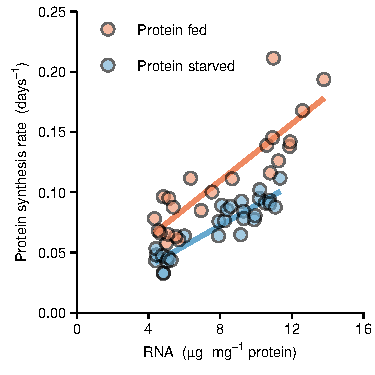
\includegraphics{thesis_files/figure-latex/Millward1973-1} 

}

\caption[Relationship between RNA content and protein synthesis in rat skeletal muscle, data from {[}164{]}]{Relationship between RNA abundance and protein synthesis in rat skeletal muscle. Rats were either starved or fed a protein rich diet stimulating protein synthesis. Data from {[}164{]}.}\label{fig:Millward1973}
\end{figure}
\hypertarget{mtorc1-a-multifaceted-coordinator-of-cell-growth}{%
\subsection{mTORC1 a multifaceted coordinator of cell growth}\label{mtorc1-a-multifaceted-coordinator-of-cell-growth}}

The discovery of an organic compound called rapamycin in the 1960's led to the characterization of a rapamycin sensitive protein involved in cell growth. The protein was later named mechanistic target for rapamycin (mTOR)
{[}169{]}.
mTOR is found in two protein complexes (mTOR complex 1, mTORC1; mTOR complex 2, mTORC2) where primarily mTORC1 has been found to be sensitive to rapamycin treatment.
{[}169{]}.
Bodine \emph{et al.} made a comprehensive characterization of mTORC1-mediated skeletal muscle hypertrophy using rodent models, showing that mTOR activation was essential for load-induced hypertrophy. Additionally, using transfection techniques, they showed that constitutively activated Akt signaling led to hypertrophy in an mTORC1-dependent manner, confirmed with concurrent administration of rapamycin
{[}170{]}.
Further utilizing rapamycin in genetically modified mice where mTOR was made rapamycin-resistant specifically in skeletal muscle cells confirmed that muscle fiber-specific rapamycin-sensitive mTORC1 signaling was needed to induce muscle hypertrophy in response to mechanical loading
{[}171{]}.
This characterization supports previous observational evidence connecting mTORC1 signaling to muscle growth in rats
{[}157{]},
and more recent observations in humans
{[}20, 172{]}.
Administration of rapamycin in humans has also, more directly confirmed that mTORC1 signaling is important for protein synthesis in the acute phase after resistance training (2 hours) and in response to protein ingestion
{[}173, 174{]}.
However, extending the time-frame (up to 24 hours), differences in responses to resistance exercise between rapamycin treatment and control conditions were less pronounced
{[}175{]}.
This could in part be explained by the lower dosage of rapamycin administrated in human compared to animal trials but also indicate rapamycin-insensitive mechanisms controlling translational efficiency
{[}176{]}.

mTORC1 functions as a signaling hub by integrating multiple environmental cues to regulate cellular growth. Among such cues is mechanical stimulation which leads to accumulation of phosphatidic acid in muscle cells
{[}177{]}.
Such activation was shown to be independent of mechanisms upstream of mTORC1 (phosphoinositide 3-kinase (PI3K)/AKT and ERK signaling)
{[}177, 178{]}
but still readily led to mTORC1 activation
{[}177, 178{]}.
In cellular models, phosphatidic acid was shown to interact with mTORC1 on the same site that is targeted by rapamycin
{[}179{]}
indicating a more direct link between mechanical stimulation and mTORC1 activity.
The enzyme primarily responsible for mechanically induced increases of phosphatidic acid has been shown to be diacylglycerol kinase \(\zeta\)
{[}180{]}.

In addition to mechanical stimuli, amino acids and growth factors also stimulate mTORC1 activity and

A well characterized downstream target of mTORC1 is the eIF-4E (eukaryotic translation initiation factor 4E)-bining protein 1 (4E-BP1). Upon activation, 4E-BP1 releases eIF-4E
{[}181{]}
which enables formation of an preinitiation complex and subsequent recruitment of the small ribosomal subunit to mRNA
{[}182{]}.
eEIF-4E-dependent initiation of translation is believed to be rate limiting and thus a control point for protein synthesis.
Interestingly, formation of the preinitiation complex, induced by mTORC1-4E-BP1-mediated release of eIF-4E results in enhanced translation of special classes of mRNAs, containing a 5' structures that does not permit efficient translation
{[}182,183{]}
Among the resulting gene products from such mRNA are growth factors cell cycle regulators such as cyclin D1 and c-Myc as well as ribosomal proteins
{[}169,182{]}.

Downstream of mTORC1 is also S6 kinase 1 (S6K1), present in two isoforms of about 70 and 85 kDa with different localization.
S6K1 was named after its ability to phosphorylate ribosomal protein S6, but has since been shown to have multiple roles
{[}169{]}{]}.

S6K1 depletion in mice results in reduces muscle growth, but does not correlate with reduced rpS6 phosphorylation
{[}184{]}

S6K1 is needed for activation of rDNA transcription through phosphorylation of UBF
{[}185{]}

{[}186{]}

Indeed, mTORC1 affects ribosomal biogenesis through multiple mechanisms including activation of transcriptional programs related to ribosomal biogenesis (mediated through S6K1)
{[}187{]},
selective translation of specific mRNA related to ribosomal biogenesis
{[}188{]}
which in turn stimulates to increased ribosomal RNA transcription, mediated by cyclin D1 abundance and UBF availability
{[}189{]}.

{[}190{]}

{[}158{]}

{[}173{]}
{[}175{]}

\hypertarget{measuring-mtorc1-activity}{%
\subsubsection{Measuring mTORC1 activity}\label{measuring-mtorc1-activity}}

In this context, molecular signatures conveyed by the mechanistic target of rapamycin complex 1 (mTORC1) has been in particular focus. Inhibition of mTORC1 impairs protein synthesis in humans {[}173{]} and activation of its associated downstream target S6 kinase 1 (S6K1) correlates with increases in muscle protein synthesis and subsequent muscle growth

In line with this, surplus {exercise} volume leads to greater phosphorylation of S6K1
{[}20, 21, 22{]} and {is accompanied by increases in }myofibrillar protein synthesis {[}20{]},
fitting the notion that increased training volume provides more pronounced adaptations{ through repeated episodes of increased protein synthesis}.

\hypertarget{ribosomal-biogenesis}{%
\subsection{Ribosomal biogenesis}\label{ribosomal-biogenesis}}

Synthesis of new ribosomes is a highly coordinated, complex and energy demanding process. It involves the synthesis of both ribosomal proteins and the four mature rRNA as well as their assembly into functional ribosomal subunits
{[}191, 192, 193{]}..
The overall role of ribosomal abundance in determining protein synthesis and subsequent cellular and tissue size was briefly mentioned above. In addition to a tight relationship with protein synthesis in mice
{[}164{]}
and cell cultures
{[}165{]}
inhibition of ribosomal RNA (rRNA) transcription and inhibition of its up-stream transcription factors act to diminish muscle cell growth
{[}167,165,193{]}.

Ribosomal accumulation is believed to be determined by the rates of pre-rRNA transcription by RNA polymerase I (Pol I), which in turn is regulated by coordinated assembly of a complex of transcription factors at the rDNA promoter
{[}192{]}.
Specifically, activation of the of the upstream binding factor (UBF) through phosphorylation is needed to initiate transcription
{[}194, 195{]}.
Such activation is at least partly controlled by the mechanosensitive mTOR pathway, with its inhibition being associated with blocked UBF phosphorylation and subsequent rRNA transcription
{[}189, 185{]}.
Interestingly the availability of UBF \emph{per se} has been shown to be a determinant of rRNA transcription
{[}196{]}
through control of rDNA gene activity
{[}197{]}.

{[}198{]}
{[}199{]}

{[}200{]}

Individual response patterns to resistance training, including muscle strength and mass, correlate closely with muscle cell characteristics, measured in both rested-state and acute training-phase conditions
{[}55, 120, 167, 172{]}.

\hypertarget{ribosomal-biogenesis-1}{%
\subsection{Ribosomal biogenesis}\label{ribosomal-biogenesis-1}}

Conversely, inhibition of ribosomal RNA (rRNA) transcription and inhibition of its up-stream transcription factors act to diminish muscle cell growth
{[}167,165,193{]}.

Biosynthesis of novel ribosomes is a complex, highly coordinated and energy demanding process that involves synthesis of both ribosomal proteins and the four mature rRNA transcripts
{[}191, 192, 193{]}.
Ribosomal accumulation is believed to be determined by the rates of pre-rRNA transcription by RNA polymerase I (Pol I), which in turn is regulated by coordinated assembly of a complex of transcription factors at the rDNA promoter
{[}192{]}.
Specifically, activation of the of the upstream binding factor (UBF) through phosphorylation is needed to initiate transcription
{[}194, 195{]}.

{[}195{]}
{[}201{]}

{[}202{]}

{[}152{]}

{[}203{]}

\hypertarget{transcriptional-regulation-of-muscle-mass}{%
\subsection{Transcriptional regulation of muscle mass}\label{transcriptional-regulation-of-muscle-mass}}

{[}204{]}

{[}205{]}

\hypertarget{ribosomal-biogensis-as-a-determinant-of-rt-induced-hypertrophy}{%
\subsubsection{Ribosomal biogensis as a determinant of RT-induced hypertrophy}\label{ribosomal-biogensis-as-a-determinant-of-rt-induced-hypertrophy}}

Resistance exercise is a potent stimuli for rRNA transcription as a single session leads to increases in pre-rRNA
{[}206,207{]}
and repeated bouts lead to accumulation of mature rRNA thus also total RNA and presumably functional ribosomes
{[}206, 208, 168, 167,166, 209, 160{]}.
However, the true time course of ribosomal transcription and accumulation in response to RT remains largely unstudied, with a mere few studies having investigated exercise-induced changes in rRNA over multiple time-points, all of which are either limited to a selected few time-points or a limited time frame.
For example, two consecutive bouts of electrically evoked muscle contractions were associated with increased levels of total RNA, with peak values being observed 72 hrs after the second bout
{[}208{]}.
Using voluntary contractions, peak values were reported after nine sessions, followed by a slight decrease to after 18 sessions {[}209{]},
resembling data from our lab where five sessions of RT led to marked increase in total RNA levels (per-unit muscle tissue), whereby a numerical lowering occurred to after the last training session of the 12 wk interventions (31 sessions).
{[}168{]}.
Interestingly, during the initial phase of RT, total RNA accumulation seems to be volume-dependent, as three sets per exercise in leg exercises led to augmented total RNA and rRNA levels compared to one set per exercise, coinciding with the differences in muscle hypertrophy seen after 12 weeks of RT.
{[}168{]}.
These data suggest that ribosome accumulation reaches a plateau in the early phase of RT and that increases are sensitive to training volume in constant volume protocols.

Recent observations in humans are challenging this view by indicating that translational capacity is a limiting factor for training-induced muscle hypertrophy. First, increased abundances of {ribosomal RNA (rRNA)} in response to resistance training, measured as total RNA per-weight-unit muscle tissue, correlate with muscle hypertrophy {[}166{]}.
In accordance with this, training-induced increases in rRNA are larger in muscle hypertrophy high-responders than in low-responders
{[}167, 210{]}.
Secondly, elderly participants typically show blunted ribosome biogenesis, coinciding with attenuated hypertrophic responses
{[}206, 209{]}.
Collectively, these observations suggest that muscle growth depends at least in part on increased translational capacity, making it a prime candidate for explaining the diverse response patterns seen in resistance training with different volume in different individuals. To date, no study has investigated the association between training volume, ribosome biogenesis and regulation, and gross training adaptations.

.

.

\hypertarget{effects-of-exercise-volume-on-molecular-determinants-of-muscle-growth}{%
\section{Effects of exercise volume on molecular determinants of muscle growth}\label{effects-of-exercise-volume-on-molecular-determinants-of-muscle-growth}}

{[}211{]}

{[}212{]}

\hypertarget{from-training-response}{%
\subsection{From Training response}\label{from-training-response}}

In humans, the biological adaptation to resistance training varies with exercise-training variables such as volume, intensity, rest between repetitions and sets, selection and order of exercises, repetition velocity and frequency of training sessions {[}17{]}.
In addition, genetic and epigenetic disposition and environmental factors play a role in variations in adaptations
{[}58, 213, 69{]}.
As time constraints often hinder participation in exercise training-programs {[}26{]}, numerous studies have searched for the minimal required exercise dose to promote beneficial adaptations. Within-session volume has received particular attention, and although a handful of studies have shown that low-volume training provides similar gains in strength and muscular mass as moderate-volume training
{[}144, 142, 146{]}, meta-analyses conclude in favor of moderate volume protocols {[}23--25,214{]}.
This apparent discrepancy of specific studies to demonstrate benefits of increased training volume is likely due to a combination of small sample sizes and substantial variation in training responses between individuals and experimental groups. In theory, within-participant designs should alleviate these limitations.

\hypertarget{from-rna-seq}{%
\section{From RNA-seq}\label{from-rna-seq}}

Skeletal muscle is a highly adaptable tissue that responds to environmental stress by altering growth rates and differentiation processes. During resistance training, signaling cascades that stimulate muscle plasticity are triggered. Upon repeated exposures, this facilitates growth and a phenotypic shift in a metabolically active direction {[}215{]},
with the opposite happening during inactivity {[}216{]}.
Despite this generalized view, muscle responsiveness and plasticity vary, both in response to different resistance-training protocols {[}168{]} and, perhaps more importantly, between individuals {[}53,\textgreater{} 14{]}.
Selected individuals show a near-complete absence of muscle growth after prolonged resistance training, which markedly reduces the beneficial outcomes of such interventions for muscle function and overall health {[}14, 53{]}.
Currently, little is known about the etiology of this variation. However, it is usually associated with phenotypic traits of skeletal muscle {[}217, 167, 218 {]}, which implies interactions with environmental factors, genetics, epigenetics, and composites of the intra physiological milieu {[}69, 219{]}.
This multifaceted origin makes the training-response-spectrum difficult to study directly, with each of the underlying factors offering limited explanatory value alone {[}58{]}.
Instead, a more indirect approach is necessary, whereby the combined effects of the factors are targeted by studying global patterns of mRNA, protein expression, and skeletal muscle biology.

Previous studies have investigated transcriptome responses to acute resistance exercise {[}220, 119, 221{]}
and chronic resistance training {[}222, 223, 119, 224, 220, 120{]},
as well as described associations between transcriptome characteristics and degrees of muscle growth {[}120, 225{]},
and function {[}226, 227{]}.
Whereas these studies have merited interesting findings, they lack clear coherences in terms of differential expression events, even for classical exercise-inducible genes such as PGC1\(\alpha\) {[}228{]}.
This lack of clear coherence is potentially due to a combination of issues such as differences in study design and methods for synthesis and analysis of transcriptome data. First, biologically founded variability can be attributed to differences in exercise protocols (e.g., differences in exercise-volume or intensity). This makes it difficult to discern a general transcriptome exercise response, as training variables are not standardized between studies. Biological heterogeneity is also caused by differences between research participants, affecting signal-to-noise ratios and making it difficult to discern the effects of single independent factors such as training variables. Design stage decisions such as the use of within-participant designs {[}168, 229{]} are likely to reduce this variation and to provide transcriptome data with increased biological meaningfulness. Second, technical variability can be attributed to decisions made during the bioinformatical treatment of data. As described by Concea \emph{et al.}, there is no optimal pipeline for sequencing technology as new tools keep evolving and emerging, different tools should be explored to an optimum pipeline for the specific type of data {[}230{]}.
To exploit the potential of any study design, there is a need for identifying an appropriate pipeline for transcriptome analyses to ensure a biologically valid interpretation of data. This entails identifying potential violations of common assumptions caused by the experimental model at hand, relating to, for example, data normalization {[}231, 232{]}.

For transcriptome data to provide adequate biological information about a given experimental set-up, numerous bioinformatic steps need to be adopted in a customized manner {[}230, 233{]}.
Of these steps, data normalization is particularly decisive {[}232{]},
as it aims to transform naïve transcript counts into biologically meaningful results. This essentially means expressing them as \emph{per}-cell abundances {[}234{]}.
For most experimental models, this is equivalent to providing transcript-to-total RNA ratios, given the fulfillment of the assumption that total RNA levels remain stable between conditions on a per-unit-cell or per-unit-tissue basis {[}234{]}.
In cell models that exhibit high degrees of plasticity, gene expression events result in increased amounts of total RNA and mRNA transcripts per cell {[}235{]}, specifically violating the assumption that most genes are not differentially expressed {[}234, 231{]}.
We are not aware of any study that has addressed the need to account for such perspectives during transcriptome analyses of skeletal muscle subjected to mechanical stress, such as resistance training. Indeed, this assumption can be expected to be violated, as total RNA content increases markedly on a per-unit-weight basis {[}168{]}, with potential global changes also occurring for the mRNA pool, though this remains unknown. The extent to which total RNA, and therefore ribosomal RNA, increases, coincides with the increase in muscle mass {[}168,167{]}, underlining its importance for cellular growth but also its inevitable presence as a potential confounding factor in RNA sequencing experiments.

\hypertarget{from-tr10}{%
\section{From tr10}\label{from-tr10}}

Skeletal muscle is a critical target for interventions that promotes health across the lifespan {[}11{]},
with resistance training (RT) being the advocated remedy.\\
Prolonged RT leads to changes in the balance between muscle protein breakdown and synthesis, with one bout of resistance exercise acutely increasing protein synthesis for up to 48 hrs after exercise {[}150{]},
with subsequent repeated bouts leading to accumulation of muscle protein over time
{[}236,237{]}.

\hypertarget{aims}{%
\chapter{Aims}\label{aims}}

The primary aim of this thesis was to relate the adaptive response to resistance training with low- and moderate-volume to skeletal-muscle characteristics in previously untrained individuals. The key question was whether manipulation of exercise-volume will have diverse effects in different individuals related to muscular intrinsic characteristics. A further aim was to characterize exercise-volume dependence in muscle molecular characteristics and determine a time course profile of markers of ribosomal biogenesis in response to resistance training. Based on these aims, the objectives of the present thesis were;
\begin{itemize}
\tightlist
\item
  to relate skeletal muscle and systemic characteristics to benefit of moderate- compared to low-volume resistance training;
\item
  To determine volume-dependence in molecular networks related to muscle growth and remodeling in response to resistance training
\item
  To determine a time course of markers related to ribosome biogenesis in the early phase of resistance training.
\end{itemize}
\hypertarget{methods}{%
\chapter{Methods}\label{methods}}

\hypertarget{study-protocols-and-participants}{%
\section{Study protocols and participants}\label{study-protocols-and-participants}}

Study I was designed to examine effects of low- (single-set per exercise) and moderate-volume (three sets per exercise, multiple-sets) on
responses to acute exercise and long-term training within participants.
A schematic overview of Study I can be seen in Figure \ref{fig:study1-overview}.
Prior to the training intervention, participants reported to the laboratory for bilateral baseline muscle biopsies (\emph{m. vastus lateralis}).
Bilateral muscle biopsies were additionally sampled prior to, and 60 minutes after the fifth training session as well as after the intervention (Figure \ref{fig:study1-overview}).
Assessments of muscle strength (isokinetic and isometric knee extension torque as well as one repetition maximum) were performed twice at baseline and further measured in weeks 3, 5, 9 and after the intervention (Figure \ref{fig:study1-overview}).
Body composition measurements (magnetic resonance imaging and dual-energy X-ray absorptiometry) were performed at baseline and after the intervention.
\begin{figure}

{\centering 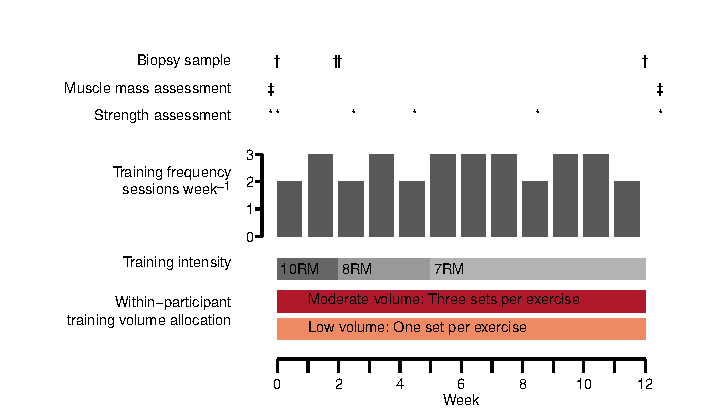
\includegraphics{thesis_files/figure-latex/study1-overview-1} 

}

\caption[Study I, schematic overview]{Schematic representation of Study I, see text for details.  }\label{fig:study1-overview}
\end{figure}
Study II was designed to study the effects of resistance training \emph{per se} and effects of variable compared to constant inter-session volume on selected markers related to ribosome biogenesis.
Participants were therefore recruited to an experimental group (\emph{n =} 11) and a non-training control group (\emph{n =} 8).
An overview of Study II can be seen in Figure \ref{fig:study2-overview}.
Baseline muscle strength (isokinetic and isometric knee-extension torque) was assessed during three initial visits to the laboratory, with the last baseline-assessment performed at least seven days prior to the first biopsy sampling. Follow-up measures of muscle strength in the experimental group were completed three and nine days after the last training session.
Muscle thickness (\emph{m. vastus lateralis}) was measured bilaterally prior to the study as well as two and eight days after the last training session in the experimental group.
Muscle biopsies were sampled bilaterally prior to any training, 48 hours after the first, fourth, fifth, eighth, ninth and twelfth session as well as eight days after the twelfth session (Figure \ref{fig:study2-overview}).
The control group in Study II performed the same initial assessments as the experimental group. Muscle thickness was again assessed after a control period of 2-4 weeks.
Follow-up muscle biopsies were sampled from one leg 48 hours after the first biopsy as well as after the control period. Follow-up strength assessments were performed 24 hours after the last biopsy.
\begin{figure}

{\centering 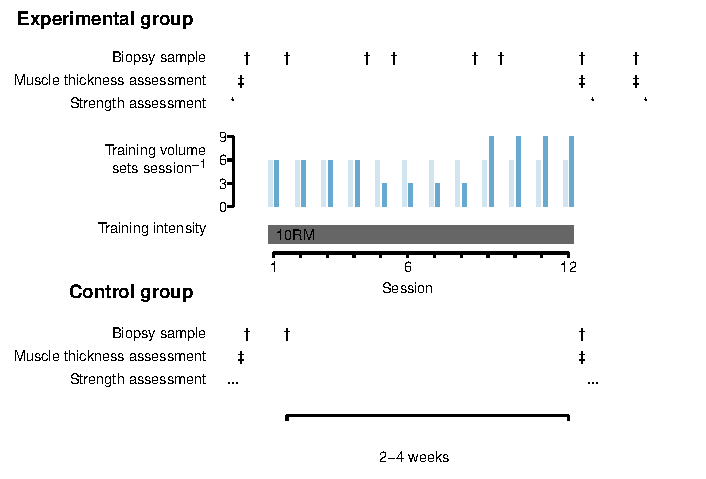
\includegraphics{thesis_files/figure-latex/study2-overview-1} 

}

\caption[Study II, schematic overview]{Schematic representation of Study II, see text for details.  }\label{fig:study2-overview}
\end{figure}
Recruitment to both studies was done through advertising and word of mouth, primarily at Lillehammer University College/Inland University of Applied Sciences. Potential participants were interviewed and matched against inclusion and exclusion criteria. During initial interviews, participants were informed of the study design and time requirements. Participants were also informed about potential risks and sources of discomfort associated with the study prior to giving their informed consent.

To be eligible for participation in both studies, participants had to be young (Study I age 18-40; Study II 18-35) and non-smoking. Both men and women were considered for participation. Exclusion criteria included a training history of more than one weekly session during the last 12 (Study I) or six (Study II) months leading up to the study. Participants were also screened for intolerance to local anesthetic, current or previous injuries affecting their ability to perform resistance training, self-reported symptoms or history of disease, intake of medications or supplements with known effects on adaptations to training.
Participant characteristics for both studies are shown in Table
\ref{tab:characteristics-table}.

Forty-one healthy individuals were recruited and 34 of these completed
at least 85\% of the prescribed sessions and were thus included in
subsequent data analyses. Reasons for not completing the trial included
injury not related to the study (\emph{n =} 1), pain or discomfort during
exercises (\emph{n =} 5) and non-adherence to the study protocol. There were
no systematic differences in characteristics between participants included in or
excluded from data analysis in Study I.

Prior to the study, all participants reported that they previously had been engaged in sporting activities. At enrollment, twenty participants reported regular physical activities ranging from once every other week to four times per week. Ten participants reported performing resistance-type exercise at the time of enrollment limited to no more than once a week.
\begin{table}

\caption{\label{tab:characteristics-table}Participant characteristics}
\centering
\fontsize{7}{9}\selectfont
\begin{tabular}[t]{llllllll}
\toprule
  &   & Sex & Age (years) & Stature
(cm) & Mass (kg) & Fat mass (\%) & Lean mass (\%)\\
\midrule
 &  & Female & 22.0 (1.3) & 168 (7) & 64.4 (10.4) & 34.1 (5.6) & 64.3 (6.2)\\
\cmidrule{3-8}
 & \multirow{-2}{*}{\raggedright\arraybackslash Included} & Male & 23.6 (4.1) & 183 (6) & 75.8 (10.7) & 20.4 (6.0) & 79.3 (5.0)\\
\cmidrule{2-8}
 &  & Female & 22.9 (1.6) & 166 (8) & 64.6 (9.7) & 28.8 (8.7) & 68.6 (9.1)\\
\cmidrule{3-8}
\multirow{-4}{*}{\raggedright\arraybackslash Study I} & \multirow{-2}{*}{\raggedright\arraybackslash Excluded} & Male & 24.3 (1.5) & 189 (5) & 88.2 (22.4) & 24.3 (15.3) & 76.8 (12.7)\\
\cmidrule{1-8}
 &  & Female & 23.4 (2.9) & 168 (8) & 64.0 (9.2) & 30.8 (7.1) & 65.5 (6.8)\\
\cmidrule{3-8}
 & \multirow{-2}{*}{\raggedright\arraybackslash Training} & Male & 25.7 (5.8) & 177 (3) & 77.5 (8.0) & 25.3 (3.9) & 71.3 (2.4)\\
\cmidrule{2-8}
 &  & Female & 24.1 (3.5) & 166 (4) & 63.8 (0.6) & 30.5 (6.4) & 66.3 (5.2)\\
\cmidrule{3-8}
\multirow{-4}{*}{\raggedright\arraybackslash Study II} & \multirow{-2}{*}{\raggedright\arraybackslash Control} & Male & 25.5 (5.5) & 182 (5) & 76.5 (7.7) & 18.2 (5.1) & 78.7 (4.2)\\
\bottomrule
\multicolumn{8}{l}{\rule{0pt}{1em}Data are means and (SD)}\\
\end{tabular}
\end{table}
\hypertarget{resistance-training-interventions}{%
\section{Resistance training interventions}\label{resistance-training-interventions}}

Each training session started with a light, standardized warm-up (5 min
ergometer cycling and 10 repetitions each of push-ups, sit-ups,
back-extensions and squats). Before each exercise in the main program,
one set of 10 repetitions were performed in the specific exercise with
approximately 50\% of 1RM.

Studies were fully or partially performed as within-participant studies
as each participant had their legs assigned to different training
conditions (not including the control group in Study II). Allocation was
performed after enrollment where each participant had their legs
randomized to either low- or moderate volume (Study I, see Figure \ref{fig:study1-overview}), or variable or constant volume (Study II).

In Study I, the low-volume protocol consisted of a single set of each
exercise and the moderate-volume consisted of three sets per exercise.
Three unilateral leg exercises were used (leg press, leg curl and knee
extension). The moderate volume-leg commenced all sessions and the low
volume-leg performed a single set of each exercise in the rest between
second and third set of the moderate volume training protocol.

In Study II, only unilateral knee-extension was performed in an effort
to concentrate the stimulus to the quadriceps
muscles. The constant-volume leg performed six sets
of 10RM throughout the study and variable leg performed six sets in
session one to four, three sets in session five to eight and nine sets
in session nine to twelve with same relative intensity (see Figure \ref{fig:study2-overview}).

\hypertarget{muscle-strength-assessments}{%
\section{Muscle strength assessments}\label{muscle-strength-assessments}}

\hypertarget{isokinetic-and-isometric-maximal-torque}{%
\subsection{Isokinetic and isometric maximal torque}\label{isokinetic-and-isometric-maximal-torque}}

Maximal isokinetic and isometric unilateral knee-extension strength was determined by use of a dynamometer (Study I: Cybex 6000, Cybex International, Medway USA; Study II: Humac Norm, CSMi, Stoughton, MA, USA).
After a brief warm-up (5 min ergometer cycling, RPE 12-14), participants were secured at the hip and shoulders in the dynamometer with the knee joint aligned to its rotation axis.
Individual settings were recorded and used in subsequent measurements.
Participants were familiarized with the test protocol by performing three sub-maximal efforts at each angular speed.
In Study I, three angular velocities were used to determine isokinetic torque (60\(^{\circ}\), 120\(^{\circ}\) and 240\(^{\circ} ~\times\) sec\(^{-1}\)), in Study II an angular velocity of 90\(^{\circ} ~\times\) sec\(^{-1}\) was used for this purpose.
In Study I, participants performed two attempts at 60\(^{\circ} ~\times\) sec\(^{-1}\) and three attempts at 120 and 240\(^{\circ}~\times\) sec\(^{-1}\).
In Study II, three attempts were made at the designated angular velocity.
In both studies, attempts within each angular speed were performed in immediate succession.
After isokinetic testing, the lever was fixed at 30\(^{\circ}\) (full extension \(=90^{\circ}\)), participants were instructed push with maximal effort for 5 seconds and the maximal isometric torque was recorded.
Two attempts were made for maximal isometric torque in Study I and a single attempt was made in Study II.
Sixty seconds of restitution was given between each measurement in both studies with the exception of between isometric contractions in Study I where a 30 second restitution period was used.

In subsequent assessment sessions, the first measurement was performed on alternate legs.
In Study II, the dynamometer allowed for participants to remain seated for assessments of both legs. This was not possible in Study I as the measurement system required participants to be re-seated for assessment of the contra-lateral leg.

\hypertarget{one-repetition-maximum}{%
\subsection{One-repetition maximum}\label{one-repetition-maximum}}

One repetition-maximum (1RM) was assessed in unilateral leg-press and knee-extension in Study I.
Each exercise was assessed after a specific warm-up (ten, six and three repetitions at \(50\), 75 and \(85\%\) of the anticipated maximum). Attempts were made with increasing resistance (four to six attempts) and one repetition maximum was defined as the highest resistance successfully lifted through the full range of motion.

\hypertarget{strength-assessment-frequency-and-statistics}{%
\subsection{Strength assessment frequency (and statistics)}\label{strength-assessment-frequency-and-statistics}}

In Study I, maximal values from each assessment and time-point was used in statistical analyses including two separate assessments at baseline, separated by at least four days. Strength was determined

In Study II, the maximal value from all successful attempts were used in statistical analyses with unsuccessful attempts identified based on obvious misinterpretation of instructions or failure to reach maximal subjective effort.\\
Strength assessments were separated by at least 48 hours from preceding training sessions.

At baseline, 1RM, isokinetic and isometric strength assessments were performed twice, separated by at least four days. The maximum value achieved for each of the tests was used in subsequent analysis. Strength tests were separated by at least 48 hours from preceeding training sessions. A combined measure of muscle strength was calculated as the average of all tests (1RM, isometric and isokinetic), wherein each test modality was given equal weight. A subset of the participants (n=18) performed strength assessment during the course of the study (at week two, five and nine). For the remaining participants, ordinary training sessions were prioritised when participants missed training or testing due to illness or scheduling difficulties.

Muscle strength was assessed as maximal voluntary isokinetic (90° sec-1) and isometric (60° angle, fully extended leg 0°) knee extension torque. After a brief warm-up (5-min cycling, RPE 12-14), participants were seated and secured in the individually adjusted dynamometer. Participants were instructed to gradually increase their effort during three warm-up repetitions (50, 60 and, 70\% of subjective maximal effort). After a 30-sec restitution period participants were instructed to perform three repetitions with maximal effort in the concentric phase. Sixty seconds after the isokinetic test the lever automatically moved to a 60° angle and participants were instructed to push against the lever enough to see feedback from the visual feedback system. After an additional 15-sec restitution period, participants were instructed to push against the lever with maximal effort. Within the same assessment session, participants remained seated in the dynamometer for measurement perfomed on both legs. The first measurement was alternated between legs every other session. For statistical treatment of the data, all successful attempts were used. The last strength assessment at baseline was performed at least seven days prior to the first biopsy sampling. At least one of the baseline strength tests was performed on separate day with two sessions allowed to be perform on the same day with a short rest between assessments. Post training assessments were performed 48 hours and eight days after the last session.

\hypertarget{measures-of-muscle-mass}{%
\section{Measures of muscle mass}\label{measures-of-muscle-mass}}

In Study I muscle mass was measured by magnetic resonance imaging (MRI)
and dual energy X-ray absorptiometry (DXA) prior to and after the
intervention. Both MRI and DXA measurements were completed during the
same visit to the laboratory. Participants were instructed to refrain
from strenuous physical activity during the last 48 h leading up to the
measurements. The post-training measurements were completed at least 48
h after the last strength testing session. Participants were asked to
refrain from food consumption during 2 h leading up to the measurements.

MRI images were obtained from the mid-thigh and analyzed by the same
investigator blinded for time (pre- and post-training) and condition
(low- and moderate-volume). Multiple images were used to estimate the
cross-sectional area of the extensor muscles at the same distance from
the knee-joint.

See figure

In Study II, m. vastus lateralis muscle thickness was measured by B-mode ultrasonography (SmartUs EXT-1M, Telemed, Vilnius, Lithuania) using a 39 mm 12 MHz, linear array probe. At least three images were captured for each leg per time-point. Between each image acquisition the probe was relocated to the same position where on the skin and subsequently marked on a soft transparent plastic sheet superimposed on the thigh.

Muscle thickness of m. vastus lateralis and m. rectus femoris were measured using Transverse images were obtained \(\sim\) 60 \% distally from the trochanter major towards the femoral lateral epicondyle. Landmarks such as moles and scars were also marked on the plastic sheet for relocation of the scanned areas during post-training measurements. During analysis, pre and post images from the same participant were analyzed consecutively using the Fiji software,66 and by two independent researchers. The average muscle thickness of the three images captured per muscle was used for further analyses.

For determination of body composition participants were scanned using DXA (Lunar Prodigy densitometer, GE Healthcare, Madison, WI, USA) with the standard scanning mode (13-25 cm). Participants were lying supine within the scanning bed reference lines, with a strap secured around the ankles to ensure a standardized body position in each scan. The scans were conducted with participants in a fasted state between 07.00-10.00 AM, with empty bladder and wearing only under-wear. Prior to each scan, a phantom scan was run to prevent baseline drifting from affecting analyses. The same technician was used at each time point. Analyses was performed using GE enCORE version 17.0 software (GE Healthcare). Region of interest was customized for covering upper thigh, marked with a sqaure from pubic symphysis to lateral part of tuberculum major, and distal to art. genu.

Muscle thickness (MT) was measured using a B-mode ultra sound unit (SmartUS EXT-1M, Telemed, Vilnius, Lithuania). Participants lay supine in a relaxed position for 20 min before assessments, with their feet strapped in a standardized position. A mark was set on the line 60\% of the distance between Spinia Iliac Anterior Superior and the lateral femur condyle. MT of \emph{m.vastus lateralis} was measured applying a water-soluble transmission gel (Aquasonic 100 Ultrasound Transmission Gel; Parker Laboratories Inc., Fairfield, NJ, USA), and a 39 mm 12 MHz ultrasound probe was placed perpendicular to the site of interest without pressing the skin. When the quality of the image was satisfactory, evident as distinct upper and lower muscle fascia, three images were captured, where the probe was relocated to the same position between each image. Position of the probe was marked on the skin and subsequently marked on a transparent paper to ensure similar probe placement for both the right and left \emph{m.vastus lateralis} at subsequent assessments. Analyses were done in ImageJ Fiji {[}238{]} with images cropped and coded to ensure blinding of the assessor.

\hypertarget{muscle-tissue-sampling-and-preparations-for-downstream-analyses}{%
\section{Muscle tissue sampling and preparations for downstream analyses}\label{muscle-tissue-sampling-and-preparations-for-downstream-analyses}}

Muscle samples were obtained under local anesthesia (Study I, Xylocaine,
\SI{10}{\mg\per\ml} with adrenalin \SI{5}{\micro\gram\per\ml},
AstraZeneca, Oslo, Norway; Study II, Lidocaine Mylan,
\SI{10}{\mg\per\ml}, Mylan Ireland Ltd, Ireland) with a fine needle
(12-14 gauge; Universal-plus, Medax, Italy) operated with a
spring-loaded instrument (Bard Magnum, Bard Norway AS, Norway). Sampling
was performed as previously described
{[}239{]}, with
modifications. Anesthesia was injected in the subcutaneous tissue with
care taken not to inject anesthesia into the muscle itself. Following
pilot experiments we decided not to use an insertion cannula as
described in {[}239{]} as the biopsy needle itself could be used to
puncture the skin and muscle fascia. This also resulted in less
discomfort. Several passes through the same skin puncture was made to
obtain sufficient material for downstream analyses. A smaller needle (14
vs.~12 gauge) was used to further minimize discomfort in Study II where
more biopsies were sampled over a shorter time span, with exception from
when material was used for immunohistochemistry. The first biopsy was
sampled at one third of the distance between the patella to the
\emph{anterior superior iliac spinae} with subsequent biopsies sampled
\(\sim\)\SI{2}{cm} proximal to previous samples. In Study II, samples
obtained more than one week apart were sampled with closer proximity and
distally from previous samples but never at previous sampling sites.

The micro biopsy technique produces smaller samples compared to other
biopsy techniques
{[}240{]}, and thus
requires several passes to produce sufficient material for multiple
downstream experiments. However, reports confirms that the micro biopsy
technique is comparable to the traditionally used Bergström technique in
several measures of muscle characteristics at the same time as being
well tolerated {[}239,241{]}. Any reported differences in fiber type
distributions between sampling techniques have been suggested relating
to differences in sampling depth {[}241,242{]}.

For determination of fiber type distributions, a threshold of 200-300
fibers has been suggested as a suitable sample size per specimen as more
fibers does not reduce the variation between dupliacte samples
{[}243{]}.
In Study I, one or several pieces of muscle (total weight
\(\sim\)\SI{15}{mg}) were chosen per sampling for analysis of fiber type
distributions (described in detail below). The total number of fibers
were counted from these specimens (Figure ref fig). Using an average of
fibers from the first sampling time point the between leg coefficient of
variation was determined to 14\% for Type I fibers and 11.3 for type II
fibers. The between leg variation in Type I fibers is similar to what
has been previously reported\ldots{}

\hypertarget{total-rna-extraction}{%
\subsubsection{Total RNA extraction}\label{total-rna-extraction}}

Total-RNA was extracted from frozen muscle samples with weights measured at collection using a protocol modified from
{[}244{]}
using Trizol reagent (Life Technologies).
Muscle tissue was homogenized in \SI{300}{ul} Trizol with mechanical disruption achieved by Zirconium Oxide Beads (0.5 mm, Next Advance, Inc., New York, USA) and a bead mill (Bullet blender, Next Advance). External, non-mammalian RNA (Lambda PolyA External Standard Kit, Takara Bio Europe, Saint-Germain-en-Laye, France) was added with the initial volume of Trizol to enable per-weight normalization in subsequent analyses. After homogenization, additional Trizol was added to a total volume of \SI{1}{ml}. Phase separation was achieved by centrifugation after addition of chloroform (\SI{200}{ul}). The upper phase (\SI{400}{ul} in Study I; \SI{450}{ul} in Study II) was transferred to a fresh tube and RNA was precipitated using isopropanol (\SI{500}{ul}). After incubation (10 min, room-temperature) and centrifugation (12000 g, 10 min at 4\(^{\circ}\)C) the resulting RNA pellet was washed three times in chilled 75\% ethanol.

As previously mentioned, to minimize discomfort with a larger number of biopsies sampled over a short time, a smaller needle was used for most biopsies in Study II. This generally led to a less tissue used for RNA extractions (Figure XX).

\hypertarget{protein-extraction-immunoblotting}{%
\subsubsection{Protein extraction immunoblotting}\label{protein-extraction-immunoblotting}}

Aliquots of muscle-tissue (approximately 25 mg wet weight) were homogenised using a plastic pestle in ice-cold lysis buffer (2 mM HEPES pH 7.4, 1 mM EDTA, 5 mM EGTA, 10 mM MgCl\textsubscript{2}, 1\(\%\) Triton X-100) spiked with protease and phosphatase inhibitors (Halt, Thermo Fischer Scientific, Life Technologies AS, Oslo Norway), incubated at \(4^{\circ}\) for 1 hr and centrifuged for 10 min at 10 000 g and 4\(^{\circ}\)C, after which the supernatants were collected.
Total protein concentrations were determined on a 1:10 dilution (Pierce Detergent Compatible Bradford Assay Reagent, Thermo Fischer Scientific). The remaining supernatant was diluted to 1.5 \(\mu g \times \mu l^{-1}\) total protein in lysis buffer and 4X Laemmli sample buffer (Bio-Rad Laboratories AB, Oslo Norway) containing 2-Mercaptoethanol.
Samples were heated to 95\(^{\circ}\)C for 5 min and stored at -20\(^{\circ}\)C until further processing.
During analyses, protein samples (20 \(\mu g\) of total protein) were separated at 300 V for 30 min using 4-20\% gels (Criterion TGX, Bio-Rad), followed by wet transfer to PVDF membranes (0.2 \(\mu m\) Immun-Blot, Bio-Rad) at 300 mA for 3 h.
Gel electrophoresis and protein transfer were performed at 4\(^{\circ}\)C.
Membranes were then stained using a reversible total protein stain (Pierce Reversible Protein Stain, ThermoFischer Scientific) to ensure appropriate protein transfer.
Primary antibodies were purchased from Cell Signaling Technology (Leiden, The Netherlands): mTOR (mTOR\textsuperscript{Ser2448}: \#5536; pan: \#4517), S6 kinase 1 (p85 S6K1\textsuperscript{Thr412}: \#9206; p70 S6K1\textsuperscript{Thr389}: \#9234; pan: \#2708), ribosomal protein S6 (rpS6\textsuperscript{Ser235/236}: \#4858; pan: \#2317).
Membranes were blocked for 2 h in tris-buffered saline (TBS, 20 mM Tris, 150 mM NaCl) containing \(3\%\) bovine serum albumin and \(0.1\%\) Tween-20, followed by over-night incubation with primary antibodies targeting either the phosphorylated or non-phosphorylated epitope diluted in blocking buffer, followed by 2 h incubation with secondary horseradish peroxidase-conjugated antibodies diluted in TBS containing 0.1\% Tween-20 and \(5\%\) skimmed milk. Membranes were washed in TBS containing \(0.1\%\) Tween-20 for 6 \(\times\) 5 min after incubation with primary antibody, and for 8 \(\times\) 5 min after incubation with secondary antibodies. For rpS6 and mTOR antibodies, following chemiluminescent detection (SuperSignal™ West Femto Maximum Sensitivity Substrate, ThermoFischer Scientific), membranes were incubated with hydrogen peroxide (15 min, 37\(^{\circ}\)C) to inactivate the horseradish peroxidase (HRP), as described by Sennepin \emph{et al.} {[}245{]}, followed by over-night incubation with primary or secondary antibodies as described above. If the phosphorylated epitope was targeted during the first incubation, antibodies for the non-phosphorylated epitope were used in the second and vice versa. HRP inactivation did not affect the phosphospecific to non-phosphorylated signal ratios. Importantly, as this technique did not involve removing the first primary antibody, antibodies from different hosts (mouse or rabbit) were used for phosphorylated and non-phosphorylated epitopes respectively. As the antibody targeting p70 S6K1\textsuperscript{Thr389} had the same host as the pan-antibody, total-protein was used to normalise chemiluminescent signals. All incubation and washing steps were performed at \(4^{\circ}\)C using an automated membrane processor (BlotCycler, Precision Biosystems, Mansfield, MA, USA), except for p70 S6K1 experiments, which were performed by hand at room temperature with incubations at \(4^{\circ}\)C. For mTOR and rpS6, total-protein and chemiluminescence quantification was calculated as the mean value of two separate experiments. S6K1 was quantified once for each phospho-specific antibody. Total-protein content was quantified using ImageJ {[}246{]}, and was defined as the mean grey value of the whole well with between-well values subtracted as background. Chemiluminescence signals were quantified using Image Studio Lite (LI-COR Biotechnology, Lincoln, Nebraska USA).

Protein was extracted from Trizol preparations according to manufacturers instructions and {[}247{]} with modifications. The remaining aqueous phase was removed and DNA was precipitated by the addition of \SI{300}{ul} of absolute ethanol followed by gentle centrifugation (2000 g, 5 min at room temperature). An aliquot of the phenol-ethanol phase, corresponding to \textasciitilde1.75 mg of tissue, was transferred to to a fresh tube. After addition of at least two volumes of isopropanol and incubation (10 min at room temperature), samples were centrifuged (7500 g, 10 min 4\(^{\circ}\)C) and a pellet formed. The pellet was washed three times in 95\% ethanol with each wash separated by centrifugation (5000g, 5 min at room temperature). After the last wash all liquid was removed and \SI{45}{ul} of Kopec buffer {[}247{]} was added (5\% SDS, 10 mM Tris, 140 mM NaCl and 20 mM EDTA, pH 8; containing protease and phosphatase inhibitors). Pellets were incubated at 50\(^{\circ}\)C for three hours after which the majority of samples were dissolved. Any undissolved material was sedimented by centrifugation (10000 g, 10 min at room temperature). Protein concentrations were measured (Pierce Detergent Compatible Bradford Assay, ThermoFisher Scientific). Sample were normalized in 4X Laemmli buffer (Bio-Rad Norway AS, Oslo, Norway), boiled (95\(^{\circ}\)C, 5 min) and stored at -20\(^{\circ}\)C before later use.

\hypertarget{rna-analysis}{%
\section{RNA analysis}\label{rna-analysis}}

Complementary DNA (cDNA) was synthesized in technical duplicates from 500 ng of total RNA using random hexemer and anchored Oligo-dT primers (Thermo Fisher Scientific) together with Superscript IV (Thermo Fisher Scientific) according to manufacturer's instruction. qPCR reactions were performed with diluted cDNA (2 ul, 1:25 dilution), a SYBR-green based commercial master mix (PowerUp™ SYBR™ Green Master Mix, Thermo Fisher) and, target-specific primers (500 nM) in 10ul reaction volumes using a real-time detection system (QuantStudio 5 Real-Time PCR System, Thermo Fisher Scientific). Fast cycling was used (1 sec denaturing, 30 sec annealing) after UNG (2 min, 50\(^{\circ}\)C) and polymerase (2 min, 95°C) activation. Melt curves were collected from all reactions to confirm single product amplification. Primers were further evaluated by agarose gel electrophoresis which confirmed primer sizes and non-template control experiments confirming no amplification without template. Primer sequences and their respective average performances are shown in Table 2.

Approximately 25 \(mg\) of wet muscle-tissue was homogenised in a total volume of 1 ml of TRIzol reagent (Invitrogen, Life technologies AS, Oslo, Norway) using 0.5 mm RNase-free Zirconium Oxide beads and a bead homogeniser (Bullet Blender, Next Advanced, Averill Park, NY, USA) according to the manufacturer's instructions.
In order to enable analysis of target gene-expression per-unit tissue weight, an exogenous RNA control (\(\lambda\) polyA External Standard Kit, Takara Bio Inc, Shiga, Japan) was added at a fixed amount (\(0.04 ~ng \times ml^{-1}\) of Trizol reagent) per extraction prior to homogenisation, as previously described
{[}248, 249{]}.
Following phase-separation, 400 \(\mu l\) of the upper phase was transferred to a fresh tube and RNA was precipitated using isopropanol.
The resulting RNA pellet was washed three times with 70\% EtOH and finally eluted in TE buffer.
RNA quantity and purity was evaluated using a spectrophotometer, all samples had a 260/280 \(nm\) ratio \textgreater{} 1.95. RNA was stored at -80\(^{\circ}\)C until further processing. In the analysis of total RNA content per-unit tissue weight, one sample was excluded prior to analysis due to negative deviation from the expected value based on the relationship between sample weight and RNA content suggesting sample loss in washing steps.
RNA integrity was assessed by capillary electrophoresis (Experion Automated Electrophoresis Station using RNA StdSens Assay, Bio-Rad) with average integrity scores (RQI)
Five-hundred nanograms of RNA were reverse transcribed using anchored Oligo-dT, random hexamer primers (Thermo Scientific) and SuperScript IV Reverse Transcriptase (Invitrogen) according to manufacturer's instructions.
All samples were reverse transcribed in duplicates and diluted 1:50 prior to real-time polymerase chain reaction (qPCR).
qPCR reactions were run on a fast-cycling real-time detection system (Applied Biosystems 7500 fast Real-Time PCR Systems, Life technologies AS), with a total volume of 10 \(\mu l\), containing 2 \(\mu l\) of cDNA, specific primers (0.5 \(\mu M\) final concentration) and a commercial master mix (2X SYBR Select Master Mix, Applied Biosystems, Life technologies AS). qPCR reactions consisted of 40 cycles (three seconds 95\(^{\circ}\)C denaturing and 30 seconds 60\(^{\circ}\)C annealing).
Melt-curve analyses were performed for all reactions to verify single-product amplification. Gene-specific primers were designed for all targets using Primer-BLAST {[}250{]} and Primer3Plus {[}251{]} and ordered from Thermo Scientific, except for the external RNA control, for which primers were supplied with the kit.
Raw fluorescence data was exported from the platform specific software and amplification curves were modelled with a best-fit sigmoidal model using the qpcR-package {[}252{]} written for R {[}\textbf{R-base?}{]}. Threshold cycles (Ct) were estimated from the models by the second-derivate maximum method with technical duplicates modelled independently.
Amplification efficiencies were estimated for every reaction {[}as described by 253,implemented in 252{]}. For every primer pair, mean amplification efficiencies (\(E\)) were utilised to transform data to the linear scale using \(E^{-Ct}\). Primer sequences and primer characteristics (i.e.~average primer efficiencies and Ct values) are presented in Table 2. Gene expression data was log-transformed prior to statistical analysis. As Ct-values, but not efficiencies are related to RNA integrity {[}254{]}, RQI scores were used in the statistical treatment of qPCR data to control for potential degradation effects on a by target basis (see below).

\hypertarget{hormonal-measurements}{%
\subsection{Hormonal measurements}\label{hormonal-measurements}}

Hormone analyses were performed on blood samples collected at five time points: alongside muscle biopsies (Figure 1, four sampling events) and 10 minutes after completion of the fifth training session. Samples were drawn from the antecubital vein into serum-separating tubes and kept at room temperature for 30 min before centrifugation (1500 g, 10 min). Serum was immediately aliquoted and stored at -80\(^{\circ}\)C until further processing. Serum concentrations of total testosterone, cortisol, growth hormone and insulin-like growth-factor 1 (IGF-1) were measured on an Immulite 1000 analyzer, using kits from the Immulite Immunoassay System menu (Siemens Medical Solutions Diagnostics, NY, USA), performed according to manufacturer's protocols. Serum Vitamin D (S-25-OH-D) levels were measured in samples collected before and after the intervention using a electrochemiluminescence immunoassay (Roche Cobas Vitamin D total assay, Roche Diagnostics GmbH., Mannheim, Germany) using automated instrumentation (Roche Cobas 6000's module e601, Roche Diagnostics GmbH., Mannheim, Germany).

\hypertarget{statistics-and-data-analysis}{%
\section{Statistics and data analysis}\label{statistics-and-data-analysis}}

In Study I, an \emph{a priori} sample-size calculations (\(\beta=20\%\), \(\alpha=5\%\)) indicated that 40 participants was sufficient to detect \(\sim\) 3\% and 5\%-point differences between volume conditions in primary outcomes, training induced changes in muscle cross-sectional area and maximal voluntary strength respectively. Sample-size calculations were based on assumed differences between volume condition corresponding to effect sizes of 0.47-0.51, as estimated from previous studies {[}145,146{]}.

In Study II, an initial sample size calculation was made based on a best case scenario. Data from Brook et al. {[}237{]} indicated that a within-participant differences in RNA per tissue weight of \(15\%\) could be detected with seven participants in the experimental group (e.g.~2.79 (0.65) to 3.21 (0.74) \SI{}{\micro\gram\per\micro\litre}, \(\alpha<0.05\), \(\beta<0.2\), effect size=1.2). The control group was included in the study as a negative control primarily for the sake of systems validation of experimental procedures regarding measures of e.g.~ribosomal biogenesis. With a balanced design, accounting for drop-outs eight participants were required in each group. After a preliminary analysis of the experiment (experimental group \emph{n = }7, control group \emph{n = }7){[}255{]}, additional participants (experimental group \emph{n =} 4, control group \emph{n = }1) were recruited to the study to increase the precision of estimates, primarily in analyses within the experimental group.

TO DO:
\begin{itemize}
\tightlist
\item
  For methods discussion, compare product length, efficiencies and ct
  values in relation to RQI-values. See Fleige 2006 for reference.
\end{itemize}
\hypertarget{normalization}{%
\subsection{Normalization}\label{normalization}}
\begin{itemize}
\tightlist
\item
  An external reference gene was added at a constant amount in Trizol
  preps
\item
  A normalization factor was used to express relative target gene
  abundance per-weight tissue.
\item
  In qPCR the linearised expression (effectivety \^{}cq) was used to
  express the fraction of external reference per total RNA.
\item
  In RNA-seq the external reference gene was sequenced and counts were
  used to express external RNA as a fraction of total RNA.
\item
  In both cases the normalization factor was calculated as mw *
  counts.
\end{itemize}
A simulation to see that this is equivalent to tissue used in prep when
no measurement errors exists.
\begin{verbatim}
# A tibble: 300 x 7
      mg rna.mg   ext tot.rna  ext.frac mg.inprep        nf
   <dbl>  <dbl> <dbl>   <dbl>     <dbl>     <dbl>     <dbl>
 1     5    250  0.04    1250 0.0000320      4.00 0.000160 
 2     5    275  0.04    1375 0.0000291      3.64 0.000145 
 3     5    300  0.04    1500 0.0000267      3.33 0.000133 
 4     5    325  0.04    1625 0.0000246      3.08 0.000123 
 5     5    350  0.04    1750 0.0000229      2.86 0.000114 
 6     5    375  0.04    1875 0.0000213      2.67 0.000107 
 7     5    400  0.04    2000 0.0000200      2.50 0.000100 
 8     5    425  0.04    2125 0.0000188      2.35 0.0000941
 9     5    450  0.04    2250 0.0000178      2.22 0.0000889
10     5    475  0.04    2375 0.0000168      2.11 0.0000842
# ... with 290 more rows
\end{verbatim}
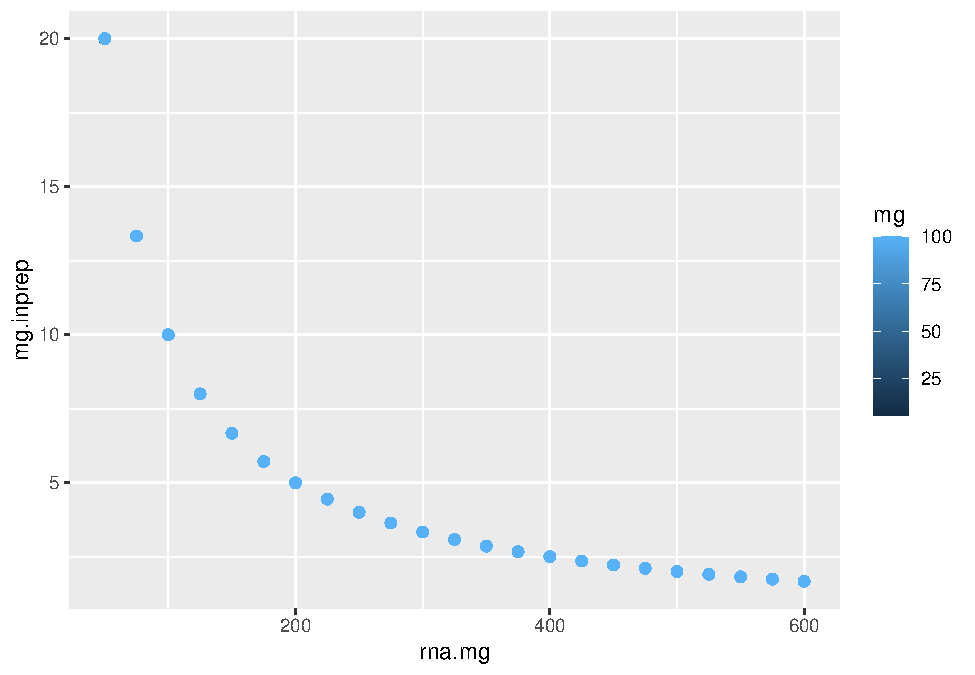
\includegraphics{thesis_files/figure-latex/unnamed-chunk-1-1.pdf}

\hypertarget{meta-analysis-of-within-session-training-volume}{%
\section{Meta-analysis of within-session training volume}\label{meta-analysis-of-within-session-training-volume}}

\hypertarget{literature-search-inclusion-criteria-and-coding-of-studies}{%
\subsection{Literature search, inclusion criteria and coding of studies}\label{literature-search-inclusion-criteria-and-coding-of-studies}}

A first set of studies were coded based previously published
meta-analyses {[}24,25{]}. For more recent studies, PubMed, Google
Scholar and SportDiscuss searches were made with search terms being
``training volume,'' ``resistance training,'' ``strength training,'' ``set,''
``muscle strength,'' ``muscle hypertrophy'' used in different combinations.
Studies examining the effect of within-session training volume on muscle
strength and mass, with all other training variables kept constant
between study groups were considered for inclusion in the meta-analysis.
Studies were further assessed for inclusion based on criteria being; (i)
participants described as healthy without medications affecting muscle
metabolism, (ii) interventions lasting at least 6 weeks and (iii) RT
performed without additional stimuli (e.g.~blood flow restriction) at
intensities above 65\% of 1RM or 20RM.

All available outcome measures of muscle mass and strength gains in
response to RT were extracted from each study with exception of outcomes
reported both as summaries and individual measures (e.g.~muscle
thickness reported as individual muscles and summarized for the whole
muscle group). In such cases the summary was used as outcome. Weekly
training volume was calculated as product of weekly sessions, number of
sets and exercises for each muscle group assessed for muscle hypertrophy
or strength gains. An intervention average of weekly sessions was used
when the number of sessions per week differed over the course of the
intervention. An exercise was assumed to influence an outcome when it
targeted prime movers also assessed for strength or muscle hypertrophy
measures. Participant characteristics were coded based on sex (male,
female or mixed when a study failed to discern between male and
females), age (young, middle-aged, old or mixed), body-mass index (BMI,
calculated from average body mass and height when BMI values were not
available), training status (trained, \textgreater{} 1 session per week during the
last 6 months leading up to the intervention; untrained \textless{} 1 session).
Study groups were considered independent also in studies utilizing
within-participant models.

\hypertarget{calculations-of-effect-sizes-and-statistical-analysis}{%
\subsection{Calculations of effect sizes and statistical analysis}\label{calculations-of-effect-sizes-and-statistical-analysis}}

Group-wise effect sizes were calculated for each outcome measure based
on the within-group change score pre- to post-training divided by the
pre-training standard deviation (SD). Pre-training SD's were calculated
as a pooled SD within outcome and study. Variances of the effect size
were calculated using an average effect size across all outcomes within
muscle strength or mass, and correlations specific to each measurement
type (isokinetic-, isometric- or repetition maximum strength tests;
muscle thickness, magnetic resonance imaging, dual energy X‐ray
absorptiometry) estimated from previous studies.\\
A correction factor () was applied to both effect sizes and their
variances.

Mixed-effects meta-regression models were used to model the effect of
weekly number of sets on RT-induced muscle mass and strength gains.
Models were fitted in a Bayesian framework using the brms-package
{[}256{]}.

\hypertarget{results-and-discussion}{%
\chapter{Results and Discussion}\label{results-and-discussion}}

\hypertarget{effects-of-different-training-volume-on-changes-in-muscle-size-and-function}{%
\section{Effects of different training volume on changes in muscle size and function}\label{effects-of-different-training-volume-on-changes-in-muscle-size-and-function}}

In Study I, the average increases in muscle strength and mass in each volume condition corresponded to what could be expected based on previous research in young, healthy participants (Table \ref{tab:csa-str-tab})
{[}257, 14{]},
indicating the general efficacy of the training program.




\begin{table}

\caption{\label{tab:csa-str-tab}Training induced changes in muscle CSA and average strength in Study I}
\centering
\fontsize{7}{9}\selectfont
\begin{tabular}[t]{lllll}
\toprule
 & Sex & Volume condition & Mean (SD) & Reference\\
\midrule
 &  & LOW & 3.05 (3.61) & \\
\cmidrule{3-4}
 & \multirow{-2}{*}{\raggedright\arraybackslash Female} & MOD & 5.02 (4.04) & \\
\cmidrule{2-4}
 &  & LOW & 3.83 (3.50) & \\
\cmidrule{3-4}
\multirow{-4}{*}{\raggedright\arraybackslash CSA \%-change} & \multirow{-2}{*}{\raggedright\arraybackslash Male} & MOD & 5.10 (3.71) & \multirow{-4}{*}{\raggedright\arraybackslash }\\
\cmidrule{1-5}
 &  & LOW & 0.04 (0.05) & \\
\cmidrule{3-4}
 & \multirow{-2}{*}{\raggedright\arraybackslash Female} & MOD & 0.07 (0.05) & \\
\cmidrule{2-4}
 &  & LOW & 0.05 (0.05) & \\
\cmidrule{3-4}
\multirow{-4}{*}{\raggedright\arraybackslash CSA \%-change per day} & \multirow{-2}{*}{\raggedright\arraybackslash Male} & MOD & 0.07 (0.05) & \multirow{-4}{*}{\raggedright\arraybackslash 0.11 [0.04-0.26]a}\\
\cmidrule{1-5}
 &  & LOW & 0.11 (0.13) & \\
\cmidrule{3-4}
 & \multirow{-2}{*}{\raggedright\arraybackslash Female} & MOD & 0.18 (0.15) & \multirow{-2}{*}{\raggedright\arraybackslash 0.08 (0.22)b}\\
\cmidrule{2-5}
 &  & LOW & 0.14 (0.12) & \\
\cmidrule{3-4}
\multirow{-4}{*}{\raggedright\arraybackslash CSA \%-change per session} & \multirow{-2}{*}{\raggedright\arraybackslash Male} & MOD & 0.19 (0.13) & \multirow{-2}{*}{\raggedright\arraybackslash 0.14 (0.14)b}\\
\cmidrule{1-5}
 &  & LOW & 21.0 (9.8) & \\
\cmidrule{3-4}
 & \multirow{-2}{*}{\raggedright\arraybackslash Female} & MOD & 27.8 (14.4) & \\
\cmidrule{2-4}
 &  & LOW & 19.2 (12.4) & \\
\cmidrule{3-4}
\multirow{-4}{*}{\raggedright\arraybackslash Average strength \%-change} & \multirow{-2}{*}{\raggedright\arraybackslash Male} & MOD & 23.1 (12.0) & \multirow{-4}{*}{\raggedright\arraybackslash }\\
\cmidrule{1-5}
 &  & LOW & 0.77 (0.36) & \\
\cmidrule{3-4}
 & \multirow{-2}{*}{\raggedright\arraybackslash Female} & MOD & 1.00 (0.49) & \multirow{-2}{*}{\raggedright\arraybackslash 0.67 (0.35)b}\\
\cmidrule{2-5}
 &  & LOW & 0.72 (0.48) & \\
\cmidrule{3-4}
\multirow{-4}{*}{\raggedright\arraybackslash Average strength \%-change per session} & \multirow{-2}{*}{\raggedright\arraybackslash Male} & MOD & 0.87 (0.46) & \multirow{-2}{*}{\raggedright\arraybackslash 0.47 (0.22)b}\\
\bottomrule
\multicolumn{5}{l}{\textsuperscript{a} Estimates from Wernbom et al. {[}257{]}}\\
\multicolumn{5}{l}{\textsuperscript{b} Estimates from Ahtiainen et al. {[}14{]}}\\
\end{tabular}
\end{table}
\begin{figure}

{\centering 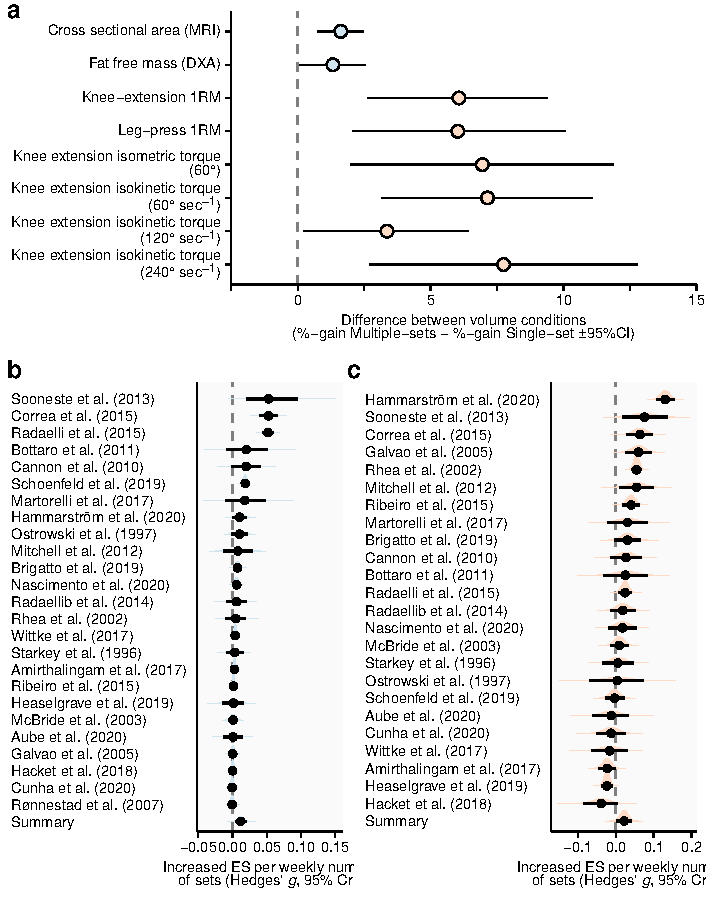
\includegraphics{thesis_files/figure-latex/comb-fig-s1-1} 

}

\caption[Differences in training induced changes to muscle mass and strength measures between volume conditions in Study I]{Differences in training induced relative changes in muscle mass and strength measures. Estimates are derived from ANCOVA models controling for baseline values.}\label{fig:comb-fig-s1}
\end{figure}
The multiple-sets (moderate-volume) condition consistently showed favorable adaptations when compared to the single-set (low-volume) condition in measures of muscle hypertrophy and strength gains (Figure \ref{fig:comb-fig-s1}).
In an attempt to explain differences in training outcomes between volume-conditions, selected molecular markers with known influence on adaptations to resistance training were investigated for volume-dependency.
First, acute activation of signaling along the mechanosensitive mTORC1-pathway has previously been shown to correlate with training-induced muscle growth
{[}157, 172, 258{]},
presumably trough increased translation indicated by greater ribosomal association with mRNA
{[}157{]}.
A commonly used readout of mTORC1-signaling is the phosphorylation of S6-kinase (S6K1) at Thr\textsuperscript{389}/Thr\textsuperscript{412} which in turn precedes phosphorylation of ribosomal protein S6 (rpS6, see Figure \ref{fig:mtor-fig}a).
In the present study, exercise-induced S6K1\textsuperscript{Thr\textsuperscript{389}/Thr\textsuperscript{412}} phosphorylation was indeed shown to be volume dependent along with phosphorylation of rpS6\textsuperscript{Ser\textsuperscript{235/236}} and mTOR\textsuperscript{Ser\textsuperscript{2448}} (Figure \ref{fig:mtor-fig} b).
It is recognized that phosphorylation of mTOR itself at Ser\textsuperscript{2448} primarily should be regarded as indicative for negative feedback as this site is phosphorylated due to S6K1 activity
{[}259{]} (Figure \ref{fig:mtor-fig} a).
It is also recognized that the phosphorylation status of rpS6 at Ser\textsuperscript{235/236} is not solely due to mTORC1 signalling as both mTORC1 and extracellular signal-regulated kinases (ERK)-signalling converges here
{[}260{]}.
Together these observations indicates larger perturbations along the mTORC1 signaling axis which confirms previous observations showing exercise-volume dependency of mTORC1 related signaling\\
{[}20, 21, 22{]}.
Interestingly, albeit with limited resolution, Terzis et al., did not find any clear volume dependency in exercise induced activation of either ERK 1/2 nor p38
{[}172{]}
suggesting that the relative contribution of different pathways to activation of downstream effectors may differ depending on mechanical stimuli.
It should however be noted that the present, and previous studies are limited in their temopral resolution and different patterns over time in different volume conditions cannot be ruled out.

The importance of mTORC1 signalling in protein synthesis in the acute phase after resistance exercise is well established.
In humans, administration of rapamycin, a selective inhibitor of mTORC1, prior to resistance exercise leads to delayed or blunted activation of mTORC1 effectors such as
S6K1\textsuperscript{Thr\textsuperscript{389}},
S6K1\textsuperscript{Thr\textsuperscript{421}/Ser\textsuperscript{424}},
rpS6\textsuperscript{Ser\textsuperscript{235/236}} and
rpS6\textsuperscript{Ser\textsuperscript{240/244}} as well as
unchanged levels of phopshorylation of 4E-BP1 and eEF2
concomitantly with abolished exercise-induced increase in protein synthesis
{[}173{]}.
Volume dependent increase in mTORC1 signalling also coincide with larger protein synthesis rates
{[}20{]}.
As such, volume dependence of mTORC1-related signalling suggests that higher within-session volume can be regarded as leading to an increased potential for protein synthesis in the acute-phase after exercise.
However, an increased signalling through this pathway could also be interpreted as indicative for increased ribosomal biogenesis.
\begin{figure}

{\centering 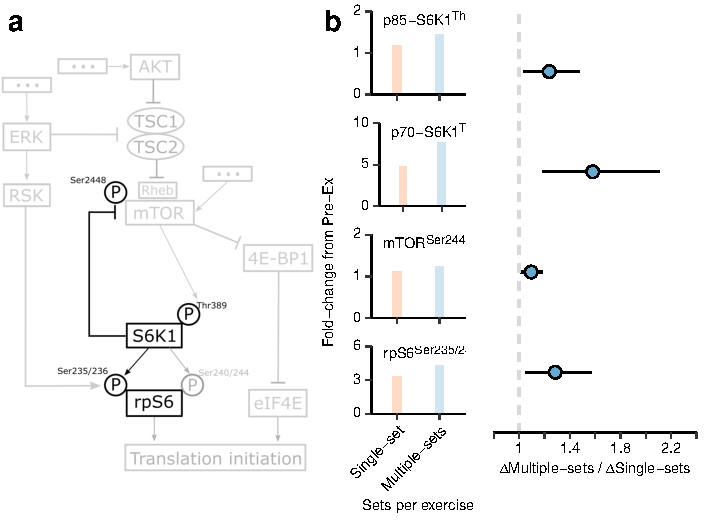
\includegraphics{thesis_files/figure-latex/mtor-fig-1} 

}

\caption[Differences between volume conditions in exercise induced phosphorylation of proteins related to mTORC1 signaling]{Measured phosphorylation sites in context (a) and differences between volume conditions in phosphorylation status of S6K1 at Thr \textsuperscript{389} (p70) Thr \textsuperscript{412} (p85), rpS6 at Ser \textsuperscript{235 236} and mTOR at Ser \textsuperscript{2448} induced by acute exercise and expressed as fold-changes (b). Estimates are derived from ANCOVA models controling for baseline values. Values in b are point estimates with 95\% confidence intervals.}\label{fig:mtor-fig}
\end{figure}
Indeed, mTORC1 affects ribosomal biogenesis through multiple mechanisms including activation of transcriptional programs related to ribosomal biogenesis (mediated through S6K1)
{[}187{]},
selective translation of specific mRNA related to ribosomal biogenesis
{[}188{]}
which in turn stimulates to increased ribosomal RNA transcription, mediated by cyclin D1 abundance and UBF availability
{[}189{]}.
\begin{figure}

{\centering 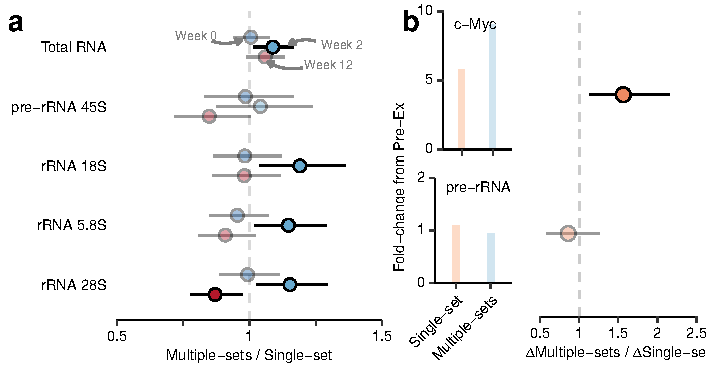
\includegraphics{thesis_files/figure-latex/rrna-fig-1} 

}

\caption[Differences between volume conditions total RNA and ribosomal RNA]{Differences between volume conditions in total RNA and ribosomal RNA-species (pre-rRNA 45S, rRNA 18S, rRNA 5.8S and rRNA 28S) measured at rest during the course of Study I (a). Acute changes in abundance of c-Myc mRNA and pre-rRNA 45S in response to acute exercise in Week 2 and differences between volume conditions (b). Errorbars represents 95\% confidence intervals, transparent points and errorbars signifies that the confidence interval contain 1.}\label{fig:rrna-fig}
\end{figure}
As ribosomal RNA is the most abundant constituent of muscle RNA it provides an estimate of muscle ribosomal abundance when expressed per unit tissue weight
{[}162, 164{]}.
From baseline to prior to the fifth training session (Week 2), total RNA per mg tissue increased by \(\sim\) 19 and 34\% in the single-set and multiple-sets condition, respectively. Total RNA levels were still elevated above baseline after the intervention (Week 12, single-set \(\sim\) 13; multiple-sets \(\sim\) 20\%). Similar patterns were seen in target analysis of ribosomal RNA using qPCR (single-set increase from baseline to Week 2 \(\sim\) 8-44\% and Week 12 \(\sim\) 14-36\%; multiple-sets \(\sim\) 31-57\% and Week 12 \(\sim\) 14-23\%). Comparing volume conditions revealed higher levels of total RNA and mature ribosomal RNA species in the multiple-sets condition at Week 2 (Figure \ref{fig:rrna-fig}a). At Week 12 differences between volume conditions were in total RNA less clear and ribosomal RNA 28S showing higher levels in the single-set leg (Figure \ref{fig:rrna-fig}a).

Together with indications of greater mTORC1 activation, analysis of c-Myc mRNA abundance in response to the fifth training session (Week 2) also showed volume-dependent regulation with exercise-induced increases being \textasciitilde{} 1.5-fold in response to the multiple-sets compared to the single-set condition (Figure \ref{fig:rrna-fig}b). c-Myc represents a rapamycin-insesitive signalling pathway known to also stimulating ribosomal biogenesis
{[}{]}
{[}{]}
\begin{table}

\caption{\label{tab:rna-csa-tab}Influence of RNA abundance on training-induced muscle growth measured with MRI}
\centering
\fontsize{8}{10}\selectfont
\begin{tabular}[t]{lrrrrll}
\toprule
\multicolumn{6}{c}{ } & \multicolumn{1}{c}{Standardized coefficients} \\
\cmidrule(l{3pt}r{3pt}){7-7}
 & Estimate & SE & df & \textit{t}-value & 95\% CI & Estimate [95\% CI]\\
\midrule
(Intercept) & -9.56 & 3.53 & 32 & -2.71 & [-16.75, -2.38] & 4.21 [3.02, 5.39]\\
\addlinespace[0.3em]
\multicolumn{7}{l}{\textbf{RNA abundance (ng mg\textsuperscript{-1})}}\\
\hspace{1em}Week 0 & 0.00 & 0.01 & 29 & 0.15 & [-0.016, 0.02] & 0.05 [-0.62, 0.72]\\
\hspace{1em}Week 2 & 0.02 & 0.01 & 29 & 4.26 & [0.012, 0.04] & 1.66 [0.86, 2.45]\\
\hspace{1em}Week 12 & 0.01 & 0.01 & 29 & 1.92 & [-0.001, 0.02] & 0.75 [-0.05, 1.54]\\
\bottomrule
\multicolumn{7}{l}{\textsuperscript{a} Standardized coefficients scaled by its SD}\\
\end{tabular}
\end{table}
\begin{figure}

{\centering 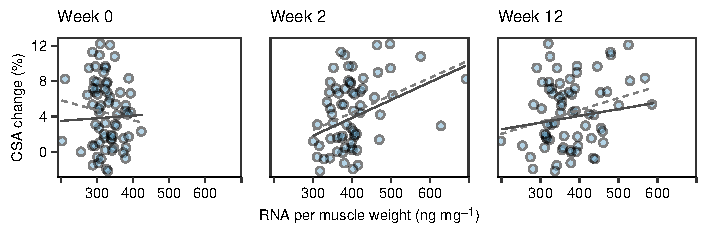
\includegraphics{thesis_files/figure-latex/rrna-csa-fig-1} 

}

\caption[Relationship between total RNA and training induced muscle growth]{Relationship between total RNA and training induced change in thigh cross sectional area (CSA) as measured by MRI. Dashed line represent 'naive' relationship, solid line represent adjusted reliationship as seen in \\ref{table:rna-csa-tab}.}\label{fig:rrna-csa-fig}
\end{figure}
Additionally, results from genetically modified mice lacking the mTORC1 effector S6K1 confirms its specific importance for maintenance of skeletal muscle size as these mice
{[}184{]}.
Particularly S6K1

mTORC controls protein synthesis trough multiple mechanisms
4E-BP1 and S6K1-rpS6

mTORC1 enhance translation of specific mRNA, including ribosoma biogenesis genes

{[}261{]}

{[}262{]}

Given these limitations in using mTORC-signalling as markers of muscle hypertrophy, it is not surprising that previous studies are ambiguous in their associative approach between acute mTORC1-related phosphorylation and hypertrophy in humans. Some studies find a strong correlation

{[}146, 263{]}.

{[}171{]};
{[}172{]};

This seems somewhat counterintuitive, as this pathway is a known regulator of translation initiation and elongation, as well as of ribosomal biogenesis
{[}189, 193,\\
187, 165{]}

Indeed, in the present study we observed volume-dependence of mTOR phosphorylation at Ser2448, which could be a sign of negative feedback from mTORC1-based activation of S6K1 {[}264{]}.
{[}24{]};
{[}23{]};
{[}25{]}{]}.
Furthermore, when a combining data from more recent studies indicates that a higher training volume is generally associated with increased muscle hypertrophy and strength gains (Figure \ref{fig:comb-fig-s1} and \ref{fig:comb-fig-s1}.

In Study II, training efficacy was assessed by comparing outcomes to a non-training control group. The training group displayed increases compared to the control group for both strength muscle thickness measures.

\hypertarget{acute-effects-of-diffrent-training-volume-on-determinants-of-muscle-protein-synthesis}{%
\section{Acute effects of diffrent training volume on determinants of muscle protein synthesis}\label{acute-effects-of-diffrent-training-volume-on-determinants-of-muscle-protein-synthesis}}

\hypertarget{general-discussion}{%
\chapter{General Discussion}\label{general-discussion}}

\hypertarget{conclusion}{%
\chapter*{Conclusion}\label{conclusion}}
\addcontentsline{toc}{chapter}{Conclusion}

If we don't want Conclusion to have a chapter number next to it, we can add the \texttt{\{-\}} attribute.

\textbf{More info}

And here's some other random info: the first paragraph after a chapter title or section head \emph{shouldn't be} indented, because indents are to tell the reader that you're starting a new paragraph. Since that's obvious after a chapter or section title, proper typesetting doesn't add an indent there.

\backmatter

\hypertarget{references}{%
\chapter*{References}\label{references}}
\addcontentsline{toc}{chapter}{References}

\markboth{References}{References}
\twocolumn

\setlength{\parskip}{4pt}

\rightskip3em

\footnotesize

\hypertarget{refs}{}
\begin{CSLReferences}{0}{0}
\leavevmode\hypertarget{ref-RN2512}{}%
\CSLLeftMargin{{[}1{]} }
\CSLRightInline{Li R, Xia J, Zhang XI, Gathirua-Mwangi WG, Guo J, Li Y, et al. Associations of muscle mass and strength with all-cause mortality among US older adults. Medicine and Science in Sports and Exercise 2018;50:458--67. \url{https://doi.org/10.1249/MSS.0000000000001448}.}

\leavevmode\hypertarget{ref-RN2808}{}%
\CSLLeftMargin{{[}2{]} }
\CSLRightInline{García-Hermoso A, Cavero-Redondo I, Ramírez-Vélez R, Ruiz JR, Ortega FB, Lee D-C, et al. Muscular strength as a predictor of all-cause mortality in an apparently healthy population: A systematic review and meta-analysis of data from approximately 2 million men and women. Archives of Physical Medicine and Rehabilitation 2018;99:2100--2113.e5. https://doi.org/\url{https://doi.org/10.1016/j.apmr.2018.01.008}.}

\leavevmode\hypertarget{ref-RN2513}{}%
\CSLLeftMargin{{[}3{]} }
\CSLRightInline{Fukasawa H, Kaneko M, Niwa H, Matsuyama T, Yasuda H, Kumagai H, et al. Lower thigh muscle mass is associated with all-cause and cardiovascular mortality in elderly hemodialysis patients. European Journal of Clinical Nutrition 2017;71:64--9. \url{https://doi.org/10.1038/ejcn.2016.186}.}

\leavevmode\hypertarget{ref-RN2514}{}%
\CSLLeftMargin{{[}4{]} }
\CSLRightInline{Miyake H, Kanazawa I, Tanaka KI, Sugimoto T. Low skeletal muscle mass is associated with the risk of all-cause mortality in patients with type 2 diabetes mellitus. Ther Adv Endocrinol Metab 2019;10:2042018819842971. \url{https://doi.org/10.1177/2042018819842971}.}

\leavevmode\hypertarget{ref-RN2809}{}%
\CSLLeftMargin{{[}5{]} }
\CSLRightInline{Ruiz JR, Sui X, Lobelo F, Morrow JR, Jackson AW, Sjöström M, et al. Association between muscular strength and mortality in men: Prospective cohort study. BMJ 2008;337:a439. \url{https://doi.org/10.1136/bmj.a439}.}

\leavevmode\hypertarget{ref-RN2515}{}%
\CSLLeftMargin{{[}6{]} }
\CSLRightInline{Szulc P, Munoz F, Marchand F, Chapurlat R, Delmas PD. Rapid loss of appendicular skeletal muscle mass is associated with higher all-cause mortality in older men: The prospective MINOS study. Am J Clin Nutr 2010;91:1227--36. \url{https://doi.org/10.3945/ajcn.2009.28256}.}

\leavevmode\hypertarget{ref-RN2516}{}%
\CSLLeftMargin{{[}7{]} }
\CSLRightInline{Abramowitz MK, Hall CB, Amodu A, Sharma D, Androga L, Hawkins M. Muscle mass, BMI, and mortality among adults in the united states: A population-based cohort study. PLoS One 2018;13:e0194697. \url{https://doi.org/10.1371/journal.pone.0194697}.}

\leavevmode\hypertarget{ref-RN2517}{}%
\CSLLeftMargin{{[}8{]} }
\CSLRightInline{Janssen I, Heymsfield SB, Ross R. Low relative skeletal muscle mass (sarcopenia) in older persons is associated with functional impairment and physical disability. J Am Geriatr Soc 2002;50:889--96. \url{https://doi.org/10.1046/j.1532-5415.2002.50216.x}.}

\leavevmode\hypertarget{ref-RN2532}{}%
\CSLLeftMargin{{[}9{]} }
\CSLRightInline{Sousa AS, Guerra RS, Fonseca I, Pichel F, Ferreira S, Amaral TF. Financial impact of sarcopenia on hospitalization costs. Eur J Clin Nutr 2016;70:1046--51. \url{https://doi.org/10.1038/ejcn.2016.73}.}

\leavevmode\hypertarget{ref-RN2184}{}%
\CSLLeftMargin{{[}10{]} }
\CSLRightInline{Pinedo-Villanueva R, Westbury LD, Syddall HE, Sanchez-Santos MT, Dennison EM, Robinson SM, et al. Health care costs associated with muscle weakness: A UK population-based estimate. Calcif Tissue Int 2019;104:137--44. \url{https://doi.org/10.1007/s00223-018-0478-1}.}

\leavevmode\hypertarget{ref-RN763}{}%
\CSLLeftMargin{{[}11{]} }
\CSLRightInline{Wolfe RR. The underappreciated role of muscle in health and disease. Am J Clin Nutr 2006;84:475--82.}

\leavevmode\hypertarget{ref-RN2526}{}%
\CSLLeftMargin{{[}12{]} }
\CSLRightInline{Arden NK, Spector TD. Genetic influences on muscle strength, lean body mass, and bone mineral density: A twin study. Journal of Bone and Mineral Research 1997;12:2076--81. \url{https://doi.org/10.1359/jbmr.1997.12.12.2076}.}

\leavevmode\hypertarget{ref-RN2527}{}%
\CSLLeftMargin{{[}13{]} }
\CSLRightInline{Roth SM. Genetic aspects of skeletal muscle strength and mass with relevance to sarcopenia. BoneKEy Reports 2012;1:58--8. \url{https://doi.org/10.1038/bonekey.2012.58}.}

\leavevmode\hypertarget{ref-RN1741}{}%
\CSLLeftMargin{{[}14{]} }
\CSLRightInline{Ahtiainen JP, Walker S, Peltonen H, Holviala J, Sillanpaa E, Karavirta L, et al. Heterogeneity in resistance training-induced muscle strength and mass responses in men and women of different ages. Age (Dordr) 2016;38:10. \url{https://doi.org/10.1007/s11357-015-9870-1}.}

\leavevmode\hypertarget{ref-RN2534}{}%
\CSLLeftMargin{{[}15{]} }
\CSLRightInline{Grgic J, Garofolini A, Orazem J, Sabol F, Schoenfeld BJ, Pedisic Z. Effects of resistance training on muscle size and strength in very elderly adults: A systematic review and meta-analysis of randomized controlled trials. Sports Med 2020. \url{https://doi.org/10.1007/s40279-020-01331-7}.}

\leavevmode\hypertarget{ref-RN2536}{}%
\CSLLeftMargin{{[}16{]} }
\CSLRightInline{Faigenbaum AD, Myer GD. Resistance training among young athletes: Safety, efficacy and injury prevention effects. British Journal of Sports Medicine 2010;44:56. \url{https://doi.org/10.1136/bjsm.2009.068098}.}

\leavevmode\hypertarget{ref-RN1}{}%
\CSLLeftMargin{{[}17{]} }
\CSLRightInline{Ratamess N, Alvar BA, Evetoch TK, Housh TJ, Kibler B, Kraemer WJ, et al. American college of sports medicine position stand. Progression models in resistance training for healthy adults. Med Sci Sports Exerc 2009;41:687--708. \url{https://doi.org/10.1249/MSS.0b013e3181915670}.}

\leavevmode\hypertarget{ref-RN798}{}%
\CSLLeftMargin{{[}18{]} }
\CSLRightInline{Bird SP, Tarpenning KM, Marino FE. Designing resistance training programmes to enhance muscular fitness: A review of the acute programme variables. Sports Med 2005;35:841--51.}

\leavevmode\hypertarget{ref-RN2538}{}%
\CSLLeftMargin{{[}19{]} }
\CSLRightInline{Feigenbaum MS, Pollock ML. Prescription of resistance training for health and disease. Med Sci Sports Exerc 1999;31:38--45. \url{https://doi.org/10.1097/00005768-199901000-00008}.}

\leavevmode\hypertarget{ref-RN791}{}%
\CSLLeftMargin{{[}20{]} }
\CSLRightInline{Burd NA, Holwerda AM, Selby KC, West DW, Staples AW, Cain NE, et al. Resistance exercise volume affects myofibrillar protein synthesis and anabolic signalling molecule phosphorylation in young men. J Physiol 2010;588:3119--30. \url{https://doi.org/10.1113/jphysiol.2010.192856}.}

\leavevmode\hypertarget{ref-RN784}{}%
\CSLLeftMargin{{[}21{]} }
\CSLRightInline{Terzis G, Spengos K, Mascher H, Georgiadis G, Manta P, Blomstrand E. The degree of p70 S6k and S6 phosphorylation in human skeletal muscle in response to resistance exercise depends on the training volume. Eur J Appl Physiol 2010;110:835--43. \url{https://doi.org/10.1007/s00421-010-1527-2}.}

\leavevmode\hypertarget{ref-RN1837}{}%
\CSLLeftMargin{{[}22{]} }
\CSLRightInline{Ahtiainen JP, Walker S, Silvennoinen M, Kyrolainen H, Nindl BC, Hakkinen K, et al. Exercise type and volume alter signaling pathways regulating skeletal muscle glucose uptake and protein synthesis. Eur J Appl Physiol 2015;115:1835--45. \url{https://doi.org/10.1007/s00421-015-3155-3}.}

\leavevmode\hypertarget{ref-RN793}{}%
\CSLLeftMargin{{[}23{]} }
\CSLRightInline{Krieger JW. Single versus multiple sets of resistance exercise: A meta-regression. J Strength Cond Res 2009;23:1890--901. \url{https://doi.org/10.1519/JSC.0b013e3181b370be}.}

\leavevmode\hypertarget{ref-RN789}{}%
\CSLLeftMargin{{[}24{]} }
\CSLRightInline{Krieger JW. Single vs. Multiple sets of resistance exercise for muscle hypertrophy: A meta-analysis. J Strength Cond Res 2010;24:1150--9. \url{https://doi.org/10.1519/JSC.0b013e3181d4d436}.}

\leavevmode\hypertarget{ref-RN1767}{}%
\CSLLeftMargin{{[}25{]} }
\CSLRightInline{Schoenfeld BJ, Ogborn D, Krieger JW. Dose-response relationship between weekly resistance training volume and increases in muscle mass: A systematic review and meta-analysis. J Sports Sci 2016:1--0. \url{https://doi.org/10.1080/02640414.2016.1210197}.}

\leavevmode\hypertarget{ref-RN2063}{}%
\CSLLeftMargin{{[}26{]} }
\CSLRightInline{Choi J, Lee M, Lee JK, Kang D, Choi JY. Correlates associated with participation in physical activity among adults: A systematic review of reviews and update. BMC Public Health 2017;17:356. \url{https://doi.org/10.1186/s12889-017-4255-2}.}

\leavevmode\hypertarget{ref-RN794}{}%
\CSLLeftMargin{{[}27{]} }
\CSLRightInline{Carpinelli RN, Otto RM. Strength training. Single versus multiple sets. Sports Med 1998;26:73--84.}

\leavevmode\hypertarget{ref-RN2547}{}%
\CSLLeftMargin{{[}28{]} }
\CSLRightInline{Pickering C, Kiely J. Do non-responders to exercise exist---and if so, what should we do about them? Sports Medicine 2019;49:1--7. \url{https://doi.org/10.1007/s40279-018-01041-1}.}

\leavevmode\hypertarget{ref-RN2640}{}%
\CSLLeftMargin{{[}29{]} }
\CSLRightInline{Tipton CM. The history of "exercise is medicine" in ancient civilizations. Adv Physiol Educ 2014;38:109--17. \url{https://doi.org/10.1152/advan.00136.2013}.}

\leavevmode\hypertarget{ref-RN2663}{}%
\CSLLeftMargin{{[}30{]} }
\CSLRightInline{Pfister G. Cultural confrontations: German turnen, swedish gymnastics and english sport--european diversity in physical activities from a historical perspective. Culture, Sport, Society 2003;6:61--91.}

\leavevmode\hypertarget{ref-RN2634}{}%
\CSLLeftMargin{{[}31{]} }
\CSLRightInline{Nicoll EA. Principles of exercise therapy. British Medical Journal 1943;1:747--50. \url{https://doi.org/10.1136/bmj.1.4302.747}.}

\leavevmode\hypertarget{ref-RN2633}{}%
\CSLLeftMargin{{[}32{]} }
\CSLRightInline{Delorme TL. RESTORATION OF MUSCLE POWER BY HEAVY-RESISTANCE EXERCISES. JBJS 1945;27.}

\leavevmode\hypertarget{ref-RN2639}{}%
\CSLLeftMargin{{[}33{]} }
\CSLRightInline{Todd JS, Shurley JP, Todd TC. Thomas l. DeLorme and the science of progressive resistance exercise. J Strength Cond Res 2012;26:2913--23. \url{https://doi.org/10.1519/JSC.0b013e31825adcb4}.}

\leavevmode\hypertarget{ref-RN2641}{}%
\CSLLeftMargin{{[}34{]} }
\CSLRightInline{Delorme TL, Watkins AL. Technics of progressive resistance exercise. Arch Phys Med Rehabil 1948;29:263--73.}

\leavevmode\hypertarget{ref-RN2646}{}%
\CSLLeftMargin{{[}35{]} }
\CSLRightInline{Delorme TL, West FE, Shriber WJ. INFLUENCE OF PROGRESSIVE-RESISTANCE EXERCISES ON KNEE FUNCTION FOLLOWING FEMORAL FRACTURES. JBJS 1950;32.}

\leavevmode\hypertarget{ref-RN2632}{}%
\CSLLeftMargin{{[}36{]} }
\CSLRightInline{Houtz SJ, Parrish AM, Hellebrandt FA. The influence of heavy resistance exercise on strength. Physical Therapy 1946;26:299--304. \url{https://doi.org/10.1093/ptj/26.6.299}.}

\leavevmode\hypertarget{ref-RN2644}{}%
\CSLLeftMargin{{[}37{]} }
\CSLRightInline{Chui E. The effect of systematic weight training on athletic power. Research Quarterly American Association for Health, Physical Education and Recreation 1950;21:188--94. \url{https://doi.org/10.1080/10671188.1950.10624849}.}

\leavevmode\hypertarget{ref-RN2642}{}%
\CSLLeftMargin{{[}38{]} }
\CSLRightInline{Capen EK. The effect of systematic weight training on power, strength, and endurance. Research Quarterly American Association for Health, Physical Education and Recreation 1950;21:83--93. \url{https://doi.org/10.1080/10671188.1950.10624835}.}

\leavevmode\hypertarget{ref-RN2645}{}%
\CSLLeftMargin{{[}39{]} }
\CSLRightInline{Hettinger T, Müller EA. Muskelleistung und muskeltraining. Arbeitsphysiologie 1953;15:111--26. \url{https://doi.org/10.1007/BF00934143}.}

\leavevmode\hypertarget{ref-RN1477}{}%
\CSLLeftMargin{{[}40{]} }
\CSLRightInline{Capen EK. Study of four programs of heavy resistance exercises for development of muscular strength. Research Quarterly American Association for Health, Physical Education and Recreation 1956;27:132--42. \url{https://doi.org/10.1080/10671188.1956.10612864}.}

\leavevmode\hypertarget{ref-RN1472}{}%
\CSLLeftMargin{{[}41{]} }
\CSLRightInline{Galvao DA, Taaffe DR. Resistance exercise dosage in older adults: Single- versus multiset effects on physical performance and body composition. J Am Geriatr Soc 2005;53:2090--7. \url{https://doi.org/10.1111/j.1532-5415.2005.00494.x}.}

\leavevmode\hypertarget{ref-RN2659}{}%
\CSLLeftMargin{{[}42{]} }
\CSLRightInline{Berger RA. COMPARISON OF THE EFFECT OF VARIOUS WEIGHT TRAINING LOADS ON STRENGTH. Res Q 1965;36:141--6.}

\leavevmode\hypertarget{ref-RN2658}{}%
\CSLLeftMargin{{[}43{]} }
\CSLRightInline{Berger RA, Hardage B. Effect of maximum loads for each of ten repetitions on strength improvement. Res Q 1967;38:715--8.}

\leavevmode\hypertarget{ref-RN2656}{}%
\CSLLeftMargin{{[}44{]} }
\CSLRightInline{O'Shea P. Effects of selected weight training programs on the development of strength and muscle hypertrophy. Res Q 1966;37:95--102.}

\leavevmode\hypertarget{ref-RN2537}{}%
\CSLLeftMargin{{[}45{]} }
\CSLRightInline{Fleck SJ, Kraemer WJ. Designing resistance training programs. Fourth edition. Champaign, IL: Human Kinetics; 2014.}

\leavevmode\hypertarget{ref-RN2655}{}%
\CSLLeftMargin{{[}46{]} }
\CSLRightInline{American college of sports medicine position statement on the recommended quantity and quality of exercise for developing and maintaining fitness in healthy adults. Med Sci Sports 1978;10:vii--x.}

\leavevmode\hypertarget{ref-RN2654}{}%
\CSLLeftMargin{{[}47{]} }
\CSLRightInline{American college of sports medicine position stand. The recommended quantity and quality of exercise for developing and maintaining cardiorespiratory and muscular fitness in healthy adults. Med Sci Sports Exerc 1990;22:265--74.}

\leavevmode\hypertarget{ref-RN2666}{}%
\CSLLeftMargin{{[}48{]} }
\CSLRightInline{Manley AF. Physical activity and health: A report of the surgeon general. Diane Publishing; 1996.}

\leavevmode\hypertarget{ref-RN2667}{}%
\CSLLeftMargin{{[}49{]} }
\CSLRightInline{Bull FC, Al-Ansari SS, Biddle S, Borodulin K, Buman MP, Cardon G, et al. World health organization 2020 guidelines on physical activity and sedentary behaviour. British Journal of Sports Medicine 2020;54:1451--62.}

\leavevmode\hypertarget{ref-RN2696}{}%
\CSLLeftMargin{{[}50{]} }
\CSLRightInline{n.d.;2021.}

\leavevmode\hypertarget{ref-RN2678}{}%
\CSLLeftMargin{{[}51{]} }
\CSLRightInline{Sanford JA, Nogiec CD, Lindholm ME, Adkins JN, Amar D, Dasari S, et al. Molecular transducers of physical activity consortium (MoTrPAC): Mapping the dynamic responses to exercise. Cell 2020;181:1464--74. https://doi.org/\url{https://doi.org/10.1016/j.cell.2020.06.004}.}

\leavevmode\hypertarget{ref-RN2677}{}%
\CSLLeftMargin{{[}52{]} }
\CSLRightInline{Sparks LM. Exercise training response heterogeneity: Physiological and molecular insights. Diabetologia 2017;60:2329--36. \url{https://doi.org/10.1007/s00125-017-4461-6}.}

\leavevmode\hypertarget{ref-RN764}{}%
\CSLLeftMargin{{[}53{]} }
\CSLRightInline{Hubal MJ, Gordish-Dressman H, Thompson PD, Price TB, Hoffman EP, Angelopoulos TJ, et al. Variability in muscle size and strength gain after unilateral resistance training. Med Sci Sports Exerc 2005;37:964--72.}

\leavevmode\hypertarget{ref-RN1263}{}%
\CSLLeftMargin{{[}54{]} }
\CSLRightInline{Pescatello LS, Devaney JM, Hubal MJ, Thompson PD, Hoffman EP. Highlights from the functional single nucleotide polymorphisms associated with human muscle size and strength or FAMuSS study. Biomed Res Int 2013;2013:643575. \url{https://doi.org/10.1155/2013/643575}.}

\leavevmode\hypertarget{ref-RN826}{}%
\CSLLeftMargin{{[}55{]} }
\CSLRightInline{Thalacker-Mercer A, Stec M, Cui X, Cross J, Windham S, Bamman M. Cluster analysis reveals differential transcript profiles associated with resistance training-induced human skeletal muscle hypertrophy. Physiol Genomics 2013;45:499--507. \url{https://doi.org/10.1152/physiolgenomics.00167.2012}.}

\leavevmode\hypertarget{ref-RN2684}{}%
\CSLLeftMargin{{[}56{]} }
\CSLRightInline{Stokes T, Timmons JA, Crossland H, Tripp TR, Murphy K, McGlory C, et al. Molecular transducers of human skeletal muscle remodeling under different loading states. Cell Rep 2020;32:107980. \url{https://doi.org/10.1016/j.celrep.2020.107980}.}

\leavevmode\hypertarget{ref-RN2698}{}%
\CSLLeftMargin{{[}57{]} }
\CSLRightInline{Roth SM. Perspective on the future use of genomics in exercise prescription. J Appl Physiol (1985) 2008;104:1243--5. \url{https://doi.org/10.1152/japplphysiol.01000.2007}.}

\leavevmode\hypertarget{ref-RN758}{}%
\CSLLeftMargin{{[}58{]} }
\CSLRightInline{Timmons JA. Variability in training-induced skeletal muscle adaptation. J Appl Physiol (1985) 2011;110:846--53. \url{https://doi.org/10.1152/japplphysiol.00934.2010}.}

\leavevmode\hypertarget{ref-RN2681}{}%
\CSLLeftMargin{{[}59{]} }
\CSLRightInline{Hautala AJ, Kiviniemi AM, Mäkikallio TH, Kinnunen H, Nissilä S, Huikuri HV, et al. Individual differences in the responses to endurance and resistance training. Eur J Appl Physiol 2006;96:535--42. \url{https://doi.org/10.1007/s00421-005-0116-2}.}

\leavevmode\hypertarget{ref-RN2699}{}%
\CSLLeftMargin{{[}60{]} }
\CSLRightInline{Montero D, Lundby C. Refuting the myth of non-response to exercise training: 'Non-responders' do respond to higher dose of training. J Physiol 2017;595:3377--87. \url{https://doi.org/10.1113/jp273480}.}

\leavevmode\hypertarget{ref-RN346}{}%
\CSLLeftMargin{{[}61{]} }
\CSLRightInline{Wernbom M, Augustsson J, Thomeé R. The influence of frequency, intensity, volume and mode of strength training on whole muscle cross-sectional area in humans. Sports Med 2007;37:225--64.}

\leavevmode\hypertarget{ref-RN1596}{}%
\CSLLeftMargin{{[}62{]} }
\CSLRightInline{DeFreitas JM, Beck TW, Stock MS, Dillon MA, Kasishke 2nd P. R. An examination of the time course of training-induced skeletal muscle hypertrophy. Eur J Appl Physiol 2011;111:2785--90. \url{https://doi.org/10.1007/s00421-011-1905-4}.}

\leavevmode\hypertarget{ref-RN2113}{}%
\CSLLeftMargin{{[}63{]} }
\CSLRightInline{Stock MS, Mota JA, DeFranco RN, Grue KA, Jacobo AU, Chung E, et al. The time course of short-term hypertrophy in the absence of eccentric muscle damage. Eur J Appl Physiol 2017;117:989--1004. \url{https://doi.org/10.1007/s00421-017-3587-z}.}

\leavevmode\hypertarget{ref-RN2736}{}%
\CSLLeftMargin{{[}64{]} }
\CSLRightInline{Narici MV, Roi GS, Landoni L, Minetti AE, Cerretelli P. Changes in force, cross-sectional area and neural activation during strength training and detraining of the human quadriceps. Eur J Appl Physiol Occup Physiol 1989;59:310--9. \url{https://doi.org/10.1007/bf02388334}.}

\leavevmode\hypertarget{ref-RN2739}{}%
\CSLLeftMargin{{[}65{]} }
\CSLRightInline{Welle S, Totterman S, Thornton C. Effect of age on muscle hypertrophy induced by resistance training. J Gerontol A Biol Sci Med Sci 1996;51:M270--5. \url{https://doi.org/10.1093/gerona/51a.6.m270}.}

\leavevmode\hypertarget{ref-RN767}{}%
\CSLLeftMargin{{[}66{]} }
\CSLRightInline{Folland JP, Williams AG. The adaptations to strength training : Morphological and neurological contributions to increased strength. Sports Med 2007;37:145--68.}

\leavevmode\hypertarget{ref-RN2740}{}%
\CSLLeftMargin{{[}67{]} }
\CSLRightInline{Roberts BM, Nuckols G, Krieger JW. Sex differences in resistance training: A systematic review and meta-analysis. J Strength Cond Res 2020;34:1448--60. \url{https://doi.org/10.1519/jsc.0000000000003521}.}

\leavevmode\hypertarget{ref-RN752}{}%
\CSLLeftMargin{{[}68{]} }
\CSLRightInline{Peterson MD, Sen A, Gordon PM. Influence of resistance exercise on lean body mass in aging adults: A meta-analysis. Med Sci Sports Exerc 2011;43:249--58. \url{https://doi.org/10.1249/MSS.0b013e3181eb6265}.}

\leavevmode\hypertarget{ref-RN2199}{}%
\CSLLeftMargin{{[}69{]} }
\CSLRightInline{Morton RW, Murphy KT, McKellar SR, Schoenfeld BJ, Henselmans M, Helms E, et al. A systematic review, meta-analysis and meta-regression of the effect of protein supplementation on resistance training-induced gains in muscle mass and strength in healthy adults. Br J Sports Med 2018;52:376--84. \url{https://doi.org/10.1136/bjsports-2017-097608}.}

\leavevmode\hypertarget{ref-RN2745}{}%
\CSLLeftMargin{{[}70{]} }
\CSLRightInline{Lixandrao ME, Ugrinowitsch C, Berton R, Vechin FC, Conceicao MS, Damas F, et al. Magnitude of muscle strength and mass adaptations between high-load resistance training versus low-load resistance training associated with blood-flow restriction: A systematic review and meta-analysis. Sports Med 2018;48:361--78. \url{https://doi.org/10.1007/s40279-017-0795-y}.}

\leavevmode\hypertarget{ref-RN2741}{}%
\CSLLeftMargin{{[}71{]} }
\CSLRightInline{Murach KA, Dungan CM, Peterson CA, McCarthy JJ. Muscle fiber splitting is a physiological response to extreme loading in animals. Exerc Sport Sci Rev 2019;47:108--15. \url{https://doi.org/10.1249/jes.0000000000000181}.}

\leavevmode\hypertarget{ref-RN2742}{}%
\CSLLeftMargin{{[}72{]} }
\CSLRightInline{Sjöström M, Lexell J, Eriksson A, Taylor CC. Evidence of fibre hyperplasia in human skeletal muscles from healthy young men? A left-right comparison of the fibre number in whole anterior tibialis muscles. Eur J Appl Physiol Occup Physiol 1991;62:301--4. \url{https://doi.org/10.1007/bf00634963}.}

\leavevmode\hypertarget{ref-RN2754}{}%
\CSLLeftMargin{{[}73{]} }
\CSLRightInline{MacDougall JD, Sale DG, Alway SE, Sutton JR. Muscle fiber number in biceps brachii in bodybuilders and control subjects. J Appl Physiol Respir Environ Exerc Physiol 1984;57:1399--403. \url{https://doi.org/10.1152/jappl.1984.57.5.1399}.}

\leavevmode\hypertarget{ref-RN2731}{}%
\CSLLeftMargin{{[}74{]} }
\CSLRightInline{Lüthi JM, Howald H, Claassen H, Rösler K, Vock P, Hoppeler H. Structural changes in skeletal muscle tissue with heavy-resistance exercise. Int J Sports Med 1986;7:123--7. \url{https://doi.org/10.1055/s-2008-1025748}.}

\leavevmode\hypertarget{ref-RN2756}{}%
\CSLLeftMargin{{[}75{]} }
\CSLRightInline{Sweeney HL, Hammers DW. Muscle contraction. Cold Spring Harb Perspect Biol 2018;10. \url{https://doi.org/10.1101/cshperspect.a023200}.}

\leavevmode\hypertarget{ref-RN2669}{}%
\CSLLeftMargin{{[}76{]} }
\CSLRightInline{Straight CR, Fedewa MV, Toth MJ, Miller MS. Improvements in skeletal muscle fiber size with resistance training are age-dependent in older adults: A systematic review and meta-analysis. Journal of Applied Physiology 2020;129:392--403. \url{https://doi.org/10.1152/japplphysiol.00170.2020}.}

\leavevmode\hypertarget{ref-RN2758}{}%
\CSLLeftMargin{{[}77{]} }
\CSLRightInline{Bamman MM, Newcomer BR, Larson-Meyer DE, Weinsier RL, Hunter GR. Evaluation of the strength-size relationship in vivo using various muscle size indices. Med Sci Sports Exerc 2000;32:1307--13. \url{https://doi.org/10.1097/00005768-200007000-00019}.}

\leavevmode\hypertarget{ref-RN1142}{}%
\CSLLeftMargin{{[}78{]} }
\CSLRightInline{Erskine RM, Fletcher G, Folland JP. The contribution of muscle hypertrophy to strength changes following resistance training. Eur J Appl Physiol 2014. \url{https://doi.org/10.1007/s00421-014-2855-4}.}

\leavevmode\hypertarget{ref-RN2629}{}%
\CSLLeftMargin{{[}79{]} }
\CSLRightInline{Ikai M, Fukunaga T. A study on training effect on strength per unit cross-sectional area of muscle by means of ultrasonic measurement. Int Z Angew Physiol 1970;28:173--80. \url{https://doi.org/10.1007/bf00696025}.}

\leavevmode\hypertarget{ref-RN2737}{}%
\CSLLeftMargin{{[}80{]} }
\CSLRightInline{Young A, Stokes M, Round JM, Edwards RH. The effect of high-resistance training on the strength and cross-sectional area of the human quadriceps. Eur J Clin Invest 1983;13:411--7. \url{https://doi.org/10.1111/j.1365-2362.1983.tb00122.x}.}

\leavevmode\hypertarget{ref-RN2735}{}%
\CSLLeftMargin{{[}81{]} }
\CSLRightInline{Narici MV, Hoppeler H, Kayser B, Landoni L, Claassen H, Gavardi C, et al. Human quadriceps cross-sectional area, torque and neural activation during 6 months strength training. Acta Physiol Scand 1996;157:175--86. \url{https://doi.org/10.1046/j.1365-201X.1996.483230000.x}.}

\leavevmode\hypertarget{ref-RN2158}{}%
\CSLLeftMargin{{[}82{]} }
\CSLRightInline{Vigotsky AD, Schoenfeld BJ, Than C, Brown JM. Methods matter: The relationship between strength and hypertrophy depends on methods of measurement and analysis. PeerJ 2018;6:e5071. \url{https://doi.org/10.7717/peerj.5071}.}

\leavevmode\hypertarget{ref-RN2760}{}%
\CSLLeftMargin{{[}83{]} }
\CSLRightInline{Mattocks KT, Buckner SL, Jessee MB, Dankel SJ, Mouser JG, Loenneke JP. Practicing the test produces strength equivalent to higher volume training. Med Sci Sports Exerc 2017;49:1945--54. \url{https://doi.org/10.1249/mss.0000000000001300}.}

\leavevmode\hypertarget{ref-RN2219}{}%
\CSLLeftMargin{{[}84{]} }
\CSLRightInline{Carroll TJ, Herbert RD, Munn J, Lee M, Gandevia SC. Contralateral effects of unilateral strength training: Evidence and possible mechanisms. J Appl Physiol (1985) 2006;101:1514--22. \url{https://doi.org/10.1152/japplphysiol.00531.2006}.}

\leavevmode\hypertarget{ref-RN2766}{}%
\CSLLeftMargin{{[}85{]} }
\CSLRightInline{Green LA, Gabriel DA. The cross education of strength and skill following unilateral strength training in the upper and lower limbs. J Neurophysiol 2018;120:468--79. \url{https://doi.org/10.1152/jn.00116.2018}.}

\leavevmode\hypertarget{ref-RN2767}{}%
\CSLLeftMargin{{[}86{]} }
\CSLRightInline{Zijdewind I, Toering ST, Bessem B, Van Der Laan O, Diercks RL. Effects of imagery motor training on torque production of ankle plantar flexor muscles. Muscle Nerve 2003;28:168--73. \url{https://doi.org/10.1002/mus.10406}.}

\leavevmode\hypertarget{ref-RN2763}{}%
\CSLLeftMargin{{[}87{]} }
\CSLRightInline{Del Vecchio A, Casolo A, Negro F, Scorcelletti M, Bazzucchi I, Enoka R, et al. The increase in muscle force after 4~weeks of strength training is mediated by adaptations in motor unit recruitment and rate coding. J Physiol 2019;597:1873--87. \url{https://doi.org/10.1113/jp277250}.}

\leavevmode\hypertarget{ref-RN2764}{}%
\CSLLeftMargin{{[}88{]} }
\CSLRightInline{Gardiner P, Dai Y, Heckman CJ. Effects of exercise training on alpha-motoneurons. J Appl Physiol (1985) 2006;101:1228--36. \url{https://doi.org/10.1152/japplphysiol.00482.2006}.}

\leavevmode\hypertarget{ref-RN819}{}%
\CSLLeftMargin{{[}89{]} }
\CSLRightInline{Schiaffino S, Reggiani C. Fiber types in mammalian skeletal muscles. Physiol Rev 2011;91:1447--531. \url{https://doi.org/10.1152/physrev.00031.2010}.}

\leavevmode\hypertarget{ref-RN846}{}%
\CSLLeftMargin{{[}90{]} }
\CSLRightInline{Harridge SD, Bottinelli R, Canepari M, Pellegrino MA, Reggiani C, Esbjornsson M, et al. Whole-muscle and single-fibre contractile properties and myosin heavy chain isoforms in humans. Pflugers Arch 1996;432:913--20.}

\leavevmode\hypertarget{ref-RN2169}{}%
\CSLLeftMargin{{[}91{]} }
\CSLRightInline{Widrick JJ, Stelzer JE, Shoepe TC, Garner DP. Functional properties of human muscle fibers after short-term resistance exercise training. Am J Physiol Regul Integr Comp Physiol 2002;283:R408--16. \url{https://doi.org/10.1152/ajpregu.00120.2002}.}

\leavevmode\hypertarget{ref-RN849}{}%
\CSLLeftMargin{{[}92{]} }
\CSLRightInline{Lionikas A, Li M, Larsson L. Human skeletal muscle myosin function at physiological and non-physiological temperatures. Acta Physiol (Oxf) 2006;186:151--8. \url{https://doi.org/10.1111/j.1748-1716.2005.01516.x}.}

\leavevmode\hypertarget{ref-RN1885}{}%
\CSLLeftMargin{{[}93{]} }
\CSLRightInline{Essen B, Jansson E, Henriksson J, Taylor AW, Saltin B. Metabolic characteristics of fibre types in human skeletal muscle. Acta Physiol Scand 1975;95:153--65. \url{https://doi.org/10.1111/j.1748-1716.1975.tb10038.x}.}

\leavevmode\hypertarget{ref-RN2801}{}%
\CSLLeftMargin{{[}94{]} }
\CSLRightInline{Karatzaferi C, Haan A de, Mechelen W van, Sargeant AJ. Metabolism changes in single human fibres during brief maximal exercise. Exp Physiol 2001;86:411--5. \url{https://doi.org/10.1113/eph8602223}.}

\leavevmode\hypertarget{ref-RN2798}{}%
\CSLLeftMargin{{[}95{]} }
\CSLRightInline{Simoneau JA, Bouchard C. Genetic determinism of fiber type proportion in human skeletal muscle. Faseb j 1995;9:1091--5. \url{https://doi.org/10.1096/fasebj.9.11.7649409}.}

\leavevmode\hypertarget{ref-RN2795}{}%
\CSLLeftMargin{{[}96{]} }
\CSLRightInline{Simoneau JA, Bouchard C. Human variation in skeletal muscle fiber-type proportion and enzyme activities. Am J Physiol 1989;257:E567--72. \url{https://doi.org/10.1152/ajpendo.1989.257.4.E567}.}

\leavevmode\hypertarget{ref-RN285}{}%
\CSLLeftMargin{{[}97{]} }
\CSLRightInline{Staron RS, Hagerman FC, Hikida RS, Murray TF, Hostler DP, Crill MT, et al. Fiber type composition of the vastus lateralis muscle of young men and women. J Histochem Cytochem 2000;48:623--9.}

\leavevmode\hypertarget{ref-RN2220}{}%
\CSLLeftMargin{{[}98{]} }
\CSLRightInline{Adams GR, Hather BM, Baldwin KM, Dudley GA. Skeletal muscle myosin heavy chain composition and resistance training. J Appl Physiol (1985) 1993;74:911--5. \url{https://doi.org/10.1152/jappl.1993.74.2.911}.}

\leavevmode\hypertarget{ref-RN2799}{}%
\CSLLeftMargin{{[}99{]} }
\CSLRightInline{Williamson DL, Gallagher PM, Carroll CC, Raue U, Trappe SW. Reduction in hybrid single muscle fiber proportions with resistance training in humans. J Appl Physiol (1985) 2001;91:1955--61. \url{https://doi.org/10.1152/jappl.2001.91.5.1955}.}

\leavevmode\hypertarget{ref-RN2056}{}%
\CSLLeftMargin{{[}100{]} }
\CSLRightInline{Andersen JL, Gruschy-Knudsen T. Rapid switch-off of the human myosin heavy chain IIX gene after heavy load muscle contractions is sustained for at least four days. Scand J Med Sci Sports 2018;28:371--80. \url{https://doi.org/10.1111/sms.12914}.}

\leavevmode\hypertarget{ref-RN1489}{}%
\CSLLeftMargin{{[}101{]} }
\CSLRightInline{Ellefsen S, Vikmoen O, Zacharoff E, Rauk I, Slettalokken G, Hammarstrom D, et al. Reliable determination of training-induced alterations in muscle fiber composition in human skeletal muscle using quantitative polymerase chain reaction. Scand J Med Sci Sports 2014;24:e332--42. \url{https://doi.org/10.1111/sms.12185}.}

\leavevmode\hypertarget{ref-RN2057}{}%
\CSLLeftMargin{{[}102{]} }
\CSLRightInline{Andersen JL, Aagaard P. Myosin heavy chain IIX overshoot in human skeletal muscle. Muscle Nerve 2000;23:1095--104.}

\leavevmode\hypertarget{ref-RN2108}{}%
\CSLLeftMargin{{[}103{]} }
\CSLRightInline{Borina E, Pellegrino MA, D'Antona G, Bottinelli R. Myosin and actin content of human skeletal muscle fibers following 35 days bed rest. Scand J Med Sci Sports 2010;20:65--73. \url{https://doi.org/10.1111/j.1600-0838.2009.01029.x}.}

\leavevmode\hypertarget{ref-RN1505}{}%
\CSLLeftMargin{{[}104{]} }
\CSLRightInline{Burd NA, Andrews RJ, West DW, Little JP, Cochran AJ, Hector AJ, et al. Muscle time under tension during resistance exercise stimulates differential muscle protein sub-fractional synthetic responses in men. J Physiol 2012;590:351--62. \url{https://doi.org/10.1113/jphysiol.2011.221200}.}

\leavevmode\hypertarget{ref-RN2608}{}%
\CSLLeftMargin{{[}105{]} }
\CSLRightInline{Porter C, Reidy PT, Bhattarai N, Sidossis LS, Rasmussen BB. Resistance exercise training alters mitochondrial function in human skeletal muscle. Medicine and Science in Sports and Exercise 2015;47:1922--31. \url{https://doi.org/10.1249/MSS.0000000000000605}.}

\leavevmode\hypertarget{ref-RN2817}{}%
\CSLLeftMargin{{[}106{]} }
\CSLRightInline{Chan DC. Mitochondrial fusion and fission in mammals. Annu Rev Cell Dev Biol 2006;22:79--99. \url{https://doi.org/10.1146/annurev.cellbio.22.010305.104638}.}

\leavevmode\hypertarget{ref-RN2816}{}%
\CSLLeftMargin{{[}107{]} }
\CSLRightInline{Mishra P, Varuzhanyan G, Pham AH, Chan DC. Mitochondrial dynamics is a distinguishing feature of skeletal muscle fiber types and regulates organellar compartmentalization. Cell Metab 2015;22:1033--44. \url{https://doi.org/10.1016/j.cmet.2015.09.027}.}

\leavevmode\hypertarget{ref-RN2818}{}%
\CSLLeftMargin{{[}108{]} }
\CSLRightInline{Lin J, Wu H, Tarr PT, Zhang CY, Wu Z, Boss O, et al. Transcriptional co-activator PGC-1 alpha drives the formation of slow-twitch muscle fibres. Nature 2002;418:797--801. \url{https://doi.org/10.1038/nature00904}.}

\leavevmode\hypertarget{ref-RN2819}{}%
\CSLLeftMargin{{[}109{]} }
\CSLRightInline{Handschin C, Chin S, Li P, Liu F, Maratos-Flier E, Lebrasseur NK, et al. Skeletal muscle fiber-type switching, exercise intolerance, and myopathy in PGC-1alpha muscle-specific knock-out animals. J Biol Chem 2007;282:30014--21. \url{https://doi.org/10.1074/jbc.M704817200}.}

\leavevmode\hypertarget{ref-RN2775}{}%
\CSLLeftMargin{{[}110{]} }
\CSLRightInline{Greendale GA, Huang MH, Wang Y, Finkelstein JS, Danielson ME, Sternfeld B. Sport and home physical activity are independently associated with bone density. Med Sci Sports Exerc 2003;35:506--12. \url{https://doi.org/10.1249/01.Mss.0000056725.64347.C9}.}

\leavevmode\hypertarget{ref-RN2771}{}%
\CSLLeftMargin{{[}111{]} }
\CSLRightInline{Magnusson SP, Narici MV, Maganaris CN, Kjaer M. Human tendon behaviour and adaptation, in vivo. J Physiol 2008;586:71--81. \url{https://doi.org/10.1113/jphysiol.2007.139105}.}

\leavevmode\hypertarget{ref-RN2774}{}%
\CSLLeftMargin{{[}112{]} }
\CSLRightInline{Miller LE, Nickols-Richardson SM, Wootten DF, Ramp WK, Steele CR, Cotton JR, et al. Isokinetic resistance training increases tibial bending stiffness in young women. Calcif Tissue Int 2009;84:446--52. \url{https://doi.org/10.1007/s00223-009-9247-5}.}

\leavevmode\hypertarget{ref-RN2772}{}%
\CSLLeftMargin{{[}113{]} }
\CSLRightInline{Massey GJ, Balshaw TG, Maden-Wilkinson TM, Folland JP. Tendinous tissue properties after short- and long-term functional overload: Differences between controls, 12~weeks and 4~years of resistance training. Acta Physiol (Oxf) 2018;222:e13019. \url{https://doi.org/10.1111/apha.13019}.}

\leavevmode\hypertarget{ref-RN2770}{}%
\CSLLeftMargin{{[}114{]} }
\CSLRightInline{Kjaer M, Magnusson P, Krogsgaard M, Boysen Møller J, Olesen J, Heinemeier K, et al. Extracellular matrix adaptation of tendon and skeletal muscle to exercise. J Anat 2006;208:445--50. \url{https://doi.org/10.1111/j.1469-7580.2006.00549.x}.}

\leavevmode\hypertarget{ref-RN2783}{}%
\CSLLeftMargin{{[}115{]} }
\CSLRightInline{Borg TK, Caulfield JB. Morphology of connective tissue in skeletal muscle. Tissue Cell 1980;12:197--207. \url{https://doi.org/10.1016/0040-8166(80)90061-0}.}

\leavevmode\hypertarget{ref-RN2421}{}%
\CSLLeftMargin{{[}116{]} }
\CSLRightInline{Kjaer M. Role of extracellular matrix in adaptation of tendon and skeletal muscle to mechanical loading. Physiol Rev 2004;84:649--98. \url{https://doi.org/10.1152/physrev.00031.2003}.}

\leavevmode\hypertarget{ref-RN2788}{}%
\CSLLeftMargin{{[}117{]} }
\CSLRightInline{Miller BF, Olesen JL, Hansen M, Døssing S, Crameri RM, Welling RJ, et al. Coordinated collagen and muscle protein synthesis in human patella tendon and quadriceps muscle after exercise. J Physiol 2005;567:1021--33. \url{https://doi.org/10.1113/jphysiol.2005.093690}.}

\leavevmode\hypertarget{ref-RN2454}{}%
\CSLLeftMargin{{[}118{]} }
\CSLRightInline{Holm L, Hall G van, Rose AJ, Miller BF, Doessing S, Richter EA, et al. Contraction intensity and feeding affect collagen and myofibrillar protein synthesis rates differently in human skeletal muscle. Am J Physiol Endocrinol Metab 2010;298:E257--69. \url{https://doi.org/10.1152/ajpendo.00609.2009}.}

\leavevmode\hypertarget{ref-RN2298}{}%
\CSLLeftMargin{{[}119{]} }
\CSLRightInline{Damas F, Ugrinowitsch C, Libardi CA, Jannig PR, Hector AJ, McGlory C, et al. Resistance training in young men induces muscle transcriptome-wide changes associated with muscle structure and metabolism refining the response to exercise-induced stress. Eur J Appl Physiol 2018;118:2607--16. \url{https://doi.org/10.1007/s00421-018-3984-y}.}

\leavevmode\hypertarget{ref-RN774}{}%
\CSLLeftMargin{{[}120{]} }
\CSLRightInline{Raue U, Trappe TA, Estrem ST, Qian HR, Helvering LM, Smith RC, et al. Transcriptome signature of resistance exercise adaptations: Mixed muscle and fiber type specific profiles in young and old adults. J Appl Physiol (1985) 2012;112:1625--36. \url{https://doi.org/10.1152/japplphysiol.00435.2011}.}

\leavevmode\hypertarget{ref-RN2457}{}%
\CSLLeftMargin{{[}121{]} }
\CSLRightInline{Moore DR, Phillips SM, Babraj JA, Smith K, Rennie MJ. Myofibrillar and collagen protein synthesis in human skeletal muscle in young men after maximal shortening and lengthening contractions. Am J Physiol Endocrinol Metab 2005;288:E1153--9. \url{https://doi.org/10.1152/ajpendo.00387.2004}.}

\leavevmode\hypertarget{ref-RN1504}{}%
\CSLLeftMargin{{[}122{]} }
\CSLRightInline{Erskine RM, Jones DA, Maffulli N, Williams AG, Stewart CE, Degens H. What causes in vivo muscle specific tension to increase following resistance training? Exp Physiol 2011;96:145--55. \url{https://doi.org/10.1113/expphysiol.2010.053975}.}

\leavevmode\hypertarget{ref-RN2575}{}%
\CSLLeftMargin{{[}123{]} }
\CSLRightInline{Evans JW. Periodized resistance training for enhancing skeletal muscle hypertrophy and strength: A mini-review. Frontiers in Physiology 2019;10:13--3. \url{https://doi.org/10.3389/fphys.2019.00013}.}

\leavevmode\hypertarget{ref-RN2572}{}%
\CSLLeftMargin{{[}124{]} }
\CSLRightInline{Grgic J, Mikulic P, Podnar H, Pedisic Z. Effects of linear and daily undulating periodized resistance training programs on measures of muscle hypertrophy: A systematic review and meta-analysis. PeerJ 2017;5:e3695--5. \url{https://doi.org/10.7717/peerj.3695}.}

\leavevmode\hypertarget{ref-RN2571}{}%
\CSLLeftMargin{{[}125{]} }
\CSLRightInline{Schoenfeld BJ, Ogborn D, Krieger JW. Effects of resistance training frequency on measures of muscle hypertrophy: A systematic review and meta-analysis. Sports Med 2016;46:1689--97. \url{https://doi.org/10.1007/s40279-016-0543-8}.}

\leavevmode\hypertarget{ref-RN2569}{}%
\CSLLeftMargin{{[}126{]} }
\CSLRightInline{Schoenfeld BJ, Grgic J, Ogborn D, Krieger JW. Strength and hypertrophy adaptations between low- vs. High-load resistance training: A systematic review and meta-analysis. J Strength Cond Res 2017;31:3508--23. \url{https://doi.org/10.1519/jsc.0000000000002200}.}

\leavevmode\hypertarget{ref-RN1612}{}%
\CSLLeftMargin{{[}127{]} }
\CSLRightInline{Schoenfeld BJ, Ratamess NA, Peterson MD, Contreras B, Sonmez GT, Alvar BA. Effects of different volume-equated resistance training loading strategies on muscular adaptations in well-trained men. J Strength Cond Res 2014;28:2909--18. \url{https://doi.org/10.1519/JSC.0000000000000480}.}

\leavevmode\hypertarget{ref-RN2570}{}%
\CSLLeftMargin{{[}128{]} }
\CSLRightInline{Grgic J, Schoenfeld BJ, Davies TB, Lazinica B, Krieger JW, Pedisic Z. Effect of resistance training frequency on gains in muscular strength: A systematic review and meta-analysis. Sports Med 2018;48:1207--20. \url{https://doi.org/10.1007/s40279-018-0872-x}.}

\leavevmode\hypertarget{ref-RN2591}{}%
\CSLLeftMargin{{[}129{]} }
\CSLRightInline{Nunes JP, Grgic J, Cunha PM, Ribeiro AS, Schoenfeld BJ, Salles BF de, et al. What influence does resistance exercise order have on muscular strength gains and muscle hypertrophy? A systematic review and meta-analysis. Eur J Sport Sci 2020:1--9. \url{https://doi.org/10.1080/17461391.2020.1733672}.}

\leavevmode\hypertarget{ref-RN2492}{}%
\CSLLeftMargin{{[}130{]} }
\CSLRightInline{Ralston GW, Kilgore L, Wyatt FB, Baker JS. The effect of weekly set volume on strength gain: A meta-analysis. Sports Med 2017;47:2585--601. \url{https://doi.org/10.1007/s40279-017-0762-7}.}

\leavevmode\hypertarget{ref-RN2130}{}%
\CSLLeftMargin{{[}131{]} }
\CSLRightInline{Baz-Valle E, Fontes-Villalba M, Santos-Concejero J. Total number of sets as a training volume quantification method for muscle hypertrophy: A systematic review. J Strength Cond Res 2018. \url{https://doi.org/10.1519/jsc.0000000000002776}.}

\leavevmode\hypertarget{ref-RN1476}{}%
\CSLLeftMargin{{[}132{]} }
\CSLRightInline{Berger R. Effect of varied weight training programs on strength. Research Quarterly American Association for Health, Physical Education and Recreation 1962;33:168--81. \url{https://doi.org/10.1080/10671188.1962.10613188}.}

\leavevmode\hypertarget{ref-RN2568}{}%
\CSLLeftMargin{{[}133{]} }
\CSLRightInline{Junyoung H, Corinna NR, John DS, Sukho L. Low volume progressive single set of resistance training is as effective as high volume multiple sets of resistance protocol on muscle strength and power. International Journal of Applied Sports Sciences : IJASS 2015;27:33--42. \url{https://doi.org/10.24985/ijass.2015.27.1.33}.}

\leavevmode\hypertarget{ref-RN2201}{}%
\CSLLeftMargin{{[}134{]} }
\CSLRightInline{Carpinelli RN. Science versus opinion. British Journal of Sports Medicine 2004;38:240--2. \url{https://doi.org/10.1136/bjsm.2003.010710}.}

\leavevmode\hypertarget{ref-RN2465}{}%
\CSLLeftMargin{{[}135{]} }
\CSLRightInline{Ribeiro AS, Schoenfeld BJ, Pina FLC, Souza MF, Nascimento MA, Santos L dos, et al. Resistance training in older women: Comparison of single vs. Multiple sets on muscle strength and body composition. Isokinetics and Exercise Science 2015;23:53--60. \url{https://doi.org/10.3233/IES-140564}.}

\leavevmode\hypertarget{ref-RN2464}{}%
\CSLLeftMargin{{[}136{]} }
\CSLRightInline{Correa CS, Teixeira BC, Cobos RC, Macedo RC, Kruger RL, Carteri RB, et al. High-volume resistance training reduces postprandial lipaemia in postmenopausal women. J Sports Sci 2015;33:1890--901. \url{https://doi.org/10.1080/02640414.2015.1017732}.}

\leavevmode\hypertarget{ref-RN2463}{}%
\CSLLeftMargin{{[}137{]} }
\CSLRightInline{Bottaro M, Veloso J, Wagner D, Gentil P. Resistance training for strength and muscle thickness: Effect of number of sets and muscle group trained. Science \& Sports 2011;26:259--64. https://doi.org/\url{https://doi.org/10.1016/j.scispo.2010.09.009}.}

\leavevmode\hypertarget{ref-RN1570}{}%
\CSLLeftMargin{{[}138{]} }
\CSLRightInline{Radaelli R, Fleck SJ, Leite T, Leite RD, Pinto RS, Fernandes L, et al. Dose response of 1, 3 and 5 sets of resistance exercise on strength, local muscular endurance and hypertrophy. J Strength Cond Res 2014. \url{https://doi.org/10.1519/JSC.0000000000000758}.}

\leavevmode\hypertarget{ref-RN1518}{}%
\CSLLeftMargin{{[}139{]} }
\CSLRightInline{Radaelli R, Wilhelm EN, Botton CE, Rech A, Bottaro M, Brown LE, et al. Effects of single vs. Multiple-set short-term strength training in elderly women. Age (Dordr) 2014;36:9720. \url{https://doi.org/10.1007/s11357-014-9720-6}.}

\leavevmode\hypertarget{ref-RN1474}{}%
\CSLLeftMargin{{[}140{]} }
\CSLRightInline{McBride JM, Blaak JB, Triplett-McBride T. Effect of resistance exercise volume and complexity on EMG, strength, and regional body composition. Eur J Appl Physiol 2003;90:626--32. \url{https://doi.org/10.1007/s00421-003-0930-3}.}

\leavevmode\hypertarget{ref-RN1456}{}%
\CSLLeftMargin{{[}141{]} }
\CSLRightInline{Starkey DB, Pollock ML, Ishida Y, Welsch MA, Brechue WF, Graves JE, et al. Effect of resistance training volume on strength and muscle thickness. Med Sci Sports Exerc 1996;28:1311--20. \url{https://doi.org/10.1097/00005768-199610000-00016}.}

\leavevmode\hypertarget{ref-RN1454}{}%
\CSLLeftMargin{{[}142{]} }
\CSLRightInline{Ostrowski KJ, Wilson GJ, Weatherby R, Murphy PW, Lyttle AD. The effect of weight training volume on hormonal output and muscular size and function. Journal of Strength and Conditioning Research 1997;11:148--54. \url{https://doi.org/Doi\%2010.1519/00124278-199708000-00003}.}

\leavevmode\hypertarget{ref-RN1384}{}%
\CSLLeftMargin{{[}143{]} }
\CSLRightInline{Rhea MR, Alvar BA, Ball SD, Burkett LN. Three sets of weight training superior to 1 set with equal intensity for eliciting strength. J Strength Cond Res 2002;16:525--9.}

\leavevmode\hypertarget{ref-RN1382}{}%
\CSLLeftMargin{{[}144{]} }
\CSLRightInline{Cannon J, Marino FE. Early-phase neuromuscular adaptations to high- and low-volume resistance training in untrained young and older women. J Sports Sci 2010;28:1505--14. \url{https://doi.org/10.1080/02640414.2010.517544}.}

\leavevmode\hypertarget{ref-RN776}{}%
\CSLLeftMargin{{[}145{]} }
\CSLRightInline{Ronnestad BR, Egeland W, Kvamme NH, Refsnes PE, Kadi F, Raastad T. Dissimilar effects of one- and three-set strength training on strength and muscle mass gains in upper and lower body in untrained subjects. J Strength Cond Res 2007;21:157--63. \url{https://doi.org/10.1519/00124278-200702000-00028}.}

\leavevmode\hypertarget{ref-RN834}{}%
\CSLLeftMargin{{[}146{]} }
\CSLRightInline{Mitchell CJ, Churchward-Venne TA, West DW, Burd NA, Breen L, Baker SK, et al. Resistance exercise load does not determine training-mediated hypertrophic gains in young men. J Appl Physiol (1985) 2012;113:71--7. \url{https://doi.org/10.1152/japplphysiol.00307.2012}.}

\leavevmode\hypertarget{ref-RN1607}{}%
\CSLLeftMargin{{[}147{]} }
\CSLRightInline{Sooneste H, Tanimoto M, Kakigi R, Saga N, Katamoto S. Effects of training volume on strength and hypertrophy in young men. J Strength Cond Res 2013;27:8--13. \url{https://doi.org/10.1519/JSC.0b013e3182679215}.}

\leavevmode\hypertarget{ref-RN2710}{}%
\CSLLeftMargin{{[}148{]} }
\CSLRightInline{Dreyer HC, Fujita S, Cadenas JG, Chinkes DL, Volpi E, Rasmussen BB. Resistance exercise increases AMPK activity and reduces 4E-BP1 phosphorylation and protein synthesis in human skeletal muscle. The Journal of Physiology 2006;576:613--24. https://doi.org/\url{https://doi.org/10.1113/jphysiol.2006.113175}.}

\leavevmode\hypertarget{ref-RN2711}{}%
\CSLLeftMargin{{[}149{]} }
\CSLRightInline{MacDougall JD, Gibala MJ, Tarnopolsky MA, MacDonald JR, Interisano SA, Yarasheski KE. The time course for elevated muscle protein synthesis following heavy resistance exercise. Can J Appl Physiol 1995;20:480--6. \url{https://doi.org/10.1139/h95-038}.}

\leavevmode\hypertarget{ref-RN786}{}%
\CSLLeftMargin{{[}150{]} }
\CSLRightInline{Phillips SM, Tipton KD, Aarsland A, Wolf SE, Wolfe RR. Mixed muscle protein synthesis and breakdown after resistance exercise in humans. Am J Physiol 1997;273:E99--107.}

\leavevmode\hypertarget{ref-RN2712}{}%
\CSLLeftMargin{{[}151{]} }
\CSLRightInline{Biolo G, Maggi SP, Williams BD, Tipton KD, Wolfe RR. Increased rates of muscle protein turnover and amino acid transport after resistance exercise in humans. Am J Physiol 1995;268:E514--20. \url{https://doi.org/10.1152/ajpendo.1995.268.3.E514}.}

\leavevmode\hypertarget{ref-RN2717}{}%
\CSLLeftMargin{{[}152{]} }
\CSLRightInline{Chesley A, MacDougall JD, Tarnopolsky MA, Atkinson SA, Smith K. Changes in human muscle protein synthesis after resistance exercise. J Appl Physiol (1985) 1992;73:1383--8. \url{https://doi.org/10.1152/jappl.1992.73.4.1383}.}

\leavevmode\hypertarget{ref-RN1521}{}%
\CSLLeftMargin{{[}153{]} }
\CSLRightInline{Kim PL, Staron RS, Phillips SM. Fasted-state skeletal muscle protein synthesis after resistance exercise is altered with training. J Physiol 2005;568:283--90. \url{https://doi.org/10.1113/jphysiol.2005.093708}.}

\leavevmode\hypertarget{ref-RN2713}{}%
\CSLLeftMargin{{[}154{]} }
\CSLRightInline{Phillips SM, Tipton KD, Ferrando AA, Wolfe RR. Resistance training reduces the acute exercise-induced increase in muscle protein turnover. Am J Physiol 1999;276:E118--24. \url{https://doi.org/10.1152/ajpendo.1999.276.1.E118}.}

\leavevmode\hypertarget{ref-RN2714}{}%
\CSLLeftMargin{{[}155{]} }
\CSLRightInline{Børsheim E, Tipton KD, Wolf SE, Wolfe RR. Essential amino acids and muscle protein recovery from resistance exercise. Am J Physiol Endocrinol Metab 2002;283:E648--57. \url{https://doi.org/10.1152/ajpendo.00466.2001}.}

\leavevmode\hypertarget{ref-RN2715}{}%
\CSLLeftMargin{{[}156{]} }
\CSLRightInline{Tipton KD, Ferrando AA, Phillips SM, Doyle Jr D., Wolfe RR. Postexercise net protein synthesis in human muscle from orally administered amino acids. Am J Physiol 1999;276:E628--34. \url{https://doi.org/10.1152/ajpendo.1999.276.4.E628}.}

\leavevmode\hypertarget{ref-RN866}{}%
\CSLLeftMargin{{[}157{]} }
\CSLRightInline{Baar K, Esser K. Phosphorylation of p70(S6k) correlates with increased skeletal muscle mass following resistance exercise. Am J Physiol 1999;276:C120--7.}

\leavevmode\hypertarget{ref-RN860}{}%
\CSLLeftMargin{{[}158{]} }
\CSLRightInline{Kubica N, Bolster DR, Farrell PA, Kimball SR, Jefferson LS. Resistance exercise increases muscle protein synthesis and translation of eukaryotic initiation factor 2Bepsilon mRNA in a mammalian target of rapamycin-dependent manner. J Biol Chem 2005;280:7570--80. \url{https://doi.org/10.1074/jbc.M413732200}.}

\leavevmode\hypertarget{ref-RN1866}{}%
\CSLLeftMargin{{[}159{]} }
\CSLRightInline{Wilkinson SB, Phillips SM, Atherton PJ, Patel R, Yarasheski KE, Tarnopolsky MA, et al. Differential effects of resistance and endurance exercise in the fed state on signalling molecule phosphorylation and protein synthesis in human muscle. J Physiol 2008;586:3701--17. \url{https://doi.org/10.1113/jphysiol.2008.153916}.}

\leavevmode\hypertarget{ref-RN1897}{}%
\CSLLeftMargin{{[}160{]} }
\CSLRightInline{Reidy PT, Borack MS, Markofski MM, Dickinson JM, Fry CS, Deer RR, et al. Post-absorptive muscle protein turnover affects resistance training hypertrophy. Eur J Appl Physiol 2017;117:853--66. \url{https://doi.org/10.1007/s00421-017-3566-4}.}

\leavevmode\hypertarget{ref-RN1912}{}%
\CSLLeftMargin{{[}161{]} }
\CSLRightInline{Figueiredo VC, McCarthy JJ. The role of ribosome biogenesis in skeletal muscle hypertrophy. In: Sakuma K, editor. The plasticity of skeletal muscle, Singapore: Springer Singapore; 2017, p. 141--53. \url{https://doi.org/10.1007/978-981-10-3292-9_6}.}

\leavevmode\hypertarget{ref-RN2054}{}%
\CSLLeftMargin{{[}162{]} }
\CSLRightInline{Zak R, Rabinowitz M, Platt C. Ribonucleic acids associated with myofibrils. Biochemistry 1967;6:2493--9.}

\leavevmode\hypertarget{ref-RN2223}{}%
\CSLLeftMargin{{[}163{]} }
\CSLRightInline{Young VR. CHAPTER 40 - the role of skeletal and cardiac muscle in the regulation of protein metabolism. In: Munro HN, editor. Mammalian protein metabolism, Academic Press; 1970, p. 585--674. https://doi.org/\url{https://doi.org/10.1016/B978-0-12-510604-7.50018-9}.}

\leavevmode\hypertarget{ref-RN2145}{}%
\CSLLeftMargin{{[}164{]} }
\CSLRightInline{Millward DJ, Garlick PJ, James WPT, Nnanyelugo DO, Ryatt JS. Relationship between protein synthesis and RNA content in skeletal muscle. Nature 1973;241:204. \url{https://doi.org/10.1038/241204a0}.}

\leavevmode\hypertarget{ref-RN1754}{}%
\CSLLeftMargin{{[}165{]} }
\CSLRightInline{West DW, Baehr LM, Marcotte GR, Chason CM, Tolento L, Gomes AV, et al. Acute resistance exercise activates rapamycin-sensitive and -insensitive mechanisms that control translational activity and capacity in skeletal muscle. J Physiol 2016;594:453--68. \url{https://doi.org/10.1113/JP271365}.}

\leavevmode\hypertarget{ref-RN1644}{}%
\CSLLeftMargin{{[}166{]} }
\CSLRightInline{Figueiredo VC, Caldow MK, Massie V, Markworth JF, Cameron-Smith D, Blazevich AJ. Ribosome biogenesis adaptation in resistance training-induced human skeletal muscle hypertrophy. Am J Physiol Endocrinol Metab 2015;309:E72--83. \url{https://doi.org/10.1152/ajpendo.00050.2015}.}

\leavevmode\hypertarget{ref-RN1755}{}%
\CSLLeftMargin{{[}167{]} }
\CSLRightInline{Stec MJ, Kelly NA, Many GM, Windham ST, Tuggle SC, Bamman MM. Ribosome biogenesis may augment resistance training-induced myofiber hypertrophy and is required for myotube growth in vitro. Am J Physiol Endocrinol Metab 2016;310:E652--61. \url{https://doi.org/10.1152/ajpendo.00486.2015}.}

\leavevmode\hypertarget{ref-RN2358}{}%
\CSLLeftMargin{{[}168{]} }
\CSLRightInline{Hammarström D, Øfsteng S, Koll L, Hanestadhaugen M, Hollan I, Apró W, et al. Benefits of higher resistance-training volume are related to ribosome biogenesis. The Journal of Physiology 2020;598:543--65. \url{https://doi.org/10.1113/JP278455}.}

\leavevmode\hypertarget{ref-RN1049}{}%
\CSLLeftMargin{{[}169{]} }
\CSLRightInline{Goodman CA. The role of mTORC1 in regulating protein synthesis and skeletal muscle mass in response to various mechanical stimuli. Rev Physiol Biochem Pharmacol 2014. \url{https://doi.org/10.1007/112_2013_17}.}

\leavevmode\hypertarget{ref-RN782}{}%
\CSLLeftMargin{{[}170{]} }
\CSLRightInline{Bodine SC, Stitt TN, Gonzalez M, Kline WO, Stover GL, Bauerlein R, et al. Akt/mTOR pathway is a crucial regulator of skeletal muscle hypertrophy and can prevent muscle atrophy in vivo. Nat Cell Biol 2001;3:1014--9. \url{https://doi.org/10.1038/ncb1101-1014}.}

\leavevmode\hypertarget{ref-RN1072}{}%
\CSLLeftMargin{{[}171{]} }
\CSLRightInline{Goodman CA, Frey JW, Mabrey DM, Jacobs BL, Lincoln HC, You JS, et al. The role of skeletal muscle mTOR in the regulation of mechanical load-induced growth. J Physiol 2011;589:5485--501. \url{https://doi.org/10.1113/jphysiol.2011.218255}.}

\leavevmode\hypertarget{ref-RN785}{}%
\CSLLeftMargin{{[}172{]} }
\CSLRightInline{Terzis G, Georgiadis G, Stratakos G, Vogiatzis I, Kavouras S, Manta P, et al. Resistance exercise-induced increase in muscle mass correlates with p70S6 kinase phosphorylation in human subjects. Eur J Appl Physiol 2008;102:145--52. \url{https://doi.org/10.1007/s00421-007-0564-y}.}

\leavevmode\hypertarget{ref-RN780}{}%
\CSLLeftMargin{{[}173{]} }
\CSLRightInline{Drummond MJ, Fry CS, Glynn EL, Dreyer HC, Dhanani S, Timmerman KL, et al. Rapamycin administration in humans blocks the contraction-induced increase in skeletal muscle protein synthesis. J Physiol 2009;587:1535--46. \url{https://doi.org/10.1113/jphysiol.2008.163816}.}

\leavevmode\hypertarget{ref-RN781}{}%
\CSLLeftMargin{{[}174{]} }
\CSLRightInline{Dickinson JM, Fry CS, Drummond MJ, Gundermann DM, Walker DK, Glynn EL, et al. Mammalian target of rapamycin complex 1 activation is required for the stimulation of human skeletal muscle protein synthesis by essential amino acids. J Nutr 2011;141:856--62. \url{https://doi.org/10.3945/jn.111.139485}.}

\leavevmode\hypertarget{ref-RN2826}{}%
\CSLLeftMargin{{[}175{]} }
\CSLRightInline{Gundermann DM, Walker DK, Reidy PT, Borack MS, Dickinson JM, Volpi E, et al. Activation of mTORC1 signaling and protein synthesis in human muscle following blood flow restriction exercise is inhibited by rapamycin. Am J Physiol Endocrinol Metab 2014;306:E1198--204. \url{https://doi.org/10.1152/ajpendo.00600.2013}.}

\leavevmode\hypertarget{ref-RN2839}{}%
\CSLLeftMargin{{[}176{]} }
\CSLRightInline{Choo AY, Yoon S-O, Kim SG, Roux PP, Blenis J. Rapamycin differentially inhibits S6Ks and 4E-BP1 to mediate cell-type-specific repression of mRNA translation. Proceedings of the National Academy of Sciences 2008;105:17414. \url{https://doi.org/10.1073/pnas.0809136105}.}

\leavevmode\hypertarget{ref-RN2844}{}%
\CSLLeftMargin{{[}177{]} }
\CSLRightInline{O'Neil TK, Duffy LR, Frey JW, Hornberger TA. The role of phosphoinositide 3-kinase and phosphatidic acid in the regulation of mammalian target of rapamycin following eccentric contractions. J Physiol 2009;587:3691--701. \url{https://doi.org/10.1113/jphysiol.2009.173609}.}

\leavevmode\hypertarget{ref-RN2119}{}%
\CSLLeftMargin{{[}178{]} }
\CSLRightInline{You JS, Frey JW, Hornberger TA. Mechanical stimulation induces mTOR signaling via an ERK-independent mechanism: Implications for a direct activation of mTOR by phosphatidic acid. PLoS One 2012;7:e47258. \url{https://doi.org/10.1371/journal.pone.0047258}.}

\leavevmode\hypertarget{ref-RN2126}{}%
\CSLLeftMargin{{[}179{]} }
\CSLRightInline{Fang Y, Vilella-Bach M, Bachmann R, Flanigan A, Chen J. Phosphatidic acid-mediated mitogenic activation of mTOR signaling. Science 2001;294:1942--5. \url{https://doi.org/10.1126/science.1066015}.}

\leavevmode\hypertarget{ref-RN1728}{}%
\CSLLeftMargin{{[}180{]} }
\CSLRightInline{You JS, Lincoln HC, Kim CR, Frey JW, Goodman CA, Zhong XP, et al. The role of diacylglycerol kinase zeta and phosphatidic acid in the mechanical activation of mammalian target of rapamycin (mTOR) signaling and skeletal muscle hypertrophy. J Biol Chem 2014;289:1551--63. \url{https://doi.org/10.1074/jbc.M113.531392}.}

\leavevmode\hypertarget{ref-RN2837}{}%
\CSLLeftMargin{{[}181{]} }
\CSLRightInline{Gingras AC, Kennedy SG, O'Leary MA, Sonenberg N, Hay N. 4E-BP1, a repressor of mRNA translation, is phosphorylated and inactivated by the akt(PKB) signaling pathway. Genes \& Development 1998;12:502--13. \url{https://doi.org/10.1101/gad.12.4.502}.}

\leavevmode\hypertarget{ref-RN2838}{}%
\CSLLeftMargin{{[}182{]} }
\CSLRightInline{Gingras AC, Raught B, Sonenberg N. eIF4 initiation factors: Effectors of mRNA recruitment to ribosomes and regulators of translation. Annu Rev Biochem 1999;68:913--63. \url{https://doi.org/10.1146/annurev.biochem.68.1.913}.}

\leavevmode\hypertarget{ref-RN2840}{}%
\CSLLeftMargin{{[}183{]} }
\CSLRightInline{Beretta L, Gingras AC, Svitkin YV, Hall MN, Sonenberg N. Rapamycin blocks the phosphorylation of 4E-BP1 and inhibits cap-dependent initiation of translation. Embo j 1996;15:658--64.}

\leavevmode\hypertarget{ref-RN2828}{}%
\CSLLeftMargin{{[}184{]} }
\CSLRightInline{Ohanna M, Sobering AK, Lapointe T, Lorenzo L, Praud C, Petroulakis E, et al. Atrophy of S6K1(-/-) skeletal muscle cells reveals distinct mTOR effectors for cell cycle and size control. Nat Cell Biol 2005;7:286--94. \url{https://doi.org/10.1038/ncb1231}.}

\leavevmode\hypertarget{ref-RN2564}{}%
\CSLLeftMargin{{[}185{]} }
\CSLRightInline{Hannan KM, Brandenburger Y, Jenkins A, Sharkey K, Cavanaugh A, Rothblum L, et al. mTOR-dependent regulation of ribosomal gene transcription requires S6K1 and is mediated by phosphorylation of the carboxy-terminal activation domain of the nucleolar transcription factor UBF. Mol Cell Biol 2003;23:8862--77. \url{https://doi.org/10.1128/mcb.23.23.8862-8877.2003}.}

\leavevmode\hypertarget{ref-RN2843}{}%
\CSLLeftMargin{{[}186{]} }
\CSLRightInline{Raught B, Peiretti F, Gingras AC, Livingstone M, Shahbazian D, Mayeur GL, et al. Phosphorylation of eucaryotic translation initiation factor 4B Ser422 is modulated by S6 kinases. Embo j 2004;23:1761--9. \url{https://doi.org/10.1038/sj.emboj.7600193}.}

\leavevmode\hypertarget{ref-RN2321}{}%
\CSLLeftMargin{{[}187{]} }
\CSLRightInline{Chauvin C, Koka V, Nouschi A, Mieulet V, Hoareau-Aveilla C, Dreazen A, et al. Ribosomal protein S6 kinase activity controls the ribosome biogenesis transcriptional program. Oncogene 2014;33:474--83. \url{https://doi.org/10.1038/onc.2012.606}.}

\leavevmode\hypertarget{ref-RN2320}{}%
\CSLLeftMargin{{[}188{]} }
\CSLRightInline{Goodman CA. Role of mTORC1 in mechanically induced increases in translation and skeletal muscle mass. Journal of Applied Physiology 2019;127:581--90. \url{https://doi.org/10.1152/japplphysiol.01011.2018}.}

\leavevmode\hypertarget{ref-RN1632}{}%
\CSLLeftMargin{{[}189{]} }
\CSLRightInline{Nader GA, McLoughlin TJ, Esser KA. mTOR function in skeletal muscle hypertrophy: Increased ribosomal RNA via cell cycle regulators. Am J Physiol Cell Physiol 2005;289:C1457--65. \url{https://doi.org/10.1152/ajpcell.00165.2005}.}

\leavevmode\hypertarget{ref-RN2842}{}%
\CSLLeftMargin{{[}190{]} }
\CSLRightInline{Mieulet V, Roceri M, Espeillac C, Sotiropoulos A, Ohanna M, Oorschot V, et al. S6 kinase inactivation impairs growth and translational target phosphorylation in muscle cells maintaining proper regulation of protein turnover. Am J Physiol Cell Physiol 2007;293:C712--22. \url{https://doi.org/10.1152/ajpcell.00499.2006}.}

\leavevmode\hypertarget{ref-RN1920}{}%
\CSLLeftMargin{{[}191{]} }
\CSLRightInline{Warner JR. The economics of ribosome biosynthesis in yeast. Trends Biochem Sci 1999;24:437--40.}

\leavevmode\hypertarget{ref-RN1820}{}%
\CSLLeftMargin{{[}192{]} }
\CSLRightInline{Moss T, Langlois F, Gagnon-Kugler T, Stefanovsky V. A housekeeper with power of attorney: The rRNA genes in ribosome biogenesis. Cell Mol Life Sci 2007;64:29--49. \url{https://doi.org/10.1007/s00018-006-6278-1}.}

\leavevmode\hypertarget{ref-RN1810}{}%
\CSLLeftMargin{{[}193{]} }
\CSLRightInline{Walden F von, Liu C, Aurigemma N, Nader GA. mTOR signaling regulates myotube hypertrophy by modulating protein synthesis, rDNA transcription and chromatin remodeling. Am J Physiol Cell Physiol 2016:ajpcell 00144 2016. \url{https://doi.org/10.1152/ajpcell.00144.2016}.}

\leavevmode\hypertarget{ref-RN2582}{}%
\CSLLeftMargin{{[}194{]} }
\CSLRightInline{Tuan JC, Zhai W, Comai L. Recruitment of TATA-binding protein-TAFI complex SL1 to the human ribosomal DNA promoter is mediated by the carboxy-terminal activation domain of upstream binding factor (UBF) and is regulated by UBF phosphorylation. Mol Cell Biol 1999;19:2872--9. \url{https://doi.org/10.1128/mcb.19.4.2872}.}

\leavevmode\hypertarget{ref-RN2563}{}%
\CSLLeftMargin{{[}195{]} }
\CSLRightInline{Lin CH, Platt MD, Ficarro SB, Hoofnagle MH, Shabanowitz J, Comai L, et al. Mass spectrometric identification of phosphorylation sites of rRNA transcription factor upstream binding factor. Am J Physiol Cell Physiol 2007;292:C1617--24. \url{https://doi.org/10.1152/ajpcell.00176.2006}.}

\leavevmode\hypertarget{ref-RN2566}{}%
\CSLLeftMargin{{[}196{]} }
\CSLRightInline{Hannan RD, Stefanovsky V, Taylor L, Moss T, Rothblum LI. Overexpression of the transcription factor UBF1 is sufficient to increase ribosomal DNA transcription in neonatal cardiomyocytes: Implications for cardiac hypertrophy. Proceedings of the National Academy of Sciences of the United States of America 1996;93:8750--5. \url{https://doi.org/10.1073/pnas.93.16.8750}.}

\leavevmode\hypertarget{ref-RN2556}{}%
\CSLLeftMargin{{[}197{]} }
\CSLRightInline{Sanij E, Poortinga G, Sharkey K, Hung S, Holloway TP, Quin J, et al. UBF levels determine the number of active ribosomal RNA genes in mammals. J Cell Biol 2008;183:1259--74. \url{https://doi.org/10.1083/jcb.200805146}.}

\leavevmode\hypertarget{ref-RN2724}{}%
\CSLLeftMargin{{[}198{]} }
\CSLRightInline{Phillips SM, Parise G, Roy BD, Tipton KD, Wolfe RR, Tamopolsky MA. Resistance-training-induced adaptations in skeletal muscle protein turnover in the fed state. Can J Physiol Pharmacol 2002;80:1045--53. \url{https://doi.org/10.1139/y02-134}.}

\leavevmode\hypertarget{ref-RN2723}{}%
\CSLLeftMargin{{[}199{]} }
\CSLRightInline{Tang JE, Perco JG, Moore DR, Wilkinson SB, Phillips SM. Resistance training alters the response of fed state mixed muscle protein synthesis in young men. Am J Physiol Regul Integr Comp Physiol 2008;294:R172--8. \url{https://doi.org/10.1152/ajpregu.00636.2007}.}

\leavevmode\hypertarget{ref-RN2144}{}%
\CSLLeftMargin{{[}200{]} }
\CSLRightInline{Damas F, Phillips SM, Libardi CA, Vechin FC, Lixandrao ME, Jannig PR, et al. Resistance training-induced changes in integrated myofibrillar protein synthesis are related to hypertrophy only after attenuation of muscle damage. The Journal of Physiology 2016;594:5209--22. \url{https://doi.org/10.1113/JP272472}.}

\leavevmode\hypertarget{ref-RN2602}{}%
\CSLLeftMargin{{[}201{]} }
\CSLRightInline{Voit R, Hoffmann M, Grummt I. Phosphorylation by G1-specific cdk-cyclin complexes activates the nucleolar transcription factor UBF. Embo j 1999;18:1891--9. \url{https://doi.org/10.1093/emboj/18.7.1891}.}

\leavevmode\hypertarget{ref-RN2604}{}%
\CSLLeftMargin{{[}202{]} }
\CSLRightInline{Stefanovsky VY, Pelletier G, Hannan R, Gagnon-Kugler T, Rothblum LI, Moss T. An immediate response of ribosomal transcription to growth factor stimulation in mammals is mediated by ERK phosphorylation of UBF. Molecular Cell 2001;8:1063--73. https://doi.org/\url{https://doi.org/10.1016/S1097-2765(01)00384-7}.}

\leavevmode\hypertarget{ref-RN2155}{}%
\CSLLeftMargin{{[}203{]} }
\CSLRightInline{Welle S, Bhatt K, Thornton CA. Stimulation of myofibrillar synthesis by exercise is mediated by more efficient translation of mRNA. J Appl Physiol (1985) 1999;86:1220--5. \url{https://doi.org/10.1152/jappl.1999.86.4.1220}.}

\leavevmode\hypertarget{ref-RN2618}{}%
\CSLLeftMargin{{[}204{]} }
\CSLRightInline{Newlands S, Levitt LK, Robinson CS, Karpf AB, Hodgson VR, Wade RP, et al. Transcription occurs in pulses in muscle fibers. Genes \& Development 1998;12:2748--58. \url{https://doi.org/10.1101/gad.12.17.2748}.}

\leavevmode\hypertarget{ref-RN2616}{}%
\CSLLeftMargin{{[}205{]} }
\CSLRightInline{Kirby TJ, Patel RM, McClintock TS, Dupont-Versteegden EE, Peterson CA, McCarthy JJ. Myonuclear transcription is responsive to mechanical load and DNA content but uncoupled from cell size during hypertrophy. Molecular Biology of the Cell 2016;27:788--98. \url{https://doi.org/10.1091/mbc.E15-08-0585}.}

\leavevmode\hypertarget{ref-RN1656}{}%
\CSLLeftMargin{{[}206{]} }
\CSLRightInline{Stec MJ, Mayhew DL, Bamman MM. The effects of age and resistance loading on skeletal muscle ribosome biogenesis. J Appl Physiol (1985) 2015:jap 00489 2015. \url{https://doi.org/10.1152/japplphysiol.00489.2015}.}

\leavevmode\hypertarget{ref-RN1037}{}%
\CSLLeftMargin{{[}207{]} }
\CSLRightInline{Nader GA, Walden F von, Liu C, Lindvall J, Gutmann L, Pistilli EE, et al. Resistance exercise training modulates acute gene expression during human skeletal muscle hypertrophy. J Appl Physiol (1985) 2014;116:693--702. \url{https://doi.org/10.1152/japplphysiol.01366.2013}.}

\leavevmode\hypertarget{ref-RN1520}{}%
\CSLLeftMargin{{[}208{]} }
\CSLRightInline{Bickel CS, Slade J, Mahoney E, Haddad F, Dudley GA, Adams GR. Time course of molecular responses of human skeletal muscle to acute bouts of resistance exercise. J Appl Physiol (1985) 2005;98:482--8. \url{https://doi.org/10.1152/japplphysiol.00895.2004}.}

\leavevmode\hypertarget{ref-RN1809}{}%
\CSLLeftMargin{{[}209{]} }
\CSLRightInline{Brook MS, Wilkinson DJ, Mitchell WK, Lund JN, Phillips BE, Szewczyk NJ, et al. Synchronous deficits in cumulative muscle protein synthesis and ribosomal biogenesis underlie age-related anabolic resistance to exercise in humans. J Physiol 2016;594:7399--417. \url{https://doi.org/10.1113/JP272857}.}

\leavevmode\hypertarget{ref-RN2055}{}%
\CSLLeftMargin{{[}210{]} }
\CSLRightInline{Mobley CB, Haun CT, Roberson PA, Mumford PW, Kephart WC, Romero MA, et al. Biomarkers associated with low, moderate, and high vastus lateralis muscle hypertrophy following 12 weeks of resistance training. PLoS One 2018;13:e0195203. \url{https://doi.org/10.1371/journal.pone.0195203}.}

\leavevmode\hypertarget{ref-RN2716}{}%
\CSLLeftMargin{{[}211{]} }
\CSLRightInline{Kumar V, Atherton PJ, Selby A, Rankin D, Williams J, Smith K, et al. Muscle protein synthetic responses to exercise: Effects of age, volume, and intensity. J Gerontol A Biol Sci Med Sci 2012;67:1170--7. \url{https://doi.org/10.1093/gerona/gls141}.}

\leavevmode\hypertarget{ref-RN2720}{}%
\CSLLeftMargin{{[}212{]} }
\CSLRightInline{Kumar V, Selby A, Rankin D, Patel R, Atherton P, Hildebrandt W, et al. Age-related differences in the dose-response relationship of muscle protein synthesis to resistance exercise in young and old men. J Physiol 2009;587:211--7. \url{https://doi.org/10.1113/jphysiol.2008.164483}.}

\leavevmode\hypertarget{ref-RN2012}{}%
\CSLLeftMargin{{[}213{]} }
\CSLRightInline{Seaborne RA, Strauss J, Cocks M, Shepherd S, O'Brien TD, Someren KA van, et al. Human skeletal muscle possesses an epigenetic memory of hypertrophy. Sci Rep 2018;8:1898. \url{https://doi.org/10.1038/s41598-018-20287-3}.}

\leavevmode\hypertarget{ref-RN1486}{}%
\CSLLeftMargin{{[}214{]} }
\CSLRightInline{Rhea MR, Alvar BA, Burkett LN, Ball SD. A meta-analysis to determine the dose response for strength development. Med Sci Sports Exerc 2003;35:456--64. \url{https://doi.org/10.1249/01.MSS.0000053727.63505.D4}.}

\leavevmode\hypertarget{ref-RN2364}{}%
\CSLLeftMargin{{[}215{]} }
\CSLRightInline{Egan B, Zierath JR. Exercise metabolism and the molecular regulation of skeletal muscle adaptation. Cell Metabolism 2013;17:162--84. \url{https://doi.org/10.1016/j.cmet.2012.12.012}.}

\leavevmode\hypertarget{ref-RN2365}{}%
\CSLLeftMargin{{[}216{]} }
\CSLRightInline{Dirks ML, Wall BT, Valk B van de, Holloway TM, Holloway GP, Chabowski A, et al. One week of bed rest leads to substantial muscle atrophy and induces whole-body insulin resistance in the absence of skeletal muscle lipid accumulation. Diabetes 2016;65:2862--75. \url{https://doi.org/10.2337/db15-1661}.}

\leavevmode\hypertarget{ref-RN765}{}%
\CSLLeftMargin{{[}217{]} }
\CSLRightInline{Bamman MM, Petrella JK, Kim JS, Mayhew DL, Cross JM. Cluster analysis tests the importance of myogenic gene expression during myofiber hypertrophy in humans. J Appl Physiol (1985) 2007;102:2232--9. \url{https://doi.org/10.1152/japplphysiol.00024.2007}.}

\leavevmode\hypertarget{ref-RN755}{}%
\CSLLeftMargin{{[}218{]} }
\CSLRightInline{Davidsen PK, Gallagher IJ, Hartman JW, Tarnopolsky MA, Dela F, Helge JW, et al. High responders to resistance exercise training demonstrate differential regulation of skeletal muscle microRNA expression. J Appl Physiol (1985) 2011;110:309--17. \url{https://doi.org/10.1152/japplphysiol.00901.2010}.}

\leavevmode\hypertarget{ref-RN1966}{}%
\CSLLeftMargin{{[}219{]} }
\CSLRightInline{Brook MS, Wilkinson DJ, Phillips BE, Perez-Schindler J, Philp A, Smith K, et al. Skeletal muscle homeostasis and plasticity in youth and ageing: Impact of nutrition and exercise. Acta Physiol (Oxf) 2016;216:15--41. \url{https://doi.org/10.1111/apha.12532}.}

\leavevmode\hypertarget{ref-RN1825}{}%
\CSLLeftMargin{{[}220{]} }
\CSLRightInline{Gordon PM, Liu D, Sartor MA, IglayReger HB, Pistilli EE, Gutmann L, et al. Resistance exercise training influences skeletal muscle immune activation: A microarray analysis. J Appl Physiol (1985) 2012;112:443--53. \url{https://doi.org/10.1152/japplphysiol.00860.2011}.}

\leavevmode\hypertarget{ref-RN2408}{}%
\CSLLeftMargin{{[}221{]} }
\CSLRightInline{Hyldahl RD, Xin L, Hubal MJ, Moeckel-Cole S, Chipkin S, Clarkson PM. Activation of nuclear factor-kPB following muscle eccentric contractions in humans is localized primarily to skeletal muscle-residing pericytes. The FASEB Journal 2011;25:2956--66. \url{https://doi.org/10.1096/fj.10-177105}.}

\leavevmode\hypertarget{ref-RN2400}{}%
\CSLLeftMargin{{[}222{]} }
\CSLRightInline{Robinson MM, Dasari S, Konopka AR, Johnson ML, Manjunatha S, Esponda RR, et al. Enhanced protein translation underlies improved metabolic and physical adaptations to different exercise training modes in young and old humans. Cell Metabolism 2017;25:581--92. \url{https://doi.org/10.1016/j.cmet.2017.02.009}.}

\leavevmode\hypertarget{ref-RN2397}{}%
\CSLLeftMargin{{[}223{]} }
\CSLRightInline{Melov S, Tarnopolsky MA, Beckman K, Felkey K, Hubbard A. Resistance exercise reverses aging in human skeletal muscle. PLOS ONE 2007;2:e465. \url{https://doi.org/10.1371/journal.pone.0000465}.}

\leavevmode\hypertarget{ref-RN2299}{}%
\CSLLeftMargin{{[}224{]} }
\CSLRightInline{Murton AJ, Billeter R, Stephens FB, Des Etages SG, Graber F, Hill RJ, et al. Transient transcriptional events in human skeletal muscle at the outset of concentric resistance exercise training. J Appl Physiol (1985) 2014;116:113--25. \url{https://doi.org/10.1152/japplphysiol.00426.2013}.}

\leavevmode\hypertarget{ref-RN753}{}%
\CSLLeftMargin{{[}225{]} }
\CSLRightInline{Phillips BE, Williams JP, Gustafsson T, Bouchard C, Rankinen T, Knudsen S, et al. Molecular networks of human muscle adaptation to exercise and age. PLoS Genet 2013;9:e1003389. \url{https://doi.org/10.1371/journal.pgen.1003389}.}

\leavevmode\hypertarget{ref-RN2402}{}%
\CSLLeftMargin{{[}226{]} }
\CSLRightInline{Hangelbroek RWJ, Fazelzadeh P, Tieland M, Boekschoten MV, Hooiveld GJEJ, Duynhoven JPM van, et al. Expression of protocadherin gamma in skeletal muscle tissue is associated with age and muscle weakness. Journal of Cachexia, Sarcopenia and Muscle 2016;7:604--14. \url{https://doi.org/10.1002/jcsm.12099}.}

\leavevmode\hypertarget{ref-RN2398}{}%
\CSLLeftMargin{{[}227{]} }
\CSLRightInline{STEPTO NK, COFFEY VG, CAREY AL, PONNAMPALAM AP, CANNY BJ, POWELL D, et al. Global gene expression in skeletal muscle from well-trained strength and endurance athletes. Medicine \& Science in Sports \& Exercise 2009;41:546--65. \url{https://doi.org/10.1249/MSS.0b013e31818c6be9}.}

\leavevmode\hypertarget{ref-RN2360}{}%
\CSLLeftMargin{{[}228{]} }
\CSLRightInline{Pillon NJ, Gabriel BM, Dollet L, Smith JAB, Sardón Puig L, Botella J, et al. Transcriptomic profiling of skeletal muscle adaptations to exercise and inactivity. Nature Communications 2020;11:470--0. \url{https://doi.org/10.1038/s41467-019-13869-w}.}

\leavevmode\hypertarget{ref-RN2403}{}%
\CSLLeftMargin{{[}229{]} }
\CSLRightInline{Tarnopolsky M, Phillips S, Parise G, Varbanov A, DeMuth J, Stevens P, et al. Gene expression, fiber type, and strength are similar between left and right legs in older adults. The Journals of Gerontology: Series A 2007;62:1088--95. \url{https://doi.org/10.1093/gerona/62.10.1088}.}

\leavevmode\hypertarget{ref-RN2426}{}%
\CSLLeftMargin{{[}230{]} }
\CSLRightInline{Conesa A, Madrigal P, Tarazona S, Gomez-Cabrero D, Cervera A, McPherson A, et al. A survey of best practices for RNA-seq data analysis. Genome Biology 2016;17:13--3. \url{https://doi.org/10.1186/s13059-016-0881-8}.}

\leavevmode\hypertarget{ref-RN2414}{}%
\CSLLeftMargin{{[}231{]} }
\CSLRightInline{Robinson MD, Oshlack A. A scaling normalization method for differential expression analysis of RNA-seq data. Genome Biology 2010;11:R25. \url{https://doi.org/10.1186/gb-2010-11-3-r25}.}

\leavevmode\hypertarget{ref-RN2363}{}%
\CSLLeftMargin{{[}232{]} }
\CSLRightInline{Dillies M-A, Rau A, Aubert J, Hennequet-Antier C, Jeanmougin M, Servant N, et al. A comprehensive evaluation of normalization methods for illumina high-throughput RNA sequencing data analysis. Briefings in Bioinformatics 2013;14:671--83. \url{https://doi.org/10.1093/bib/bbs046}.}

\leavevmode\hypertarget{ref-RN2757}{}%
\CSLLeftMargin{{[}233{]} }
\CSLRightInline{Arora S, Pattwell SS, Holland EC, Bolouri H. Variability in estimated gene expression among commonly used RNA-seq pipelines. Sci Rep 2020;10:2734. \url{https://doi.org/10.1038/s41598-020-59516-z}.}

\leavevmode\hypertarget{ref-RN2359}{}%
\CSLLeftMargin{{[}234{]} }
\CSLRightInline{Lovén J, Orlando DA, Sigova AA, Lin CY, Rahl PB, Burge CB, et al. Revisiting global gene expression analysis. Cell 2012;151:476--82. \url{https://doi.org/10.1016/j.cell.2012.10.012}.}

\leavevmode\hypertarget{ref-RN2430}{}%
\CSLLeftMargin{{[}235{]} }
\CSLRightInline{Lin CY, Lovén J, Rahl PB, Paranal RM, Burge CB, Bradner JE, et al. Transcriptional amplification in tumor cells with elevated c-myc. Cell 2012;151:56--67. \url{https://doi.org/10.1016/j.cell.2012.08.026}.}

\leavevmode\hypertarget{ref-RN1272}{}%
\CSLLeftMargin{{[}236{]} }
\CSLRightInline{Phillips SM. A brief review of critical processes in exercise-induced muscular hypertrophy. Sports Med 2014;44 Suppl 1:S71--7. \url{https://doi.org/10.1007/s40279-014-0152-3}.}

\leavevmode\hypertarget{ref-RN1642}{}%
\CSLLeftMargin{{[}237{]} }
\CSLRightInline{Brook MS, Wilkinson DJ, Mitchell WK, Lund JN, Szewczyk NJ, Greenhaff PL, et al. Skeletal muscle hypertrophy adaptations predominate in the early stages of resistance exercise training, matching deuterium oxide-derived measures of muscle protein synthesis and mechanistic target of rapamycin complex 1 signaling. FASEB J 2015;29:4485--96. \url{https://doi.org/10.1096/fj.15-273755}.}

\leavevmode\hypertarget{ref-RN2561}{}%
\CSLLeftMargin{{[}238{]} }
\CSLRightInline{Schindelin J, Arganda-Carreras I, Frise E, Kaynig V, Longair M, Pietzsch T, et al. Fiji: An open-source platform for biological-image analysis. Nat Methods 2012;9:676--82. \url{https://doi.org/10.1038/nmeth.2019}.}

\leavevmode\hypertarget{ref-RN824}{}%
\CSLLeftMargin{{[}239{]} }
\CSLRightInline{Hayot M, Michaud A, Koechlin C, Caron MA, Leblanc P, Prefaut C, et al. Skeletal muscle microbiopsy: A validation study of a minimally invasive technique. Eur Respir J 2005;25:431--40. \url{https://doi.org/10.1183/09031936.05.00053404}.}

\leavevmode\hypertarget{ref-RN2549}{}%
\CSLLeftMargin{{[}240{]} }
\CSLRightInline{Ekblom B. The muscle biopsy technique. Historical and methodological considerations. Scand J Med Sci Sports 2017;27:458--61. \url{https://doi.org/10.1111/sms.12808}.}

\leavevmode\hypertarget{ref-RN2553}{}%
\CSLLeftMargin{{[}241{]} }
\CSLRightInline{Bonafiglia JT, Islam H, Preobrazenski N, Drouin P, Ma A, Gerhart A, et al. A comparison of pain responses, hemodynamic reactivity and fibre type composition between bergström and microbiopsy skeletal muscle biopsies. Current Research in Physiology 2020;3:1--0. https://doi.org/\url{https://doi.org/10.1016/j.crphys.2020.05.001}.}

\leavevmode\hypertarget{ref-RN2552}{}%
\CSLLeftMargin{{[}242{]} }
\CSLRightInline{Hughes MC, Ramos SV, Turnbull PC, Nejatbakhsh A, Baechler BL, Tahmasebi H, et al. Mitochondrial bioenergetics and fiber type assessments in microbiopsy vs. Bergstrom percutaneous sampling of human skeletal muscle. Frontiers in Physiology 2015;6. \url{https://doi.org/10.3389/fphys.2015.00360}.}

\leavevmode\hypertarget{ref-RN874}{}%
\CSLLeftMargin{{[}243{]} }
\CSLRightInline{Blomstrand E, Ekblom B. The needle biopsy technique for fibre type determination in human skeletal muscle--a methodological study. Acta Physiol Scand 1982;116:437--42. \url{https://doi.org/10.1111/j.1748-1716.1982.tb07163.x}.}

\leavevmode\hypertarget{ref-RN2672}{}%
\CSLLeftMargin{{[}244{]} }
\CSLRightInline{Chomczynski P, Sacchi N. Single-step method of RNA isolation by acid guanidinium thiocyanate-phenol-chloroform extraction. Analytical Biochemistry 1987;162:156--9. https://doi.org/\url{https://doi.org/10.1016/0003-2697(87)90021-2}.}

\leavevmode\hypertarget{ref-RN1930}{}%
\CSLLeftMargin{{[}245{]} }
\CSLRightInline{Sennepin AD, Charpentier S, Normand T, Sarre C, Legrand A, Mollet LM. Multiple reprobing of western blots after inactivation of peroxidase activity by its substrate, hydrogen peroxide. Anal Biochem 2009;393:129--31. \url{https://doi.org/10.1016/j.ab.2009.06.004}.}

\leavevmode\hypertarget{ref-RN2259}{}%
\CSLLeftMargin{{[}246{]} }
\CSLRightInline{Rueden CT, Schindelin J, Hiner MC, DeZonia BE, Walter AE, Arena ET, et al. ImageJ2: ImageJ for the next generation of scientific image data. BMC Bioinformatics 2017;18:529. \url{https://doi.org/10.1186/s12859-017-1934-z}.}

\leavevmode\hypertarget{ref-RN2050}{}%
\CSLLeftMargin{{[}247{]} }
\CSLRightInline{Kopec AM, Rivera PD, Lacagnina MJ, Hanamsagar R, Bilbo SD. Optimized solubilization of TRIzol-precipitated protein permits western blotting analysis to maximize data available from brain tissue. Journal of Neuroscience Methods 2017;280:64--76. \url{https://doi.org/10.1016/j.jneumeth.2017.02.002}.}

\leavevmode\hypertarget{ref-RN1162}{}%
\CSLLeftMargin{{[}248{]} }
\CSLRightInline{Ellefsen S, Stenslokken KO, Sandvik GK, Kristensen TA, Nilsson GE. Improved normalization of real-time reverse transcriptase polymerase chain reaction data using an external RNA control. Anal Biochem 2008;376:83--93. \url{https://doi.org/10.1016/j.ab.2008.01.028}.}

\leavevmode\hypertarget{ref-RN1512}{}%
\CSLLeftMargin{{[}249{]} }
\CSLRightInline{Ellefsen S, Vikmoen O, Slettalokken G, Whist JE, Nygaard H, Hollan I, et al. Irisin and FNDC5: Effects of 12-week strength training, and relations to muscle phenotype and body mass composition in untrained women. Eur J Appl Physiol 2014;114:1875--88. \url{https://doi.org/10.1007/s00421-014-2922-x}.}

\leavevmode\hypertarget{ref-RN1815}{}%
\CSLLeftMargin{{[}250{]} }
\CSLRightInline{Ye J, Coulouris G, Zaretskaya I, Cutcutache I, Rozen S, Madden TL. Primer-BLAST: A tool to design target-specific primers for polymerase chain reaction. BMC Bioinformatics 2012;13:134. \url{https://doi.org/10.1186/1471-2105-13-134}.}

\leavevmode\hypertarget{ref-RN1816}{}%
\CSLLeftMargin{{[}251{]} }
\CSLRightInline{Untergasser A, Cutcutache I, Koressaar T, Ye J, Faircloth BC, Remm M, et al. Primer3--new capabilities and interfaces. Nucleic Acids Res 2012;40:e115. \url{https://doi.org/10.1093/nar/gks596}.}

\leavevmode\hypertarget{ref-RN1768}{}%
\CSLLeftMargin{{[}252{]} }
\CSLRightInline{Ritz C, Spiess AN. qpcR: An r package for sigmoidal model selection in quantitative real-time polymerase chain reaction analysis. Bioinformatics 2008;24:1549--51. \url{https://doi.org/10.1093/bioinformatics/btn227}.}

\leavevmode\hypertarget{ref-RN1934}{}%
\CSLLeftMargin{{[}253{]} }
\CSLRightInline{Tichopad A, Dilger M, Schwarz G, Pfaffl MW. Standardized determination of real-time PCR efficiency from a single reaction set-up. Nucleic Acids Res 2003;31:e122.}

\leavevmode\hypertarget{ref-RN2248}{}%
\CSLLeftMargin{{[}254{]} }
\CSLRightInline{Fleige S, Pfaffl MW. RNA integrity and the effect on the real-time qRT-PCR performance. Mol Aspects Med 2006;27:126--39. \url{https://doi.org/10.1016/j.mam.2005.12.003}.}

\leavevmode\hypertarget{ref-RN2822}{}%
\CSLLeftMargin{{[}255{]} }
\CSLRightInline{2019.}

\leavevmode\hypertarget{ref-RN2562}{}%
\CSLLeftMargin{{[}256{]} }
\CSLRightInline{Bürkner P-C. Brms: An r package for bayesian multilevel models using stan. 2017 2017;80:28. \url{https://doi.org/10.18637/jss.v080.i01}.}

\leavevmode\hypertarget{ref-RN2007}{}%
\CSLLeftMargin{{[}257{]} }
\CSLRightInline{Bland M. An introduction to medical statistics. Fourth edition. Oxford ; Oxford University Press; 2015.}

\leavevmode\hypertarget{ref-RN788}{}%
\CSLLeftMargin{{[}258{]} }
\CSLRightInline{Mitchell CJ, Churchward-Venne TA, Bellamy L, Parise G, Baker SK, Phillips SM. Muscular and systemic correlates of resistance training-induced muscle hypertrophy. PLoS One 2013;8:e78636. \url{https://doi.org/10.1371/journal.pone.0078636}.}

\leavevmode\hypertarget{ref-RN2309}{}%
\CSLLeftMargin{{[}259{]} }
\CSLRightInline{Figueiredo VC, Markworth JF, Cameron-Smith D. Considerations on mTOR regulation at serine 2448: Implications for muscle metabolism studies. Cell Mol Life Sci 2017;74:2537--45. \url{https://doi.org/10.1007/s00018-017-2481-5}.}

\leavevmode\hypertarget{ref-RN2311}{}%
\CSLLeftMargin{{[}260{]} }
\CSLRightInline{Roux PP, Shahbazian D, Vu H, Holz MK, Cohen MS, Taunton J, et al. RAS/ERK signaling promotes site-specific ribosomal protein S6 phosphorylation via RSK and stimulates cap-dependent translation. J Biol Chem 2007;282:14056--64. \url{https://doi.org/10.1074/jbc.M700906200}.}

\leavevmode\hypertarget{ref-RN2827}{}%
\CSLLeftMargin{{[}261{]} }
\CSLRightInline{Pende M, Um SH, Mieulet V, Sticker M, Goss VL, Mestan J, et al. S6K1(-/-)/S6K2(-/-) mice exhibit perinatal lethality and rapamycin-sensitive 5'-terminal oligopyrimidine mRNA translation and reveal a mitogen-activated protein kinase-dependent S6 kinase pathway. Mol Cell Biol 2004;24:3112--24. \url{https://doi.org/10.1128/mcb.24.8.3112-3124.2004}.}

\leavevmode\hypertarget{ref-RN2829}{}%
\CSLLeftMargin{{[}262{]} }
\CSLRightInline{Ruvinsky I, Sharon N, Lerer T, Cohen H, Stolovich-Rain M, Nir T, et al. Ribosomal protein S6 phosphorylation is a determinant of cell size and glucose homeostasis. Genes Dev 2005;19:2199--211. \url{https://doi.org/10.1101/gad.351605}.}

\leavevmode\hypertarget{ref-RN2171}{}%
\CSLLeftMargin{{[}263{]} }
\CSLRightInline{Phillips BE, Williams JP, Greenhaff PL, Smith K, Atherton PJ. Physiological adaptations to resistance exercise as a function of age. JCI Insight 2017;2:e95581. \url{https://doi.org/10.1172/jci.insight.95581}.}

\leavevmode\hypertarget{ref-RN1949}{}%
\CSLLeftMargin{{[}264{]} }
\CSLRightInline{Figueiredo VC, Markworth JF, Cameron-Smith D. Considerations on mTOR regulation at serine 2448: Implications for muscle metabolism studies. Cell Mol Life Sci 2017;74:2537--45. \url{https://doi.org/10.1007/s00018-017-2481-5}.}

\end{CSLReferences}

% Index?

\end{document}
